\documentclass[letter,12pt]{report}
\usepackage{titlesec}



%\usepackage[utf8]{inputenc}

% Import uithesisXX.sty file:

%\documentclass[aps,onecolumn,prb,showpacs,superscriptaddress,groupaddress]{revtex4}


%\usepackage{latexsym}
%\usepackage[dvips]{graphicx}
\usepackage{amsmath}
%%\usepackage[mathcal]{eucal}
%
\usepackage[english]{babel}


\usepackage{amssymb}
%\usepackage{caption}
\usepackage{graphicx}
\usepackage{dcolumn}
%%\usepackage{amsfonts}
\usepackage{bm}
\usepackage{bbm}
%\usepackage{epsfig}
%\usepackage{array}
%\usepackage{natbib}
%\usepackage{xcolor}
%\usepackage{eufrak}
%\usepackage{appendix}
\usepackage[backend=bibtex,style=numeric]{biblatex}
\renewcommand{\bibname}{References}
\usepackage{csquotes}
%\usepackage{apacite}
\addbibresource{thesis}
%\titleformat{\chapter}[display]   
%{\normalfont\LARGE\bfseries\centering}{\chaptertitlename\ \thechapter}{20pt}{\Large}   
%\titlespacing*{\chapter}{0pt}{-50pt}{40pt}

	%\addto{\captionsenglish}{\renewcommand{\refname}{References}}
	%\renewcommand{\bibname}{References}
%\usepackage[nottoc,numbib]{tocbibind}
\DeclareMathOperator{\sgn}{sgn}

\usepackage[titles]{tocloft}

\setlength\cftbeforechapskip{100pt}
\renewcommand\cftfigafterpnum{\vskip10pt\par}
%\renewcommand\cfttabafterpnum{\vskip5pt\par}
\usepackage{uithesis03edited}

% Specify which pieces (other .tex files) you plan to include later:
\includeonly{
prelude,
newcom,
chap1new1,
chap2,
chap3,
chap4new,
conclusions,
app0new,
app1,
app2,
app3,
%bibliography
}

%\bibpunct{[}{]}{,\!}{n}{,}{,} 

\begin{document}

% Include all of the other pieces of your thesis:
% prelude.tex (specification of which features in `uithesisXX.sty' you
% are using, your personal information, and your title & abstract)

% Specify features of `uithesisXX.sty' you want to use:

\abtitlepgfalse % special title page announcing your abstract, not to
               % be bound with thesis (required)
\abstractpgfalse % special version of your abstract suitable for
                % microfilming, not to be bound with thesis (required)
\titlepgtrue   % main title page (required)
\copyrighttrue % copyright page (optional)
\signaturepagetrue % page for thesis committee signatures (required)
\dedicationtrue % dedication page (optional)
\ackfalse % acknowledgments page (optional)
\abswithesisfalse % abstract to be bound with thesis (optional)
\tablecontentstrue % table of contents page (required)
\tablespagefalse % table of contents page for tables (required only if you
                % have tables)
\figurespagetrue % table of contents page for figures (required only if
                 % you have figures)

\title{Collective phenomena in confined interacting systems} % use all capital letters

\author{Anik Iqbal} % use mixed upper & lower case
\advisor{Professor Michael Flatt\'e and Professor Maxim Khodas} % example:
                                       % Associate Professor John Doe
\dept{Physics} % your academic department
\submitdate{December 2017} % month & year of your graduation


\newcommand{\dedication}
{ %This is optional; start with the word ``To''; you do not need to end with  a period 
\begin{centering}
%To my parents for the sacrifices they made to get me here, \\
%to my wife Farjana for her continual love and support\\
%and to my brother Asif for I love him dearly\\
To my parents, my loving wife Farjana and my brother Asif
\end{centering}
	}

% Take care of things in `uithesisXX.sty' behind the scenes (it sounds
% weird, but you need these commands):
\beforepreface

\newpage
	\pagestyle{plain}
	\markboth{\thepage}{\thepage}
        \doublespace
\titleformat{\chapter}[display]   
{\normalfont\large\bfseries\centering}{\chaptertitlename\ \thechapter}{10pt}{\large}   
\titlespacing*{\chapter}{0pt}{-20pt}{25pt}
\chapter*{ACKNOWLEDGMENTS}
{ %This is also optional.  Use complete sentences here. 
I thank Michael Flatt\'e for his supervision during the writing of my thesis. His feedbacks and guidance was invaluable for my successful completion of the program.

I thank Maxim Khodas for his supervision and support throughout the process. As soon as I approached him almost 6 years ago, he immediately took me under his wing. He has always been generous with his time and help. He supervised all the three projects I have worked on during my graduate research experience. I also thank Alex Levchenko of University of Wisconsin-Madison for his contributions to my research. 

I thank my thesis committee members for accommodating my schedule and providing useful suggestions during my comprehensive exam. I also thank Farjana Rashid for her support, encouragement and for believing in me.

Part of this research was supported by NSF Grant No. DMR-1401908. I am also thankful to University of Iowa for their support.



}



\newpage
	\pagestyle{plain}
	\markboth{\thepage}{\thepage}
        \doublespace
\titleformat{\chapter}[display]   
{\normalfont\large\bfseries\centering}{\chaptertitlename\ \thechapter}{10pt}{\large}   
\titlespacing*{\chapter}{0pt}{-20pt}{25pt}
\chapter*{ABSTRACT}
% This is the abstract that I want bound with my thesis.  It's optional. 
{
Examples of resonant phenomena in varieties of macroscopic and microscopic systems are abundant in nature. These features are observable in a range of systems from ocean waves to Fermi and Bose gases in very sophisticated sate-of-the-art experiments. For past few decades, there have been a lot of developments in investigations of collective oscillations in semiconductor heterostructures, cold fermion and boson gases. In some cases theoretical predictions on the behavior of such oscillations predate the experimental evidences by decades, and in other cases there are still unexplained experimental results. In real experiments the system is always finite and confined by external forces which gives rise to many interesting behaviors and lately numerous theoretical works have also addressed the issue of confinement in such systems. This work addresses an important factor in theoretical considerations, namely the interparticle interactions. 

In the first part of this thesis, I present a quantum-phenomenological calculation of the collective mode frequencies of a 1D interacting electron gas laterally confined by a parabolic potential under the influence of an external magnetic field, which will also be complemented by a perturbative solution. In the second part, I talk about the effect on finite non-parabolicity in the confinement potential. It will be showed that the collective oscillations of this nature are detuned by such irregularity and also that they have finite lifetime as opposed to the parabolic case. In the final part I discuss the collective modes in an interacting Bose-Einstein Condensate (BEC) coupled with its thermal cloud in a pancake-shaped confinement. The geometry is taken to be infinite in the radial direction and confined laterally with a parabolic potential. I will show how the coupled system behaves behaves in presence of interaction, and also how to incorporate non-parabolicty to the solution.


}


\newcommand{\abstracttext} %required
{ 

% Copy the abstract text into this field for generating additional abstract page

}

%%%%%%%%%%%%%%%%%%%%%%
%public abstract
%%%%%%%%%%%%%%%%%%%%%%
\newpage
	\pagestyle{plain}
	\markboth{\thepage}{\thepage}
        \doublespace
\titleformat{\chapter}[display]   
{\normalfont\large\bfseries\centering}{\chaptertitlename\ \thechapter}{10pt}{\large}   
\titlespacing*{\chapter}{0pt}{-20pt}{25pt}
\chapter*{PUBLIC ABSTRACT}
{
Resonant phenomena are quite common in nature. When a system (e.g. a swing) oscillates as a result of an external periodic force (e.g. someone giving it a light push intermittently), it can exhibit very high-amplitude or `violent' oscillations when the frequency of the external force hits some certain set of values. We call these values ``natural frequencies" of the system. These phenomena are very interesting to study and also give valuable insight to the solutions of modern-day science problems.

Unsurprisingly, resonances are exhibited by not only mechanical systems like the swing or ocean waves, but also in technologically sophisticated systems like semiconductor devices and cold fermion and boson gases. It is of paramount importance to understand the behavior of the particles (i.e. electrons) that drive our semiconductor devices in order to advance the current human technologies. Lately, the behaviors very cold atoms in certain dilute gases have also caught the attention of the scientists because of their tremendous potential of being applicable in future technologies.

One of the important steps in understanding the resonant phenomena in such systems is understanding the role of particle-particle interaction in the entire dynamics. When we ignore interactions, we assume that the microscopic particles that make up the system do not `see' each other. Although ignoring the interactions often give straightforward results, in certain situations they do not agree with experimentally observed results. Also, it is logically reasonable to investigate the effects of interparticle interactions in the collective oscillations in different systems.

In first part of this thesis, I will discuss the effect of interaction in a 1-dimensional channel of electron gas (e.g. a semiconductor wire). To confine the particles in one dimension, we assume a lateral confinement of parabolic nature- as if the particle is trapped in a parabolic well along the width of the channel.

In the second part, I will focus on the effects of non-parabolicity in such resonances. I will present a calculation that shows if the confinement is not perfectly parabolic in nature, the resonance frequencies are shifted and the oscillations are short-lived.

In the third part, I will talk about the collective oscillations in a trapped Bose-Einstein condensate (BEC) coupled with its thermal cloud. A BEC is a dilute gas that has been cooled to such a low temperature that its quantum properties have been altered, namely, a large fraction of all the particles are settled in its lowest energy state. When BEC is coupled with a cloud of its vapor, it is free to exchange particles and energy with it. This part will discuss the oscillation modes that occur in such systems in presence of interaction, and also how they are affected by potential non-parabolicity.
}





\afterpreface

% newcom.tex (new command definitions)

% Some examples (yours may be different):
%\newtheorem{theorem}{Theorem}[section]
%\newtheorem{lemma}[theorem]{Lemma}
%\newcommand{\bfx}{{\ensuremath{\mathbf{x}}}}
%\newcommand{\thetadd}{{\ensuremath{\bar{\theta}^{(\cdot)}_\cdot}}}

\newcommand{\be}{\begin{equation}}
\newcommand{\ee}{\end{equation}}
\newcommand{\bea}{\begin{eqnarray}}
\newcommand{\eea}{\end{eqnarray}}
\newcommand{\piinv}{\frac{1}{\pi}}
\newcommand{\C}{\frac{1}{2}\frac{V_0q_\perp^2}{\omega_c}}


\renewcommand{\vec}[1]{{\bm #1}} %bold
 


\renewcommand{\Im}{\mathrm{Im}} %mathrm remove italic
\newcommand{\Tr}{\mathrm{Tr}}


\newcommand{\req}[1]{Eq.~(\ref{#1})}
\newcommand{\reqs}[1]{Eqs.~(\ref{#1})}
\newcommand{\rref}[1]{(\ref{#1})}
\newcommand{\oncite}[1]{Ref.~\onlinecite{#1}}

%\newenvironment{colorblue}{\par\color{blue}}{\par}
%\newenvironment{MyColorPar}[1]{%
    %\leavevmode\color{#1}\ignorespaces%
%}%






\titleformat{\chapter}[display]   
{\normalfont\large\bfseries\centering}{\chaptertitlename\ \thechapter}{10pt}{\large}   
\titlespacing*{\chapter}{0pt}{-20pt}{25pt}
\chapter{Introduction}
\label{intro}
%\section{Effects of interaction on field-induced resonances in a confined Fermi liquid}
\section{Resonances in Many-Body Systems}
%MK changes
\subsection{Resonances in Nature and Technology}
%MK new paragraph
The phenomenon of the resonance is commonplace in nature.
It occurs in enormous variety of systems, microscopic and macroscopic, classical and quantum alike.  
When the frequency of external drive hits well defined set of values, the so called ``natural'' frequencies, its energy absorption becomes very large.
In a familiar example of a swing,  the easiest way to bring it into motion is to push it at time intervals matching the natural frequency of the swing.
The latter depends on the mass of a kid in the swing as well as the chain length.
In this and other cases the property of the system is revealed by its response to the external drive.
And the maximum response appears at frequencies that are characteristic to a system studied.
  
As a simplest model of the swing oscillations, consider a point particle of the mass $m$ attached to the string.
Let the displacement of the particle from its equilibrium position be $z$, 
The restoring force the string exerts on the particle is $ - K z$.
%MKone-dimentional 
%system (e.g. a string) 
Consider the vibrations of the particle under the influence of an external force, $F(t)$. 
The equation of motion of the spring end is %for such a system is %MK given by
\be\label{forcedosc}
\frac{d^2 z}{d t^2}+\frac{K}{m} z = \frac{F(t)}{m}\, .
\ee
%where, %$F(t)$ is the external force and $\omega$ is the natural frequency of free oscillations, %MKgiven by
%\be
%$\omega_0 = \sqrt{K/m}$ is the natural frequency of 
%MK free 
%unforced oscillations.
%\ee
%with $K$ being the spring constant of the system.
%MK new text
%With the force, $F(t) = f\ \cos{(\gamma t)}$ driving the system at frequency $\gamma$,
%The general solution of equation \eqref{forcedosc} is $x=x_0+x_1$ where $x_0$ represents the unforced oscillation and $x_1$ the correction to $x$ due to the force $F(t)$. 
%In a special situation where we have 
For a periodic force 
%MK? (e.g. a simple harmonic oscillator) 
%MK check!
%of the form 
$F(t) = f \cos{(\omega t)}$, the solution of Eq.~\eqref{forcedosc} subject to the initial condition, $z(t=0) = a$, $d z/d t(t=0)=0$ is %MK we look for is of the form
\be\label{forcedosc1}
z(t) = a\cos\left(t \sqrt{K/m} \right) + \frac{f}{m(\omega^2-K/m)}\left[\cos(t \omega )-\cos\left(t \sqrt{K/m} \right)\right]\, .
\ee
%MK In the limit of 
%MK At the resonance, 
For one frequency, $\omega = \sqrt{K/m}$ the solution,  Eq.~\eqref{forcedosc1} %MK becomes
\be
z(t) = a\cos\left(t \sqrt{K/m} \right) + \frac{f}{2m\sqrt{K/m}}t \sin\left(t\sqrt{K/m}\right)
\ee
grows indefinitely with time. 
%MKWe can see that in case of mechanical oscillations influenced by external oscillators undergo 
This phenomenon, termed the resonance occurs once the frequency of the external drive  
%resonance where the oscillators frequency 
approaches the ``natural'' frequency, $\sqrt{K/m}$ in this case, of the system. 
%MK explain that it is a small amplitude approximation...
%MK better formulation
%When the oscillations are small, 
Initially, the amplitude of oscillation grows linearly with time.% until it is not small anymore. 
In real situations, it would usually drain the energy of the oscillator itself or the string would break when it cannot support the violent oscillations anymore.

%MK
%If the particle has charge, $e$ and the force, $F(t) = e E(t)$ is due to the electric field $E$ the response of the oscillating particle 


Quantum mechanically, the resonance occurs when the frequency of the drive multiplied by the Planck constant matches the splitting of quantized energy levels.
In the nuclei the internal degrees of freedom, the spin, give rise to a small number of energy levels controlled by the external magnetic field.
The energy absorption of the nucleus reaches maximum at a specific magnetic field.
Such a resonant absorption is known as the phenomenon of Nuclear Magnetic Resonance (NMR).
The NMR is a basis of magnetic resonance imaging technique that is a decisive tool in diagnosis of many diseases in mammals.
In addition, NMR provides a valuable information on structure and correlations in solids, including high $T_c$ superconductors. 
The electron spin resonance builds on the splitting of the two spin states of an electron, controlled by the external magnetic field.

In the above examples we considered the classical and quantum systems such as swing and nucleus respectively.
Remarkably, the phenomenon also exists in the interacting many-body systems such as the plasma.
%The role of interactions can be illustrated most clearly by an example of plasma oscillations.
The plasma oscillations are sustained by the long range Coulomb interaction.
As in the example of the swing the response of the plasma becomes anomalously large close to the plasma frequency.

In contrast to the cases of the isolated objects, plasma oscillations are waves on a macroscopic scale.
The dispersion, namely the dependence of the frequency on the wave-vector of such excitations is measured e.g. as a resonance in the optical absorption.  
Plasma oscillations do not require the particles to collide, and occur even in the collisionless regime.
In this sense plasma oscillations are similar to the second sound in interacting Fermi liquid such as $^3$He.
However, more familiar waves such as sound we use for everyday communications owe their character to inter-particle collisions.
In that sense the usual sound waves and their counterparts in Fermi liquids exists in the collisional or hydrodynamic regime.
In this regime, the collective oscillations are described by the set of Navier-Stokes equations of hydrodynamics and as such depend solely on basic conservation laws.

This thesis is devoted to the resonant collective phenomena in systems spatially confined by external forces.
Examples of such systems are trapped cold fermions and bosons, electrons or holes in semiconductor heterostructures as well as recently realized in trapped indirect gases of excitons, \cite{Haldane, Stone, Gogolin, butov2002, Giamarchi, combescot2007, Frolov2009, Review-1, Review-2, Review-3, shilo2013, stern2014}.
Any experimental system has finite extent and includes an apparatus to confine the particles spatially.
In all these systems the confinement is characterized by the confining potential, $U(\bm{r})$ with a minimum.
It is enough for our purposes to focus on the confinement along a particular spatial direction, say $z$.
Individual particles  undergo periodic oscillations around the minimum of $U(z)$ with frequency $\omega_{\perp}$.
This frequency is the ``natural'' one imposed by the confinement.

The natural question is whether the interactions or other factors such as the thermal motion modify or even eliminate the confinement frequency, $\omega_{\perp}$
from the spectrum of collective excitations.
The modification of the celebrated Kohn theorem, \cite{Brey1989, Dobson1994, Iqbal} leads to the conclusion that, $\omega_{\perp}$ remains a well defined ``natural'' frequency, regardless of interactions, statistics, and temperature, $T$ provided the confinement potential is parabolic,  $U(z) = m \omega_{\perp}^2 z^2/2$, and all the particles have equal mass, $m$.
The collective oscillations with all the particles slosh with the same frequency, $\omega_{\perp}$ are long lived if, as is the case in many experiments, the confining potential is approximately parabolic. 
Indeed, long lived sloshing oscillations of cold fermions and bosons have been experimentally detected, \cite{inouye1998, dalfovo1999, strecker2003, bourdel2004, Altmeyer, giorgini2008, Pantel2012}.
The observed sloshing oscillations have finite life time that typically has non-monotonous $T$-dependence, \cite{dalfovo1999, giorgini2008}. 
In this thesis we study the dynamics of the sloshing modes in the hydrodynamic regime when the Kohn theorem is weakly violated.
Realistically, the Kohn theorem may be violated by the finite anharmonicity of the confinement potential and/or by difference in the masses of confined particles.
The latter situations was recently addressed in the work \cite{bamler2015}, where the dynamics of mixture of fermion species in the trap was studied.
In this thesis we focus on the attenuation of sloshing oscillations due to the finite anharmonicity of the confinement potential.


\subsection{The Kohn Theorem}
The study of properties of electron gas systems in external magnetic field is particularly interesting because many important properties semiconductor interfaces or metal-oxide semiconductor structures can be predicted via the analysis of such systems. In such analyses, the electrons can be considered as freely moving parallel to the channel whereas in the perpendicular direction they are described by wavefunctions strongly localized in a thin layer of atomic planes next to the interface. The exact types of wavefunctions are given by the shape of the confinement potential across the width\cite{Grosso}.

If an otherwise freely moving electron is subjected to an external magnetic field, the classical motion of the particle is given by a helical path along the direction of the magnetic field. 
%MK (insert classical trajectory equation)

Quantum mechanically, the motion perpendicular to the external magnetic field is quantized in discrete Landau levels. Here we will consider a two-dimensional electron gas in $xy$ plane in a uniform magnetic field along $\hat{z}$. The effective Hamiltonian can be written as:
\be\label{H1}
H_0 = \frac{1}{2m} \left(p_x + \frac{e}{c} A_x\right)^2 + \frac{1}{2m} \left(p_y + \frac{e}{c} A_y\right)^2
\ee
where the effective mass $m$ is considered to be equal to electron mass to avoid unnecessary complication, e is the absolute value of charge of an electron and $\bm{A}(\bm{r})$ is the vector potential of the external magnetic field. This Hamiltonian only considers the effect on the orbital motion of electrons due to the magnetic field and ignores its interaction with the spin magnetic moment. 
Spin degeneracy is taken care of by introducing a factor of 2 wherever applicable. 
For the analysis to follow, we will consider the following choice of vector potential which corresponds to a uniform magnetic field of intensity $H$ in the $\hat{z}$ direction:
\be
\bm{A}(\bm{r}) = (0,\mathcal{H}x,0)
\ee
%MKwhich is the second Landau gauge. 
%MK It is worth noticing that $\bm{\nabla}\times\bm{A}(\bm{r})=\mathcal{H}(0,0,1)$. There are other possible choices for gauges are the first Landau gauge $\bm{A}(\bm{r})=(-\mathcal{H}y,0,0)$ and the symmetric gauge $\bm{A}(\bm{r})=(1/2)(-\mathcal{H}y,\mathcal{H}x,0)$.
In the presence of the applied magnetic field with the choice of the gauge specified above, the Hamiltonian becomes
\be
H_0 = \frac{1}{2m} p_x^2 + \frac{1}{2m} \left(p_y+\frac{e\mathcal{H}}{c}x\right)^2 
\ee
The above Hamiltonian is independent of $y$ and the momentum $p_y$ is given by $\hbar k_y$ which is a constant of motion. Thus, it can be rewritten in the following form:
\be\label{ch1-1}
H_0 = \frac{1}{2m}p_x^2+\frac{1}{2m}\left(\hbar k_y + \frac{e\mathcal{H}}{c}x\right)^2 = \frac{1}{2m}p_y^2 + \frac{1}{2}m\omega_c^2(x-x_0)^2
\ee
%MK
where, the cyclotron resonance frequency, %$\omega_{c}$ is given by
\be
\omega_{c} = \frac{e\mathcal{H}}{mc}
\ee
and the 
%MK center of oscillation
guiding center
\be
x_0 = \frac{\hbar c}{e\mathcal{H}} k_y\, .
\ee

Now, we %MK will 
consider the effects of the electron-electron interaction on the cyclotron resonance frequency of an electron gas system\cite{Kohn1961}. 
%MK Why only the short-range?
In the following discussion, 
we will restrict ourselves to the case of a short-range electron-electron interaction 
%MK (which is very different from a Coulomb-type long range interaction). 
%First, we write 
The Hamiltonian of a system, %of electron gas in a uniform magnetic field along $\hat{z}$:
%MK come up with the homogeneous notations for the interaction potential, through out the thesis!
\be
H_0=\frac{1}{2m}\sum_{i=1}^{N}{\bm{P}_i^2} + V
\ee
where
\be
\bm{P}_i = \left(p_{i,x}\ ,\ p_{i,y}+\left(e\mathcal{H}/c\right)x_i\ ,\ p_{i,z}\right)
\ee
and the interaction V is
\be
U = \sum_{i,j}{v(\bm{r}_i-\bm{r}_j)}
\ee
Now we define the total momentum of the system as $\bm{P}\equiv\sum_i{\bm{P}_i}$ and the current operator for our  vector potential is given by
\be
\bm{J}=\frac{1}{m}\bm{P}=\frac{1}{m}\sum_i{p_{i,x},p_{i,y}-\frac{e\mathcal{H}}{c}x_i,p_{i,z}}
\ee
The Lorentz force on the whole system is then given by:
\be
\frac{d\bm{P}}{dt} = m\frac{d\bm{J}}{dt} = \frac{im}{\hbar}\left[H_0,\bm{J}\right] = -\frac{e}{c}\bm{J}\times\bm{\mathcal{H}}
\ee
We also define $J_\pm \equiv J_x \pm iJ_y$ and using the Lorentz equation above, we find that
\be
\left[H_0,J_\pm\right] = \pm \hbar\omega_cJ_\pm
\ee
where $\omega_c$ is the cyclotron frequency defined above. Now let us assume that $\Psi_0$ is the true ground state of the system. Then by operating the above equation on this state we obtain
\be
H_0J_+\Psi_0 - E_0J_+\Psi_0 = \hbar\omega_cJ_+\Psi_0
\ee
where, $E_0$ is the ground state energy associated with $\Psi_0$. Here, $J_+\Psi_0$ is the first excited eigenstate of $H$:
\be
\Psi_1 \equiv J_+\Psi_0 \quad \mathrm{and,} \quad E_1 = E_0 + \hbar\omega_c
\ee
Now, if the system is subjected to a small perturbation of a simple harmonic oscillation (by for example, placing it in a homogeneous rotating microware field) of the type:
\be
H'=-\frac{e}{i\omega}\mathcal{E}_-J_+e^{-i\omega t}
\ee
It is only the first excited state that is connected to the ground state via this perturbation. Thus, there will be a sharp absorption at the frequency $\omega=\omega_c$. So, the cyclotron resonance frequency will not be modified by the local electron-electron interaction.


\subsection{Spin Resonances and the Kohn Theorem}
The analog of the Kohn Theorem exists in the systems of interacting spins.
Consider $N$ spins $\bm{S}_i$, $i=1,\ldots N$ located at $\bm{r}_i$ in the external magnetic field $H_z\hat{z}$, $\bm{S}_i$ and located at $\bm{r}_i$ interact via the interaction of the exchange type.
The Hamiltonian of the system contains the Zeeman and spin-spin interaction terms,
\begin{align}\label{Ham}
H = - \gamma H_z  \sum_{i=1}^N  S_{i,z} + H_{s,int}\, ,
\end{align}
where $\gamma$ is the gyromagnetic ratio and $H_{s,int}$ is the spin interaction. 
Consider the spin conserving interaction,
\be\label{H_int}
H_{s,int}= \frac{1}{2} \sum_{i\neq j}^N V(\bm{r}_i - \bm{r}_j) \bm{S}_i \cdot \bm{S}_j\, ,
\ee
The Kohn theorem can be stated in the form of the Heisenberg equation of motion of the total spin, $\bm{S}_t = \sum_{i=1}^N \bm{S}_i$ which reads
\begin{align}\label{Heis}
\dot{\bm{S}_{t}} =  \gamma H_z \bm{S}_{t} \times \hat{z}\, .
\end{align}
As a result, the total spin precesses around the external magnetic field with the frequency $\gamma H_z$.
The equation, Eq.~\eqref{Heis} is the same as for the non-interacting system which is the essence of the Kohn theorem in the present context.
The crucial observation leading to the Kohn theorem is that the spin interaction of exchange type, Eq.~\eqref{Heis} in the Hamiltonian, Eq.~\eqref{Ham} commutes with the total spin.
We should note in this regard that the broadening of the NMR absorption line, $\Delta \omega$ is given by the general relationship, \cite{Slichter}
%C.P. Slichter Principles of Magnetic Resonance, Springer, third edition
\begin{align}\label{broad}
(\Delta \omega)^2 = \frac{ \mathrm{Tr} [H_{s,int},S_{t,x}]^2}{ \mathrm{Tr} S_{t,x}^2 }
\end{align}
which shows that the spin conserving interaction such as Eq.~\eqref{H_int} leaves the absorption line infinitely sharp.
The dipole-dipole interaction is not spin conserving and hence leads to the finite broadening of the main absorption lines at the frequency $\gamma H_z$, as
well as to the appearance of the satellite lines at zero and $2\gamma H_z$ frequencies.
In the case of itinerant interacting spins the collective spin precession is obtained from the dispersing spin waves, known as Silin-Leggett modes, 
\cite{Silin1958},\cite{Leggett1970}
%MK THE CITTION IS NEEDED
%V. P. Silin, Oscillations of a Fermi liquid in a magnetic field, Sov. Phys. JETP 6, 945 (1958).
%A. J. Leggett, Spin diffusion and spin echoes in liquid 3He at low temperature, J. Phys. C 3, 448 (1970).
in the long wavelength limit, \cite{Pitaevskii1980}.







%Now, we will treat the question of spins, with an aim to prove that in the limit of infinite skin depth and in the absence of spin-orbit coupling, the electron-electron interactions do not effect the frequency of electron spin resonance. The Hamiltonian in the presence of an applied field $\bm{\mathcal{H}}=\bm{\nabla}\times\bm{A}$, now becomes \cite{Yafet1963}

%\begin{align}
%H & = \sum_i\Big\{\frac{1}{2m}\left(\bm{p}_i+\frac{e\bm{A}_i}{c}\right)^2 + U(\bm{r}_i) + v(\bm{r}_i-\bm{r}_j) + g_s\beta S_{zi}\mathcal{H}\Big\} \notag \\
%\ & = H_{orb} + H_{sp}
%\end{align}

%here, $U(\bm{r}_i)$ is the periodic confinement potential. The summation runs over the conduction electrons. $H_{sp}$ is obviously the Zeeman energy associated with the spins whereas the first three terms contribute to $H_{orb}$. The energy levels of $H_{orb}$ depends on the total spin $S$, which is due to the exclusion principal which relates the symmetry of the spacial part of the wave function with that of the spin part. This is the Heisenberg exchange effect. The orbital variables commute with the spin variables, which is the presence of $\bm{\mathcal{H}}$ will give rise to a Zeeman ladder with level separation of $g_s\beta \mathcal{H}$.
%The presence of a microwave field $\bm{\mathcal{H}'}$ perpendicular to $\bm{\mathcal{H}}$ will give rise to an interaction term
%\be
%H' = \sum_i g_s\beta S_{xi}\bm{\mathcal{H}'} \cos \omega t
%\ee
%here, we consider the wavelengths to be very long. The interaction term $H'$ does not depend on orbital variables and is linear in $S_x$. If the sole effect of $H'$ is to change the value of $S_z$ by 1, the spin resonance energy will remain unchanged.
%It should be noted that this analysis does not hold if the skin depth is small in which case the effective interaction with the transverse field takes the following form:
%\be
%H' = \sum_i{g_s\beta S_{xi}\bm{\mathcal{H}'}f(\bm{r}_i) \cos \omega t}
%\ee
%where, $f(\bm{r}_i) = 1$ at the boundary and zero inside the interior of the material. As the interaction now depends on the orbital variables, it simultaneously changes $S_z$ and the $\bm{k}$ vector of the Bloch states.

%Suppose we have the following type of spin-orbit interaction:
%\be
%H^{SO} = \sum{\alpha[\bm{p}_i\times \bm{l}]\cdot\bm{\sigma}_i}
%\ee
%this particular type of interaction is called Bychkov-Rashba spin-orbit interaction\cite{Bychkov1984}. Here, $\bm{l}$ is the unit vector perpendicular to the plane of the 2D electron gas. In presence of this interaction, the current operator $\bm{J}$ contains spin-dependent term:
%\be
%\bm{J}=\sum{\left(\frac{\bm{p}_i}{m} + \alpha[\bm{l}\times\bm{\sigma}_i]\right) \equiv \bm{P}/m + 2\alpha[\bm{l}\times\bm{S}]}
%\ee
%where $\bm{P}$ and $\bm{S}$ are the total momentum and total spin operators respectively. Now, just as in the case of Kohn theorem, if we write the equation of motion for $\bm{J}$, the electron-electron interaction will cancel out from the equation as it commutes with the new current operator too. Thus, the electron-electron interaction does not alter the spin magnetic resonance.

\subsection{The Spin-Sloshing Mode and Energy Shift}
In previous sections it has been established that both the cyclotron resonances and spin magnetic resonances are protected from electron-electron interactions. There exist Kohn theorems for both of these types of resonances. However, when both of these phenomenon are combined, or in other words particles are both undergoing spatial oscillations and spin precessions simultaneously being subjected to a suitable microwave field- it is called the spin-sloshing oscillations.

These oscillations will be subjected to an effective interactions of type
\be
H'\propto \sum_i{P_{+i}S_{xi}}
\ee
which connects the $|\psi_{0,+1}\rangle$ state to $|\psi_{1,-1}\rangle$ state, while absorptions occurring at energies $\hbar\omega_{\perp}- E_Z$, where $E_Z$ is the Zeeman splitting.


\section{Collective Modes in the Extended Systems}
In this section we give an overview of the collective excitations in interacting systems.
We start with the discussion of the hydrodynamic regime that applies universally to situations when the system remains in the local thermodynamic equilibrium.
It therefore requires that the inter-particle collision time, $\tau_{in}$ be much shorter than the typical time of change in the given situation.
The collective oscillations with frequencies $\omega$ are said to be in collisionless or collisional (hydrodynamic) regime for 
$\omega \gg 1/\tau_{in}$ and  $\omega \ll 1/\tau_{in}$ respectively.

In this thesis the distinction is made between the two types of fluids.
The normal fluids carry entropy that grows  as the  energy of the macroscopic flow is irreversibly transferred to heat.
In contrast, the superfluids do not carry entropy as all the elementary constituents coherently occupy a single quantum  mechanical state. 
Correspondingly, the description of the two types of fluids requires different formulation.
In Sec.~\ref{sec:hydro_normal} we summarize the description of the normal fluids.

\subsection{Hydrodynamic Formulation in Normal Fluids}
\label{sec:hydro_normal}
The hydrodynamic equations build on the conservation laws, as the collisions conserve the total particle number, three components of momentum and energy.
Correspondingly, the hydrodynamic description is formulated in terms of  five functions of space coordinates, $\bm{r}$ and time, $t$.
It is common to choose these functions as the 
%MK NEW TEXT
mass density, $\rho$, three components of the local velocity, $\bm{v}$ and the energy per unit mass $\epsilon$.
In the discussion of particles of a mass, $m$ it is often convenient to introduce the volume density, $n=\rho/m$.
As the thermodynamic quantities are related by the thermodynamic identities it is possible and in some cases more convenient to use other variables such as 
for example entropy per unit mass, $s$ instead of $\epsilon$.
In this section we review the hydrodynamics of ideal liquid.
Namely, for now we neglect the viscosity, or internal friction and heat conductivity.

The set of the five equations is summarized as follows.
The particle conservation law leads to the continuity equation,
\be\label{cont}
\frac{\partial \rho}{\partial t} + \bm{\nabla} ( \rho \bm{v}) = 0\, .
\ee
The Navier-Stokes equation in the absence of internal friction, i.e. viscosity becomes Euler equation,
\be\label{Euler1}
\frac{\partial \bm{v}}{ \partial t} + (\bm{v} \cdot \bm{\nabla}) \bm{v} = - \frac{\bm{ \nabla} p}{ \rho} - \frac{ \bm{\nabla}U }{m} \, ,
\ee 
where $p$ is the pressure and $U(\bm{r})$ is the external potential that may confine the fluid, and $m$ is the particle's mass.
For example, the gravitational potential associated with the constant acceleration $\bm{g}$, yields  $U(\bm{r}) = - m \bm{g} \cdot \bm{r}$.
%In the absence of the confining, $U=\mathrm{const}$, 
Equation~\eqref{Euler1} can be written in component in the form,
\be\label{Momentum}
\partial_t (\rho v_i) = - \partial_j (\rho v_{i} v_j + p \delta_{ij} ) -\rho \frac{ \partial_i U }{m}
\ee
which becomes a momentum conservation in the homogeneous system, $U=\mathrm{const}$.

In the absence of viscosity and heat exchange the entropy per unit mass is carried with the flow without a change.
This means that the convective derivative of this quantity vanishes,
\be\label{s_cons}
\frac{D s}{D t} \equiv \frac{\partial s}{\partial t } + (\bm{v}\cdot \bm{\nabla}) s = 0\, .
\ee
The Eq.~\eqref{s_cons} is limited to the isentropic flow.
The energy conservation in this particular case takes the form 
\be\label{e_cons}
\frac{\partial \rho (\epsilon + v^2/2 +U/m)}{\partial t} + \bm{\nabla}\cdot \left[ \rho \bm{v} \left( \epsilon + v^2/2+ \frac{p}{\rho} + \frac{U}{m} \right)\right]=0\, .
\ee
Of course, the energy is conserved even in the non-ideal liquid.
In this case, the energy volume density $\rho \epsilon$ satisfies the continuity equation with the energy current that contains terms originating from inner friction and heat transport.
Since the full hydrodynamic description requires five equations, the above equations are not independent, and we show in App.~\ref{app:s_cons} that Eq.~\eqref{e_cons} follows from Eqs.~\eqref{cont}, \eqref{Euler1} and \eqref{s_cons}. 
The energy $\epsilon$ appearing in Eq.~\eqref{e_cons} is the internal energy of the fluid that does not include kinetic energy of the macroscopic flow and potential energy due to the confining potential.
It therefore satisfies a simpler equation,  
\be\label{alt_s_cons1}
\frac{\partial \epsilon}{\partial t } + (\bm{v}\cdot \bm{\nabla}) \epsilon= - \frac{ p}{\rho} \bm{\nabla} \cdot \bm{v} 
\ee
derived in App.~\ref{app:s_cons}.
The Eq.~\eqref{alt_s_cons1} signifies the fact that in the isentropic flow the 
%MK
internal
energy of a given mass of the fluid changes because of the (de)compression.

The full hydrodynamic description of a liquid such as water requires introduction of dissipation processes in a form of the viscosity (inner friction) and heat conductivity \cite{Forster1975}.
We bring the solution of the linearized hydrodynamic equations in homogenous liquid in App.~\ref{sec:extended_L} for completeness.
The five independent equations of hydrodynamics give rise to two transversal and two longitudinal excitations.
The transversal modes represent the transverse velocity diffusion.
The longitudinal modes include the entropy diffusion controlled by the heat conductivity and sound waves.
In contrast to the diffusion modes described by a single decaying amplitude, sound waves specification require the knowledge of phase in addition to the amplitude.
In total the two parameters defining the sound waves and three diffusion modes correspond to the five equations of hydrodynamics.


 
\subsubsection{Sound in Uniform Medium}
\label{sec:sound_uniform}
The sound is a compression-decompression wave obtained as a solution of the linearized hydrodynamic equations formulated in Sec.~\ref{sec:hydro_normal}.
In the absence of heat exchange and viscosity the flow is adiabatic and the  solution of Eq.~\eqref{s_cons} is $s(\bm{r},t) = const$.
This trivial solution means that the entropy contained in each elementary volume of a fluid of a fixed mass remians unchanged in the course of sound propagation.
Let us denote the equilibrium values of a variable $X$ as $X_0$, and $X' = X - X_0$.
Assuming $\rho' \ll \rho_0$ and $p' \ll p_0$,  Eqs.~\eqref{cont}, \eqref{Euler1} can be linearized in deviations $\rho'$ and $p'$ as 
%Writing $\rho = \rho_0 + \rho'$ and $p  = p_0 + p'$ with  the linearized  read,
\be\label{cont2}
\partial_t \rho' +  \rho_0 \bm{\nabla} \cdot \bm{v} = 0\, ,
\ee
\be\label{Euler2}
\frac{\partial \bm{v}}{ \partial t}  = - \frac{\bm{ \nabla} p'}{ \rho_0} \, ,
\ee 
respectively.
The non-linear in velocity terms can be neglected in Eq.~\eqref{Euler1} provided that the velocity of fluid particles are much smaller than the speed of 
a sound wave,
$v \ll v_s$, \cite{LL}.
This is possible whenever the amplitude of particle's oscillations are much smaller than the wave-length of a sound.
As the entropy per unit mass is constant, the pressure and density are not independent,
\be\label{h_13}
{\bm{ \nabla} p'} = \left(\frac{ \partial p_0 }{ \partial \rho_0}\right)_s  {\bm{ \nabla} \rho'}\, .
\ee
Taking the time derivative of Eq.~\eqref{Euler2} and substituting in the resulting equation, Eq.~\eqref{h_13} results in the wave equation,
\be\label{s_13}
\partial_t^2 \rho' - v_s^{2} \bm{\nabla}^2  \rho'  = 0\, , \quad v_s^{2} =  \left(\frac{ \partial p_0 }{ \partial \rho_0}\right)_s \, .
\ee
The speed of sound is related to the adiabatic compressibility, $\kappa_S = -(1/ V)\left(\partial V/\partial p\right)_{S,N}$ as 
$v_s^2 = (\kappa_S \rho)^{-1}$.
The mechanical stability to density fluctuations ensures that $\kappa_S > 0$.
In cases that the compressibility becomes negative at a certain wave-length formally one would have negative $v_s^2$.
This would give rise to unstable solutions with the density fluctuations growing indefinitely.
The linearization approximation in this case would stop being valid and the solutions with broken translational symmetry are stabilized by the non-linear effects. Here we assume such instability does not occur.
\subsubsection{Sound in Classical and Quantum Ideal Gases}
It follows from the general hydrodynamic considerations given above that the finite compressibility leads to sound.
As a relevant  example  consider sound in the ideal classical gas.
From the equation of state reads $p V = N T$ (setting $k_B = 1$) we obtain $(\partial p/\partial \rho)_T = T/m$.
To find the adiabatic compressibility we use the general relation, (see App.~\ref{app:FL_s})
\be\label{rat}
\frac{(\partial p / \partial \rho)_s }{(\partial p / \partial \rho)_T } = \frac{c_p}{c_V}\, ,
\ee
between the constant volume and constant pressure heat capacity per particle, $c_V$ and $c_p$ respectively.
These quantities are defined as
\begin{align}\label{c_Vp}
c_{V,p} = (T/N) (\partial S /\partial T)_{V,p}\, ,
\end{align}
where $S$ is the entropy of the system of $N$ particles in the volume $V$.
As the energy of the monoatomic gas, $E = (3/2) NT$ in this case, $c_V = 3/2$, and $c_p = c_V + 1 = 5/2$. 
We obtain from \eqref{rat}, the celebrated Laplace's result for the speed of sound of ideal monoatomic gas,
\be
v_s^2 = \frac{5 T}{3 m}.
\ee 

Now we consider the extreme quantum limit of the degenerate Fermi gas with Fermi energy, $E_F \gg T$.
Because of the relation between the susceptibilities, that in the considered limit reads $c_p/c_V - 1 \propto (T/E_F)^2 \ll 1$, \cite{ashcroft}
we can disregard the difference between the isothermal and adiabatic compressibility.
It follows that all the quantities in this regime can be computed at constant $T=0$ up to corrections of the order of $(T/E_F)^2$. 
To compute it we rely on the alternative expression of the speed of sound,
\be\label{FL19}
v_s^2 = \frac{ n }{ m} \left(\frac{ \partial \mu }{\partial n} \right)_s.
\ee
The equivalence of Eq.~\eqref{FL19} and the general relation \eqref{s_13} is demonstrated in App.~\ref{app:FL_s}.
%MK
The alternative expression for the compressibility, $\kappa_s = n^{-2} (\partial n / \partial \mu)_s$ gives another way to express the equality, Eq.~\eqref{FL19}.
It shows that the Thomas Fermi screening length, $\lambda_{TF} = (4 \pi e^2 \partial n / \partial \mu)^{-1/2} $ can be also written as
$\lambda_{TF} = (4 \pi e^2 n^2 \kappa_s)^{-1/2} $ is ultimately determined by the density of charges and the compressibility.
In the limit of non-interacting Fermi gas, up to small corrections of the order $(T/E_F)^2$, the compressibility is given by the density of states, %MK$\nu_d$ 
at the Fermi level.
Denoting the number of states per unit volume below the Fermi energy, as ${\cal N}(E)$ we obtain 
$v_s^{-2} =m (\partial \log {\cal N}(E)/ \partial E)_{E_F}$.
As in $d$-dimensional space ${\cal N}(E) \propto E^{d/2}$, we have from Eq.~\eqref{FL19} $v_s^{-2} = m (\partial \log {\cal N}(E)/ \partial_E)_{E_F}$.
As ${\cal N}(E) \propto E^{d/2}$, $v_s^{-2} = m  d /(2 E_F)$ we reproduce a well know result, \cite{Pines1966}
\be\label{speed_FG}
v_s = \frac{v_F}{\sqrt{d}}\, ,
\ee
where $v_F$ is the velocity of particles at the Fermi energy.
The result, Eq.~\eqref{speed_FG} is a universal in the limit of non-interacting gas.
This can be seen from the Einstein relation expressing the conductivity, $\sigma = e^2 (\partial n /\partial \mu) D$ via the diffusion coefficient, $D$, and the Drude formula,
for the conductivity, $\sigma = n e^2 \tau_{tr}/m^*$ where $\tau_{tr}$ is the transport scattering time.
Indeed in the limit of week interactions, $D = v_F^2 \tau_{tr}/d$, and $m^* \approx m$ and we recover Eq.~\eqref{speed_FG} from Eq.~\eqref{FL19}.




\subsubsection{Sound Waves in the Homogenous Interacting Fermi Gas} 
%MK Section rewritten
In this section we turn to the interactions, and consider the interacting Fermi gas.
Our consideration is based on the Fermi liquid theory \cite{Pines1966}.
The phenomenological Fermi liquid is formulated in terms of the weakly interacting quasi-particles. 
%MK
The orbital motion of quasi-particles can be treated semi-classically, while the spin degrees of freedom generally cannot.
We introduce the distribution function $\hat{\mathfrak{n}}_{\vec{p}}(\vec{r})$  which is a matrix in the spin space.
It is defined so that its trace over the spin indices, $\mathrm{Tr} \hat{\mathfrak{n}}_{\vec{p}}(\vec{r}) d^3 \bm{r} d^3 \bm{p} = \mathfrak{n}_{\vec{p}}(\vec{r}) d^3 \bm{r} d^3 \bm{p}$ gives the number of particles per elementary volume $d^3 \bm{r} d^3 \bm{p}$ of the six-dimensional phase space, $(\bm{r},\bm{p})$.
We hence have, $n(\bm{r}) = \int d^3 \bm{p} \mathrm{Tr} \hat{\mathfrak{n}}_{\vec{p}}(\vec{r})$.
Similarly the spin polarization per unit volume, $\bm{s}(\bm{r}) = \int d^3 \bm{p} \mathrm{Tr} [\hat{\mathfrak{n}}_{\vec{p}}(\vec{r})\bm{\sigma}/2]$, where the set of Pauli matrices, $\bm{\sigma}$ describes the spin one half degree of freedom of an individual particle.
%sec:Collective_spin
%is the density of quasi-particles at the point of the phase space specified  by the coordinate $\vec{r}$ and momentum $\vec{p}$.
In Sec.~\ref{sec:Collective_spin} we address the specific aspects of dynamics of spin.
In this introductory section, we focus on orbital degrees of freedom described by the distribution function, $\mathfrak{n}_{\vec{p}}(\vec{r})$.
This possible if the Zeeman and spin-orbit couplings as well as the exchange interactions can be ignored.
The dynamics of $\mathfrak{n}_{\vec{p}}(\vec{r})$ is governed by the transport equation, \cite{Pines1966,Pitaevskii1980},
\be\label{FL1}
\partial_t \mathfrak{n}_{\vec{p}}(\vec{r})  + 
\{ \tilde{\epsilon}_{\vec{p}}(\vec{r}), \mathfrak{n}_{\vec{p}}(\vec{r}) \} = I[ \mathfrak{n}_{\vec{p}}(\vec{r})], 
\ee
where the Poisson bracket of the two functions $A_{\vec{p}}(\vec{r})$
and $B_{\vec{p}}(\vec{r})$ is defined by $\{ A, B\} = \partial_{\vec{p}} A \partial_{\vec{r}} B -
\partial_{\vec{r}} A \partial_{\vec{p}} B$.
The effective Hamiltonian  in Eq.~\eqref{FL1} 
\be\label{FL3}
\tilde{\epsilon}_{\vec{p}}(\vec{r}) = \epsilon_{\vec{p}}(\vec{r}) + \sum_{\vec{p}'} f_{\vec{p}\vec{p}'} \delta \mathfrak{n}_{\vec{p}'}(\bm{r})
\ee
contains the quasi-particle energy $\epsilon_{\vec{p}}(\vec{r})$ and the energy of the interaction with the deformation of the Fermi surface described by the non-equilibrium part of the distribution function,
$\delta \mathfrak{n}$ \cite{Pines1966}.
The coefficient $f_{\vec{p}\vec{p}'}$ in Eq.~\eqref{FL3} is the second variational derivative of the free energy with respect to $\delta \mathfrak{n}$.
%In this subsection we ignore the spin for clarity.
Finally, the right hand side of the Eq.~\eqref{FL3} is the collision term controlling the relaxation processes.
To study sound waves we write the quasi-particle distribution function in the form,
\be
\mathfrak{n}_{\vec{p}}(\vec{r}) = \mathfrak{n}^0_{\vec{p}} + \delta \mathfrak{n}_{\vec{p}}(\vec{r})\, ,
\ee
where $\mathfrak{n}^0_{\vec{p}} = \theta(p_F - p)$ is the the step function with the limiting momentum, given by its non-interacting value in accordance with the Luttinger theorem \cite{LT}.
Then, we linearize Eq.~\eqref{FL1} in small deviation $\delta \mathfrak{n}_{\vec{p}}(\vec{r})$ from the equilibrium. 
%distribution function $n^0_{\vec{p}}$.
The resulting equation reads
\be\label{FL5}
\partial_t \delta \mathfrak{n}_{\vec{p}}(\vec{r}) + \partial_{\vec{p}} \epsilon_{\vec{p}} \partial_{\vec{r}} \delta \mathfrak{n}_{\vec{p}}(\vec{r}) - \partial_{\vec{p}}\mathfrak{n}^0_{\vec{p}} \sum_{\vec{p}'} \partial_{\vec{r}} f_{\vec{p}\vec{p}'} \delta \mathfrak{n}_{\vec{p}}(\vec{r}) = I[ \delta \mathfrak{n}_{\vec{p}}(\vec{r})]
\ee
We look for the solution in the form,
\be\label{FL6}
\delta \mathfrak{n}_{\vec{p}}(\vec{r}) =  \delta \mathfrak{n}_{\vec{p}} (\vec{q},\omega) e^{ i \vec{q} \vec{r} - i \omega t} \, , \quad
\delta \mathfrak{n}_{\vec{p}} (\vec{q},\omega) = v_F u_{\hat{p}} \delta(\epsilon_{\vec{p}} - \mu)\, ,
\ee
where by definition of the effective mass, $m^*$, $v_F = \partial_{\vec{p}} \epsilon_{\vec{p}} = p_F/m^*$.
Substitution of \eqref{FL6} in \eqref{FL5} gives
\be\label{FL7}
(\vec{q} \vec{v}_{\vec{p}} - \omega) u_{\hat{p}} + \vec{q} \vec{v}_{\vec{p}} \sum_{\vec{p}'} f_{\vec{p}\vec{p}'} \delta(\epsilon_{\vec{p}} - \mu) u_{\hat{p}'} =
I[ u_{\hat{p}} ]\, .
\ee
Let us consider two-dimensional case for definiteness, and let $\theta_{\vec{p}}$ be the angle the vector $\vec{p}$ with $\vec{q}$.
We look for the solution in the form,
\be\label{FL8}
u_{\hat{p}} = a + b \cos \theta_{\vec{p}}
\ee
valid in the collisional regime based on the conservation of matter and momentum.
We introduce the Landau phenomenological parameters as the Fourier coefficients of the interaction function,
 \be\label{FL9}
 \nu^* f_{\vec{p}\vec{p}'} = \sum_{m=-\infty}^{\infty} F_m  e^{i m (\theta_{\vec{p}}-\theta_{\vec{p}'})}.
\ee 
Here quasi-particle density of states $\nu^* = m^*/\pi$.% is proportional to the effective mass $m^*$.
Projecting the transport equation \eqref{FL7} with the anzats \eqref{FL8} onto the zero and first angular harmonics we obtain the equation
\be
\begin{bmatrix}
- \omega & (q v_F/2)(1 + F_1) \\
qv_F (1 + F_0) & - \omega 
\end{bmatrix}
\begin{bmatrix}
a \\
b
\end{bmatrix}
= 0
\ee
which gives for the sound velocity 
\be\label{FL17}
v_s^2 = \frac{ p_F^2 }{ 2 (m^*)^2}( 1 +F_0)(1 + F_1)
\ee
The expression can be rearranged by applying the Fermi liquid relation for the susceptibility 
\be\label{FL18}
\left( \frac{ \partial \mu}{ \partial n } \right)_S= \frac{ 1 }{ \nu^*} (1 + F_0)\, ,
\ee
and the Landau relation for the effective mass in a Galilean invariant systems,
\begin{align}\label{Galileo}
m^*/m = 1 + F_1\, .
\end{align}
%We note that the derivative $\left( \partial \mu / \partial n \right)_S \approx \left( \partial \mu /\partial n  \right)_T$ as the Fermi liquid applies for $T \ll \mu$.
Using the Luttinger theorem, 
%that states that the Fermi momentum of interacting systems is the same as of a non-interacting gas, 
$p_F^2 = 2 \pi n$ we finally with the help of Eq.~\eqref{FL17} obtain the thermodynamic relationship \eqref{FL19}.
This demonstrate the consistency of the Fermi liquid theory with the general principles of hydrodynamics.
 
\begin{figure}[h]
\begin{center}
	\includegraphics[width=0.7\columnwidth]{sloshing.jpg}
	\caption{Diagrammatic representation of the sloshing mode in a parabolic confinement:
	(a) particles trapped in a parabolic confinement.
	(b) when the system is suddenly shifted as a whole the whole system undergoes the sloshing oscillations with the same frequency $\omega_{\perp}$.\cite{Brey1989}}

	\label{sloshing}
\end{center}
\end{figure}


%MK REWRITTEN
\subsection{The Sloshing Mode}
\label{Sec:SM}
Let us consider a system of interacting particles on a $z$-axis, confined by a harmonic potential:
\be
U(z)=\frac{1}{2}m\omega_{\perp}^2z^2\, ,
\ee
which 
%Which 
subjects $\ell$th particle located at $z_{\ell}$ % away from the equilibrium position to a non-zero 
to a restoring force 
%MK of magnitude 
$m\omega_{\perp}^2z_{\ell}$ as shown in Fig.~\ref{sloshing}a. 
The particles are also subjected to a total interaction force exerted by all other particles.
%their neighboring particles. 
The condition for equilibrium for the system is that the net force acting on each individual particle has to be zero.
The equilibrium position of $\ell$th particle by $z^{(0)}_{\ell}$ are fixed by the requirement that the total force acting on each particle is zero,
\be\label{equil}
F_{\ell}=\sum_{\ell'\neq \ell}F^{int}(z^{(0)}_{\ell}-z^{(0)}_{\ell'})-m\omega_{\perp}^2 z^{(0)}_{\ell} =0\, ,
\ee
where $F^{int}(z_{\ell}-z_{\ell'})$ is the force experienced by the particle at $z_{\ell}$ due to the interaction with the other particle at $z_{\ell'}$.
It is crucial that this force is a function of the distance between the particles.

Away from equilibrium, $z_{\ell} \neq z_{\ell}^{(0)}$ the equations of motion, $m d^2 z_{\ell}/d t^2 = F_{\ell}$ have a sloshing solution,
\begin{align}\label{sl}
z_{\ell}(t) =  z^{(0)}_{\ell} + a \cos (\omega_{\perp} t)\, , \quad  \mathrm{for\, all}\, \ell.
\end{align}
Once all the particles are displaced by the same amount, $a$ off their equilibria, as shown in Fig.~\ref{sloshing}b, they keep sloshing collectively at frequency $\omega_{\perp}$ with no dissipation. 
Indeed, according to the equilibrium condition, Eq.~\eqref{equil} the force acting on the $\ell$th particle for a sloshing motion, Eq.~\eqref{sl} is the same as for particles without interactions,
\begin{align}
F_{\ell}(t)& =\sum_{\ell'\neq \ell}F^{int}(z^{(0)}_{\ell}+ a \cos (\omega_{\perp} t) -z^{(0)}_{\ell'}-a \cos (\omega_{\perp} t))-m\omega_{\perp}^2 (z^{(0)}_{\ell}  + a \cos (\omega_{\perp} t))
\notag \\
& = -m \omega_{\perp}^2 a \cos (\omega_{\perp} t)\, .
\end{align}
And since from Eq.~\eqref{sl}, $d^2 z_{\ell}(t)/d t^2 = - \omega_{\perp}^2 a \cos (\omega_{\perp} t)$, Eq.~\eqref{sl} solves the equations of motion.
%
%Now, if the entire system is suddenly shifted by an amount of $\Delta \bm{z}$, this gives rise to a non-zero net force on each particle.
%\begin{align}
%\bm{F}_i &=\sum_{j\neq i}\bm{F}^{int}(\bm{z}_i+\Delta \bm{z}-\bm{z}_j-\Delta \bm{z}) -
%m\omega_{\perp}^2(\bm{z}_i+\Delta \bm{z}) \notag \\
%&= -m\omega_{\perp}^2\Delta \bm{z}
%\end{align}
%The solution to the Newton's equation,
%\be
%m \ddot{z}_i = 
%\ee
%
% is %MK simply
%\be
%\bm{z}_i=\Delta \bm{z} \cos{(\omega_{\perp} t)}
%\ee
The obtained solution, Eq.~\eqref{sl} describes the particles oscillating collectively and in-phase with each other.
This is the sloshing oscillation mode. 
%MK Which means, all the particles oscillate with the same frequency which is equal to the characteristic frequency from the potential well. In other words, the entire system oscillates as a whole. 

The above discussion shows that the motion of each particle is unaffected by the interactions.
In what follows we explain how this result generalizes to the interacting Fermi liquid.
Interactions cause two effects, collisions and renormalization of different quasi-particle characteristics and thermodynamic quantities.
The inter-particle collisions do not disrupt the sloshing oscillations.
Indeed, similar to the above discussion, each small volume of the Fermi liquid moves as a whole without deformation.
Thanks to the Galilean invariance the energy of such a motion does not dissipate as heat by collisions.
More detailed discussion of the renormalization effects that parallels Sec.~\ref{Sec:SM} is given in Sec.~\ref{sec:Collective_spin}, 
where these effects are shown to cancel with the ``backflow'' contributions caused by the forces caused by the deviations from equilibrium.
Hence, at the moment to illustrate the idea we neglect interactions, and cast the previous arguments in terms of a kinetic theory. 
To this end, we find the sloshing oscillations as a solution to the Boltzmann transport equation.
%In this framework one studies the distribution function, $n_{\bm{p}}(\bm{r})$ in the six-dimensional phase space, $(\bm{r},\bm{p})$.

%MK LOTS OF CHANGES AROUND HERE

At equilibrium, $\mathfrak{n}_{\bm{p}}(\bm{r}) = n_F(\epsilon_{\bm{p}} + U(\bm{r}))$, where $n_F(x) = (e^{ (x - \mu)/T} +1)^{-1}$ is the Fermi-Dirac distribution function characterized by the temperature $T$ and the chemical potential, $\mu$.
The solution to the Boltzmann equation in this case 
\be\label{BE}
\partial_t \mathfrak{n} + \dot{\bm{p}}\cdot \bm{\nabla}_{\bm{p}} \mathfrak{n} + \dot{\bm{r}}\cdot \bm{\nabla}_{\bm{r}} \mathfrak{n} = 0\, , \quad
\dot{\bm{p}} = - \bm{\nabla}U(\bm{x}), \quad
\dot{\bm{x}} = \bm{v}_{\bm{p}}
\ee
can be obtained directly from the Liouville theorem. 
It reads, $\mathfrak{n}_{\bm{p}}(\bm{r},t)=n_F({\bm{r}}_{-t},\bm{p}_{-t})$, where $({\bm{r}}_{t},\bm{p}_{t})$ is the trajectory of a particle in the phase space obtained by solving the classical Hamilton equations of motion.
According to the discussion in Sec.~\ref{Sec:SM} we expect individual particles to oscillate around their equilibrium position.
Therefore we look for the solution of Eq.~\eqref{BE} in the form,
\be\label{try}
\mathfrak{n}= n_F[\epsilon_{\bm{p} + \hat{z} \alpha e^{i\omega t}} + U(\bm{r} + \hat{z} \beta e^{i\omega t}) ]\, .
\ee
It will suffice to solve Eq.~\eqref{BE} linearised in $\beta$ and $\alpha$.
Expanding the trial distribution function, Eq.~\eqref{try} in these quantities, one writes, $\mathfrak{n} = n_F + \mathfrak{n}'$, where,
\begin{align}\label{try1}
\mathfrak{n}'=
\partial_{\epsilon} n_F \left[ \bm{\nabla}_{\bm{p}}\epsilon_{\bm{p}} \cdot \hat{z} \alpha e^{i\omega t}  +  \bm{\nabla}U(\bm{r}) \cdot \hat{z} \beta e^{i\omega t} \right]\, .
\end{align}
We hence have to the linear order in $\beta$ and $\alpha$,
\be\label{BE2}
\bm{\nabla}_{\bm{p}} \mathfrak{n} = \partial_{\epsilon} n_F \hat{z} \frac{\alpha}{m} e^{i\omega t}\, ,\quad
\bm{\nabla}_{\bm{r}} \mathfrak{n} =  \partial_{\epsilon} n_F \hat{z} \beta k e^{i\omega t}
\ee
where the derivatives acting $\partial_{\epsilon} n_F$ may be omitted as any function of energy satisfies the Boltzmann equation identically thanks to the energy conservation.
The substitution of Eqs.~\eqref{try1} and \eqref{BE2} in Eq.~\eqref{BE} reduces the latter to two linear homogeneous equations,
\begin{align}\label{try2}
i \beta \omega -\frac{1}{m} \alpha =0\, , \quad %& = 0, 
%MK
%\notag \\
 k \beta + i \alpha  \omega = 0\, . %& 
\end{align}
%MK
The system, Eq.~\eqref{try2} have a non-trivial solution, $\beta,\alpha \neq 0$ only 
for $\omega= \sqrt{k/m}$ which is precisely %the sloshing mode frequency, 
$\omega_{\perp}$.

%MK
\section{Collective excitations in Bose superfluids}
The theoretical prediction of Bose-Einstein condensation have been around for almost a century, although the experimental realizations were made possible only after 1970s. Einstein, based on Bose statistics for photons \cite{Bose1924}, predicted that in a gas of massive, non-interacting bosons, below a certain temperature, a non-zero fraction of the particles would occupy the lowest energy single-particle state \cite{Einstein1924}. 

%In this part of the research we ask the following fundamental question.
%MKIt is known that 
% CHANGES
Superfluidity is the phenomenon that is distinct but interrelated to the Bose-Einstein condensation.
The capillary flow of the superfluid is %a 
meta-stable provided the flow velocity is below a certain threshold critical value, $v_c$.
In the extended system with the spectrum of elementary excitations $\epsilon_{p}$, $v_{c} = \min_p \{\epsilon_{p}/p\}$.
The flow in the narrow capillary tube dissipates into the topological vortex ring excitations.
For non-interacting particles, $\epsilon_p = p^2/2 m$, so that $v_c=0$ and such a system cannot be a superfluid.
Rather the superfluidity requires individual particles to lose their identity and form another, collective in nature excitations.
%MK
This process is expected to be efficient over a certain, so called healing length,  $\xi_h$ over which the particles are correlated.
Such correlations gives rise to a finite compressibility, which in turn, based on the general hydrodynamic considerations presented in 
Sec.~\ref{sec:sound_uniform} should result in sound waves.
Therefore, $\epsilon_p \approx v_s p$ for $p \lesssim \xi_h^{-1}$.
The transformation of the free particle dispersion, $\epsilon_p \approx p^2/ 2 m$ into a linear sound dispersion, $\epsilon_p \approx v_s p$ is the key mechanism linking the Bose-Einstein condensation and the superfluidity.

%, and $\epsilon_p \approx  p^2/2 m$ for $p \gtrsim \xi_h^{-1}$.
%In fact in the limit of weak interaction the Bogoliubov theory of superfluidity predicts, $\epsilon_p = \sqrt{p}$


%In the confined superfluid the motion is periodic with velocity that scales down with the amplitude of sloshing oscillations.
%At strictly zero temperature such oscillations do not dissipate below the critical velocity.

%and the question is whether it has a critical frequency below which it is protected from the dissipation.
%We will consider the weakly interacting Bose gas that undergo BEC transition.


%We start however from the non-interacting ideal gas with equation of state $p V = N T$ with the relation between the energy per unit volume and pressure $p = (2/3)\epsilon$.
%The full set of hydrodynamic equations in this case includes the continuity equation \eqref{cont}, Euler equation \eqref{Euler1} and the adiabatic transport condition, \eqref{s_cons} which we chose following \cite{Griffin1997} to write in the form \eqref{alt_s_cons2}.

%MK HAS TO BE REMOVED
%We write the linearized hydrodynamic equation in terms of the deviation of the particle density $\delta n = n - n_0(\bm{r})$  from the equilibrium density, $n_0(\bm{r})$, the velocity $\vec{v}$ and the deviation of the energy density $\delta \epsilon = \epsilon - \epsilon_0$  in the presence of the  confining potential $U(\vec{r})$. 
%These equations take form
%\begin{align}
%\frac{\partial \delta n}{\partial t} & = - \bm{\nabla} \cdot [ n_0(\vec{r}) \vec{v} ]
%\notag \\
%m n_0 (\vec{r}) \frac{\partial \bm{v}}{ \partial t} & = - \bm{ \nabla} P -  n(\vec{r},t) \bm{\nabla}U 
%\notag \\
% \frac{\partial \delta \epsilon}{\partial t } & = - \bm{\nabla} (\bm{v} \epsilon_0(\vec{r}))-  P_0(\vec{r}) \bm{\nabla} \cdot \bm{v} 
%\end{align}
%Using the equation $P = (2/3)\varepsilon$ and the condition of equilibrium,
%\be
%\nabla P_0 + n_0 \nabla U = 0
%\ee
%we rewrite the adiabatic transport condition in the form
%\be
% \frac{\partial P}{\partial t }  = - \frac{5}{3} \bm{\nabla} (\bm{v} P_0(\vec{r}))-  \frac{2}{3} n_0(\vec{r}) \vec{v}   \cdot \vec{\nabla} U
%\ee
%From these equation 
%\be
%m n_0(\vec{r}) \partial_t^2 \vec{v} = \frac{5}{3} \bm{\nabla} [\bm{\nabla}\cdot  (\bm{v} p_0(\vec{r}))] +  \frac{2}{3} \bm{\nabla}[ n_0(\vec{r}) \vec{v}   \cdot \vec{\nabla} U]
%+
%\bm{\nabla} \cdot [ n_0 \vec{v} ] \nabla U
%\ee
%For the one dimensional motion we get,
%\be
%\partial^2_t v = (5 k T/3 m)  \partial_x^2  v - \partial_x ( \omega_{\perp}^2 x v ) - (2/3) \omega_{\perp}^2 x  \partial_x v 
%\ee
%Look for the harmonic solutions,
%\be
%( - \omega^2  + \omega_{\perp}^2 ) v = (5 k T/3 m)  \partial_x^2  v  - (5/3) \omega_{\perp}^2 x  \partial_x v 
%\ee
%Rescaling the distances, 
%$x = y\sqrt{2 k T/ m \omega_{\perp}^2} $,
%\be
%(6/(5 \omega_{\perp}^2))( - \omega^2  + \omega_{\perp}^2 ) v =  \partial_y^2  v  -  2 y  \partial_y v 
%\ee
%The spectrum is therefore,
%\be
%v_n(y) = v_0 H_n (y)\, , \omega_n = \omega_{\perp} \sqrt{ ( 5 n + 3)/3}
%\ee
%$n = 0$ describes the Kohn mode.

%MK CHANGES
%\section{The Bose-Einstein condensates}

%MK MANY CHANGES IN THIS SECTION
\subsection{Dynamics of Bose condensate} %at zero temperature}
In a non-interacting Bose gas at $T=0$ all the particles occupy the same state.
Interactions cause a finite quantum depletion of this state as some particles are in states other than the non-interacting ground state.
If the interactions are weak the depletion is small and the description of the system in terms of a mean field becomes possible.
%In case of a weakly interacting Bose-Einstein condensate, practically all atoms occupy the same energy state. This enables the description of such systems in terms of a mean-field theory analogous to Hartree approximation. 
When the interaction are strong as is the case for liquid $\mathrm{^4He}$ the quantum depletion is significant and such an approach does not apply. 
%It must be noted that for strongly interacting systems like  this approach is inapplicable as there are strong correlations induced by the short-range interactions between atoms.


%First we wish to build 

We summarise the hydrodynamic formulation of Bose-Einstein condensates based on the 
%that describe the time-dependent behaviors of Bose-Einstein condensates. 
%We will start from the 
time dependent Gross-Pitaevskii equation\cite{Pethic}:
\be\label{tdGP}
i \hbar \frac{ \partial \psi(\bm{r},t) }{ \partial t } = -\frac{\hbar^2}{2m}\nabla^2\psi(\bm{r})+U(\bm{r})\psi(\bm{r})+V|\psi(\bm{r})|^2\psi(\bm{r})\, ,
%=\mu\psi(\bm{r})
\ee
%\be\label{GP}
%-\frac{\hbar^2}{2m}\nabla^2\psi(\bm{r})+U(\bm{r})\psi(\bm{r})+V|\psi(\bm{r})|^2\psi(\bm{r})=\mu\psi(\bm{r})
%\ee
where, $U$ is the external potential and $V_0$ is the effective low energy interaction amplitude.%energy in Gross-Pitaevskii approximation.
%MK , which is equal to the mean density of other Bosons around the atom at position $\bm{r}$ times the effective interaction. For a uniform Bose gas, the Gross-Pitaevskii equation is
For the uniform Bose gas the solutions with equilibrium, time independent density, $n_0 = |\psi(\bm{r})|^2$ have the form, 
$\psi(\bm{r},t) = \psi(\bm{r}) e^{ - i \mu t /\hbar}$, where the actual value of the density is fixed by Eq.~\eqref{tdGP},
$n_0 = \mu/V_0$.
%Just like the Schr\"odinger equation, this equation can also be written in a generalized time-dependent form:
%\be\label{tdGP}
%i\hbar\frac{\partial\psi(\bm{r},t)}{\partial t} == -\frac{\hbar^2}{2m}\delta^2\psi(\bm{r},t)+V(\bm{r})\psi(\bm{r},t)+U_0|\psi(\bm{r},t)|^2\psi(\bm{r},t)
%\ee
The basic Eq.~\eqref{tdGP} can be written in the hydrodynamic form.
In this formulation, the continuity equation has the same form, Eq.~\eqref{cont} as for the normal liquid, with
$\rho = m n = m |\psi|^2$.
The Euler equation, Eq.~\eqref{Euler1} is replaced by 
\be\label{Euler2}
m \frac{ \partial \bm{v}(\bm{r},t)}{\partial t} = - \bm{\nabla}\left[ U(\bm{r}) + n(\bm{r},t) V_0 - \frac{ \hbar^2 }{ 2 m \sqrt{n(\bm{r},t)} } \nabla^2 \sqrt{n(\bm{r},t)}  + \frac{1}{2}m v^2(\bm{r},t) \right],
\ee
where the flow velocity is $\bm{v} = (\hbar/m) \bm{\nabla} \phi$ with $e^{ i \phi} = \psi/|\psi|$.
In contrast to the normal fluid, the condensate flow is irrotational apart form the isolated singularities such as vortices.
As the condensate carries no entropy, the equation \eqref{s_cons} is trivially satisfied. 

The excitations spectrum is given by the dispersion relation of the small amplitude waves.
Considering the homogeneous liquid, $U=0$, we write as before, $n = n_0 + n'$ with $n' = n'_{\bm{q}}e^{ i \bm{q} \cdot \bm{r} - i \omega t}$.
As the flow is irrotational, we have $\bm{v} = \hat{q} v_q e^{ i \bm{q} \cdot \bm{r} - i \omega t}$ for $\hat{q} =\bm{q} /q$. 
To the linear order in $n'_{\bm{q}}$ and $v_{\bm{q}}$ Eqs.~\eqref{cont} and \eqref{Euler2} take form,
\begin{align}\label{l_GP}
\omega n'_{\bm{q}} - q n_0 v_{\bm{q}}& = 0\, ,
\notag \\
\frac{q}{m} \left(V_0 + \frac{ \hbar^2 }{ 4 m n_0 }  q^2 \right)n'_{q} -   \omega v_q & = 0\, .
\end{align}
The non-trivial solutions of Eq.~\eqref{l_GP} are obtained at the energies,
\begin{align}
\hbar \omega = \sqrt{ 2 n_0 V_0 ( \hbar^2 q^2 / 2 m ) + ( \hbar^2 q^2 / 2 m )^2}\, ,
\end{align}
As a result, in the long-wave length limit, $\hbar \omega = \hbar v_s q$, with the speed of sound,
$v_s = \sqrt{ n_0 V_0/m}$.
This result also follows from the relation, Eq.~\eqref{FL19} and the equilibrium condition, $ \mu = n_0 V_0$.
In the short-wave-length limit,   $\hbar \omega = \hbar^2 q^2/ 2 m$ describing the excitations of individual bosons.
The crossover between the wave-like and particle-like behaviour takes place for the wave-length of the order of the healing length,
$\hbar/(m v_s)$. 
The crossover scale is instrumental for the Thomas-Fermi approximation introduced in Sec.~\ref{sec:Bose}.
This approximation amounts to neglecting the term on the right-hand side of Eq.~\eqref{Euler2} that contains $\hbar$ explicitly.
For system size and the wave-lengths of the excitations exceeding the healing length the wave-like behavior dominates.

 


%Linearization of Eqs.~\eqref{cont} and \eqref{Euler2} around the equilibrium, $n = n_0$, $\bm{v}=0$ gives for the choice,  $n' = n'_{\bm{q}}e^{ i \bm{q} \cdot \bm{r}}$, 
 

%Now, we will derive the continuity equation for the particle density $n=|\psi|^2$, by multiplying \eqref{tdGP} by $\psi^*(\bm{r},t)$ and subtracting the complex conjugate:
%\be\label{BCcont}
%\frac{\partial n}{\partial t} + \bm{\nabla}\cdot(n\bm{v})=0
%\ee
%where, the velocity of the condensate is given by
%\be
%\bm{v}=\frac{\hbar}{2mi}\frac{(\psi^*\bm{\nabla}\psi-\psi\bm{\nabla}\psi^*)}{|\psi|^2}
%\ee
%and the momentum density,
%\be
%\bm{j}=\frac{\hbar}{2i}(\psi^*\bm{\nabla}\psi-\psi\bm{\nabla}\psi^*)
%\ee
%By expressing the wave function $\psi$ as a combination of an amplitude $f$ and a phase $\phi$ $(\psi=f\phi)$, we can see that the density depends only on the amplitude $(n=f^2)$ and the velocity depends only on the phase $(\bm{v}=\frac{\hbar}{m}\bm{\nabla}\psi)$. The equation of motion for $\phi$ provides us the necessary velocity equation:
%\be\label{BCveloc}
%m\frac{\partial v}{\partial v} = -\bm{\nabla}(\tilde{\mu}+\frac{1}{2}mv^2)
%\ee
%where, 
%\be
%\tilde{\mu}=V+nU_0-\frac{\hbar^2}{2m\sqrt{n}}\nabla^2\sqrt{n}
%\ee


%Now, we will linearize equations \eqref{BCcont} and \eqref{BCveloc} by considering small deviations from the equilibrium state of the condensate. We write the density as the sum of the equilibrium density and a small departure from the equilibrium: $n=n_{eq}+\delta n$. The linearized equations are:
%\be\label{BCcont-lin}
%\frac{\partial\delta n}{\partial t}=-\bm{\nabla}\cdot(n_{eq}\bm{v})
%\ee
%and
%\be\label{BCveloc-lin}
%m\frac{\partial\bm{v}}{\partial t}=-\bm{\nabla}\delta\tilde{\mu}
%\ee
%where $\delta\tilde{\mu}$ can be obtained by linearizing $\tilde{\mu}$. Combining equations \eqref{BCcont-lin} and \eqref{BCveloc-lin} provide us with the equation of motion for the system:
%\be
%m\frac{\partial^2\delta n}{\partial t^2}=\bm{\nabla}\cdot(n_{eq}\bm{\nabla}\delta\tilde{\mu})
%\ee

% chap1.tex (Chapter 1 of my thesis)
% find work in progress by % mark
\Chapter{Effects of Interaction on Field-Induced Resonances in a Confined Fermi Liquid}
\label{Chap2}
The manipulation of spins in non-magnetic structures by all electrical means is central to the technology of semiconductor spintronic devices \cite{Wolf2001,Awschalom2002,Hall2006,Awschalom2007}.
The spin relaxation processes cause the loss of information encoded in the spin degrees of freedom and represent a challenge for semiconductor technologies.

The geometrical confinement was argued to enhance spin correlations \cite{Bournel1998,Malshukov2000,Kiselev2000,Pareek2002}.
In the limiting case of a one-dimensional wire the spin relaxation is suppressed \cite{Schwab2006}. 
Experimentally, the increase in the spin relaxation length was observed in wires with thickness exceeding the mean free path \cite{Holleitner2006} which was attributed to the long lived homogeneous and spin spiral configurations \cite{Schwab2006,Chang2009,Froltsov2001,Pershin2005}.
Likewise, the in-plane magnetic field was argued theoretically \cite{Froltsov2001} and shown experimentally \cite{Meijer2004} to suppress the spin relaxation.



While separately, both the confinement and the magnetic field increase  the spin relaxation length,
their combination was experimentally shown to produce an opposite effect under certain conditions \cite{Frolov2009}.
In the experiment \cite{Frolov2009} spins were injected into a quasi-one-dimensional channel and detected via a spin-polarized quantum point contact.
The spin accumulation in the channel was non-monotonic function of the in-plane magnetic field $\vec{B}$ oriented perpendicular to the channel.
It reached a minimum for special values of the Zeeman splitting $E_Z$.
Quasi-classically, the dip in spin polarization was attributed to the commensuration between the spin precession time $2 \pi E_Z^{-1}$ (we henceforth set $\hbar = 1$) with twice the time it takes electrons to cross the channel in the direction of confinement, \cite{Luscher2010,Hachiya2014}.
Hence the phenomenon was termed the Ballistic Spin Resonance (BSR).
For the parabolic confinement as is assumed in this paper this time interval is the classical period of oscillations perpendicular to the channel $2 \pi \omega_{\perp}^{-1}$, where $\omega_{\perp}$ is the frequency of such oscillations.  
The condition for the BSR as stated in the Ref.~\cite{Luscher2010,Hachiya2014} can therefore be formulated as 
$E_Z^{-1} = \omega_{\perp}^{-1}$.




Recently one of us constructed the quantum mechanical description of the BSR \cite{Berman2014}.
The mechanism of the BSR according to the Ref.~\cite{Berman2014} is summarized as follows. 
Electrons injected via the quantum point contact are polarized parallel to the external field $\vec{B}$.
Normally, electrons maintain their polarization during their propagation along the channel, see Fig.~\ref{fig:setup}(a).
The special situation arises when the pairs of oppositely polarized states at nearest subbands are tuned into degeneracy as shown in Fig.~\ref{fig:setup}(d).
The magnetic field required for this satisfies 
$E_Z \approx \omega_{\perp}$ which is the quantum mechanical version of the semiclassical condition formulated in Ref.~\cite{Frolov2009}.
In this regime the spin-orbit interaction mixes the degenerate pairs of states even if nominally weak. 
The subband reconstruction taking place at $E_Z \approx \omega_{\perp}$  modifies drastically the spin dynamics inside the channel.
The injected spins no longer maintain their initial polarization, see Fig.~\ref{fig:setup}(b).
Instead, they oscillate between the original states defined in the absence of spin-orbit interaction.
These oscillations eventually lead to the decay of the total spin polarization down the channel.

In the ballistic regime the spin oscillations are washed out because of the finite spread in oscillation frequencies across subbands and/or due to the 
differences in arrival time from injector to detector.
Even though the BSR is robust in the presence of relatively strong short range disorder \cite{Berman2014} its actual shape is sensitive to the details of intersubband scattering \cite{Hachiya2014}.

\begin{figure}[h]
\begin{center}
%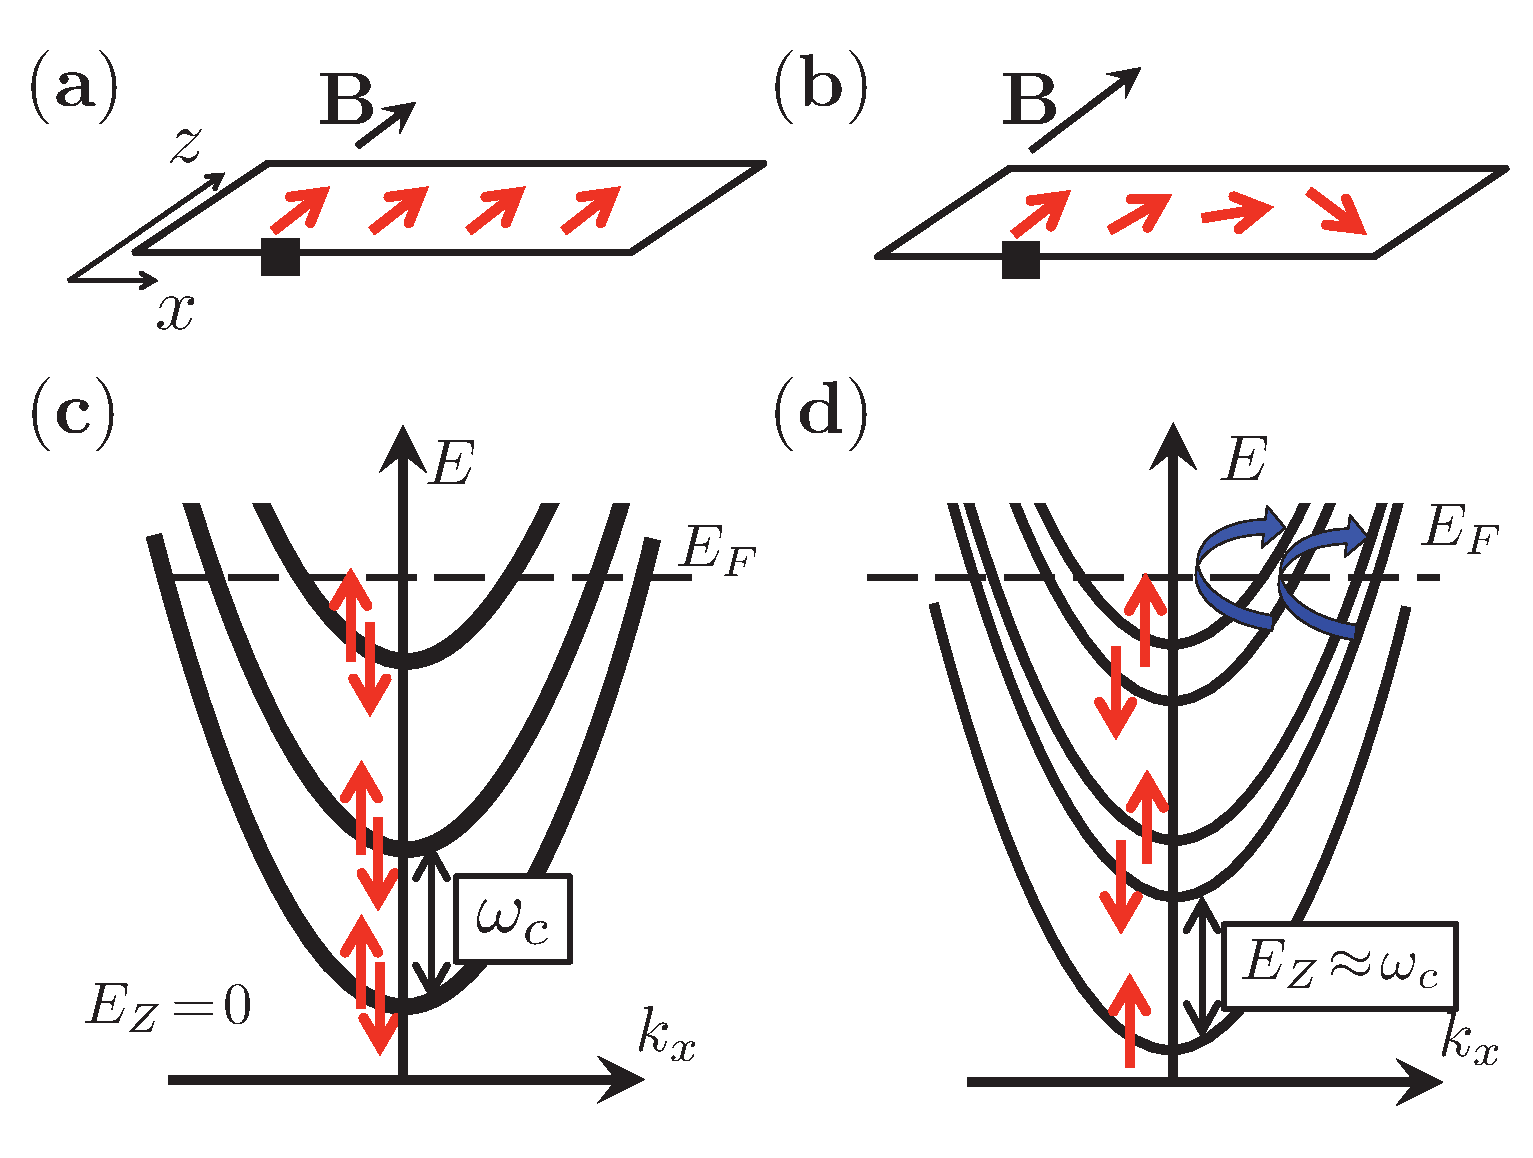
\includegraphics[width=1.0\columnwidth]{fig1.eps}
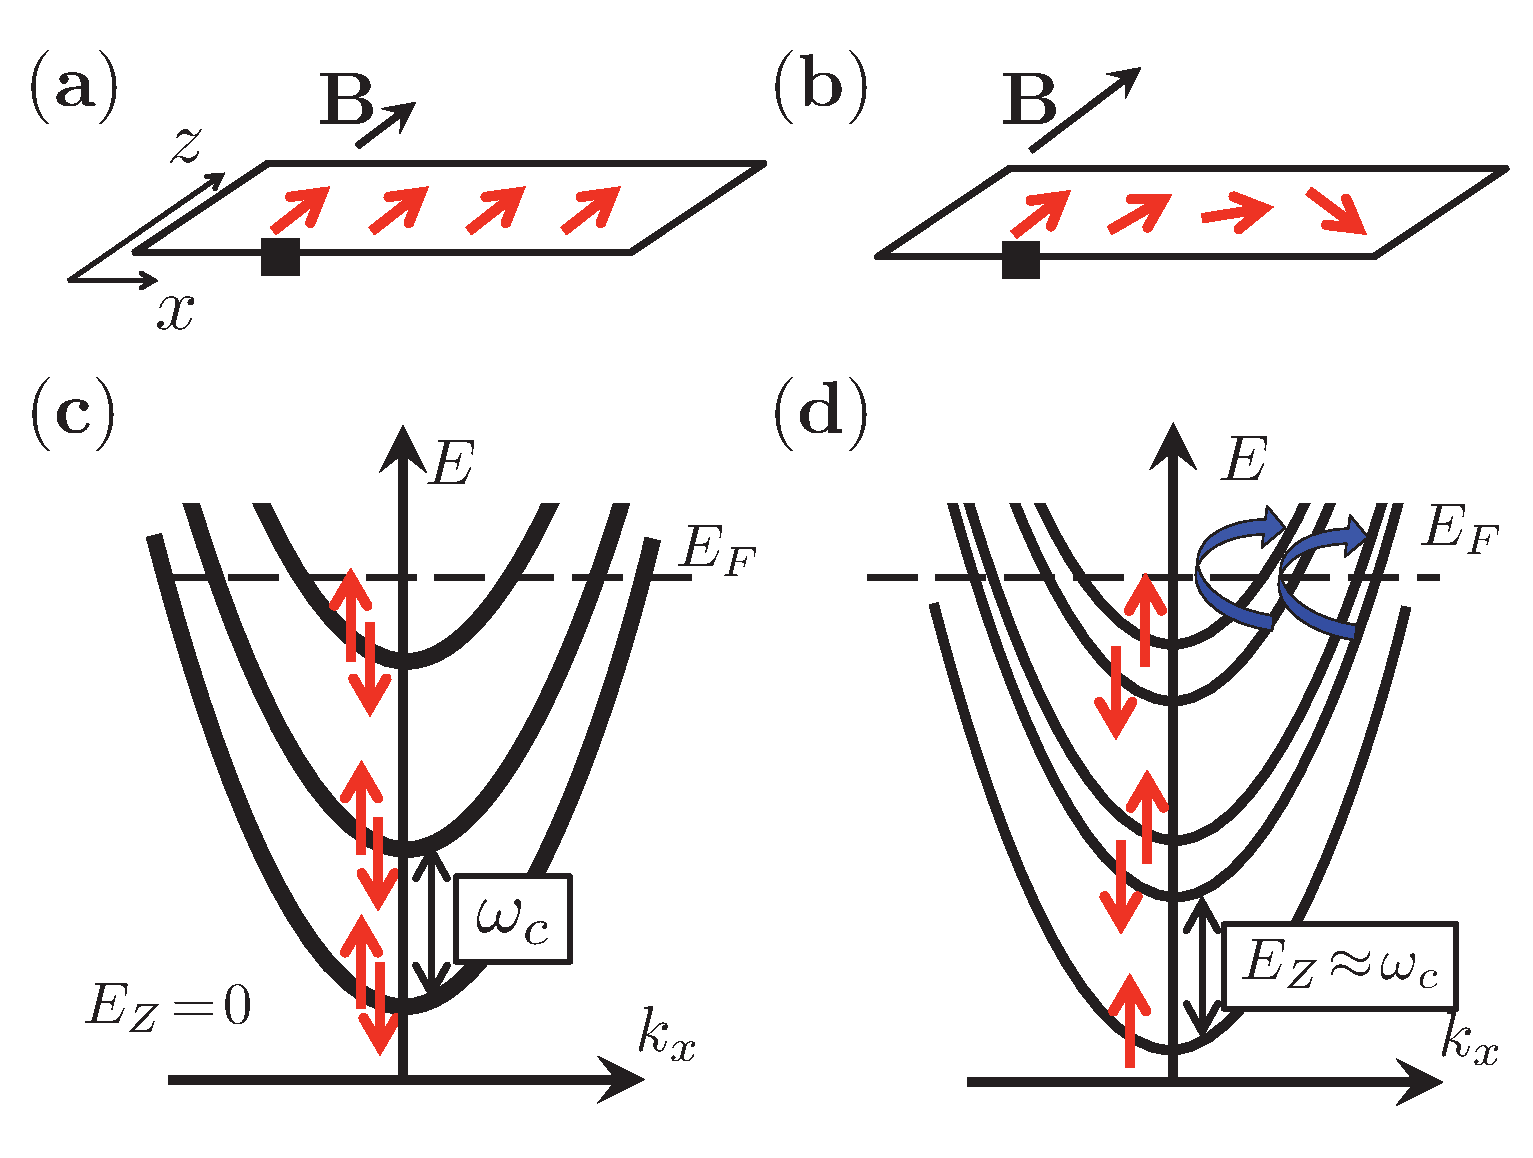
\includegraphics[width=0.5\columnwidth]{fig1.eps}
\caption{ (color online) 
(a) The spins shown as (red) straight arrows injected into the channel via the quantum point contact denoted by a (black) square are polarized along the applied magnetic field, $\vec{B} \parallel \hat{z}$. 
The channel is running parallel to $x$ axis. 
Normally, they maintain their polarization in the course of propagation along the channel.
(b) At the BSR $E_Z \approx \omega_{\perp}$ the spins are still injected with the initial polarization along $\vec{B}$.
Their state of polarization however is modified as they move along the channel.
(c) In the absence of magnetic field the energy levels form subbands due to the quantization along $\hat{z}$.
For the parabolic confinement the subband splitting, $\omega_{\perp}$ is equal to the angular frequency of oscillations across the channel.
(d) At the BSR, $E_Z \approx \omega_{\perp}$ the adjacent subbands with opposite spin polarization are nearly degenerate.
The spin flip intersubband p-h excitations shown by thick round (blue) arrows become soft at the BSR, and play a central role in our analysis.\cite{Iqbal}}
\label{fig:setup}
\end{center}
\end{figure}


In our first work we analyze the effect of the electron-electron interaction on the BSR.


\section{Summary of Results}
%We start with the brief summary of our {\it main results}.

We consider the Fermi gas confined by a parabolic potential characterized by a frequency $\omega_{\perp}$ of the transversal motion. 
The local electron-electron interaction 
\begin{align}\label{M19}
\hat{H}_{\mathrm{int}} = \frac{1}{2} \int d \vec{r} \left[ V_{\rho} \left[\hat{\rho}(\vec{r})\right]^2 + 
V_s \hat{\vec{\sigma}}(\vec{r}) \cdot  \hat{\vec{\sigma}}(\vec{r}) \right]\,
\end{align}
is parametrized by amplitudes $V_{\rho}$ and $V_s$ of the interaction in the charge, $\hat{\rho}(\vec{r})$ and spin, $\hat{\sigma}(\vec{r})$ channels respectively.
Our main finding is that whereas for non-interacting system the BSR occurs at $B=B_{\mathrm{BSR}}$ such that the Zeeman splitting $E_Z = \omega_{\perp}$, in the presence of interaction Eq.~\eqref{M19} this field is renormalized,
\begin{align}\label{BSR_ren}
B^*_{\mathrm{BSR}} \approx B_{\mathrm{BSR}} \left[ 1 - 3 (V_{\rho} - 3 V_s) \nu/4 \right]\, .
\end{align}
The result \eqref{BSR_ren} holds for weak interaction, $\{ V_{\rho}\nu,  V_{s}\nu \} \lesssim 1$, where $\nu = m/\pi$ is the density of states of a Fermi gas of electrons of a mass $m$.
%
The result \eqref{BSR_ren} is obtained by combination of the two approaches: perturbation theory and the Fermi liquid phenomenology with local quasi-particle interaction.
The latter is applicable provided the channel width is much larger than the 
typical Fermi wavelength.
This condition is equivalent to the number of occupied subbands being large.
In the experiment \cite{Frolov2009} the Fermi energy of the electron gas at was $E_F \approx 4$meV corresponding to the density of $\approx 1.1 \times 10^{11}$cm$^{-2}$ in the high mobility GaAs-based heterostructures.
The reported magnetic field at the onset of the BSR on the other hand was $\approx 7$T. 
This gives $\omega_{\perp} \approx 0.15$meV for the bulk $g$-factor of $-0.44$.
The number of occupied subbands was therefore $E_F/\omega_{\perp} \approx 27 \gg 1$, and the Fermi liquid description applies.
% 

In a Fermi gas when the Zeeman splitting is tuned into the resonance, $E_Z = \omega_{\perp}$ the spin flip intersubband  particle-hole (p-h) excitations shown by round arrows in Fig.~\ref{fig:setup}(d) become soft, i.e. with nearly zero excitation energy.
Perturbation theory shows that although the energy of each such pair is modified by interaction, different p-h remain degenerate. 
It follows that the BSR can be meaningfully defined for $\{ V_{\rho}\nu,  V_{s}\nu \} \lesssim 1$.
As interaction causes the detuning of the BSR the condition for the BSR is modified in turn.

The second ingredient leading to Eq.~\eqref{BSR_ren} is the relation of the BSR to the spin density oscillations across the channel, or to the collective spin sloshing mode (see Fig.~\ref{fig:slosh}).
The perturbation theory indicates that the energy of this mode is very close to the spin flip intersubband  p-h excitations.
This observation links the BSR to the collective behavior.
We studied the spin sloshing mode within the phenomenological Fermi and obtained for its frequency
\begin{align}\label{result1_b}
\omega_{s}(E_Z) \approx 
E_Z  - \omega_{\perp} +(V_{\rho} \! -\!  3 V_s)\nu
(\omega_{\perp}/2 + E_Z/4)
\end{align}
valid under the same conditions as Eq.~\eqref{BSR_ren}.
The latter readily follows from Eq.~\eqref{result1_b} since the BSR sets in for $E_Z = E_Z^*$ such that $\omega(E_Z^*)  = 0$.

As evidenced by the result \eqref{result1_b} the $B_{\mathrm{BSR}}$ is  renormalized because of the absence of what would be the equivalent of Kohn theorem \cite{Kohn1961} for spin sloshing mode.
At first glance the Kohn theorem for spin sloshing mode should hold.
Indeed, in the parabolic potential the frequency of the density oscillations across the channel, or of the so called sloshing mode is $\omega_{\perp}$ regardless of interaction.
This was first discussed theoretically  \cite{Dobson1994,Brey1989} and confirmed experimentally \cite{Wixforth1994} in the context of semiconductor quantum wells, and more recently in relation to trapped cold fermions in optical lattices, \cite{Minguzzi2001,Chiacchiera2009}. 
Similarly, the Zeeman splitting gives rise to a collective spin precession mode which is similarly not renormalized according to another version of the Kohn theorem \cite{Yafet1963}.
As neither $\omega_{\perp}$ nor $E_Z$ is renormalized it is tempting to conclude that the frequency of the spin sloshing mode assumes its
non-renormalized value, $\omega_s = | \omega_{\perp} - E_Z|$.
Correspondingly, the spin sloshing mode and the p-h excitations degenerate with it soften at $E_Z = \omega_{\perp}$.
As a result one would mistakenly conclude that interactions do not modify the condition for BSR. 

To see why the BSR {\it is} nevertheless shifted by the interaction in accordance with Eq.~\eqref{BSR_ren} it is necessary to identify the collective degree of freedom unaffected by interactions whenever the Kohn theorem applies. 
In the case of the sloshing mode such degree of freedom is the center of mass, $d_z =\sum_i z_i$.
Here $z_i$ is the location of the $i$th electron.
In the case of spin precession such observable is the total spin, $\vec{\sigma} = \sum_{i} \vec{\sigma}_i$. 
The collective variable associated with the spin sloshing mode is $\sum_{i} z_i \vec{\sigma}_i$ inducing the transitions shown in Fig.~\ref{fig:setup}(d).
In contrast to $d_z$ and $\vec{\sigma}$, the observable $\sum_{i} z_i \vec{\sigma}_i$ in general does not commute with the interaction Hamiltonian.
This is the underlying reason for the absence of the Kohn theorem for the spin sloshing mode.
The situation similar in this regard arises for the chiral spin resonance when the transitions between spin-orbit split bands are induced by an ac electric field \cite{Shekhter2005}.
In the remainder of the paper we expand upon the above results.


The paper is organized as follows.
In Sec.\ref{sec:Fermi} we develop the hydrodynamic approach based on Fermi liquid to describe the three collective excitations: sloshing mode, spin precession mode and spin sloshing mode analyzed in Secs.~\ref{sec:Sloshing_mode}, \ref{sec:Collective_spin} and \ref{sec:Collective_spin-sloshing} respectively.
In Sec.~\ref{sec:Microscopic} we analyze on the spin-sloshing mode using the perturbation theory.
We compare the results obtained in Secs.~\ref{sec:Collective_spin-sloshing} and \ref{sec:Microscopic} in Sec.~\ref{sec:Comparison}.
Following the comparison the effect of interaction on BSR is presented in Sec.~\ref{sec:Interaction}.
The results are summarized and discussed in Sec.~\ref{sec:Conclusions}. 
Some of the technicalities are relegated to appendices.

\section{Fermi Liquid Theory of Spin-Sloshing Mode}
\label{sec:Fermi}

In this section we study the three types of collective excitations in parabolically confined Fermi liquid: the sloshing mode, the spin precession and the spin sloshing mode.
Crucially, while the BSR requires finite spin-orbit interaction, the condition for its onset does not depend on it.
For that reason here we limit the consideration disregarding the spin-orbit interaction.
See Ref.~\cite{Chen1999,Ashrafi2012,Ashrafi2013} for the discussion of the Fermi liquid effects specific for systems with spin-orbit interaction.

\subsection{Sloshing Mode in Fermi Liquid Confined by a Parabolic Potential} 
\label{sec:Sloshing_mode}


Let the confining potential be $U(z) = k z^2/2$ and the equilibrium distribution function $n_0( \epsilon_{\vec{p}}(z) )$.
The Kohn mode is the solution of Eq.~\eqref{FL1} of the form \cite{Chiacchiera2009,Pantel2012},
\begin{align}\label{FL5a}
\delta n^K_{\vec{p}}(z) = 
[\partial_{ \epsilon_{\vec{p}}} n_0( \epsilon_{\vec{p}}(z) )]e^{- i \omega t}
\left( a_{\omega} z   + b_{\omega} \cos \theta_{\vec{p}} \right)
\end{align}
describing oscillations of the particle and current density across the channel at frequency $\omega$.
In Eq.~\eqref{FL5a} we denote by $\theta_{\vec{p}}$ the angle the quasi-particle momentum forms with $z$-axis directed perpendicular to the channel, see Fig.~\ref{fig:setup}(a).
It follows that $\cos \theta_{\vec{p}} = p_z/ p_F$, where $p_F(z)$ is the Fermi momentum.
The density oscillations represented by Eq.~\eqref{FL5a} have a vanishing amplitude at the center of the channel, $z=0$, and grow linearly away from it.
The equation \eqref{FL5a} therefore describes the collective sloshing of the Fermi liquid across the channel, and is referred to as the sloshing mode.

We show that in the Galilean invariant system the non-trivial solutions to Eq.~\eqref{FL1} of the form \eqref{FL5a} exists for the choice $\omega = \omega_{\perp}= \sqrt{k/m}$ determined by the bare electron mass and not sensitive to the interaction.
The statement of the existence of the sloshing mode with unrenormalized frequency $\omega_{\perp}$  is general and does not depend on the statistics or temperature. 
Below we demonstrate it for the Galilean invariant Fermi liquid, setting the stage for the discussion of the spin sloshing mode.

Thanks to the particle and momentum conservation, $I[\delta n^K]=0$ and substitution of Eq.~\eqref{FL3} into Eq.~\eqref{FL1} yields to the linear order in $\delta n^K$,
\begin{align}\label{FL6a}
- i \omega \delta n^K + \{\sum_{\vec{p'}} f_{\vec{p}\vec{p}'} \delta n^K_{\vec{p}'}, n^0 \} 
+
\{ \epsilon_{\vec{p}},  \delta n^K \} = 0\, .
\end{align}
%
In the second term of Eq.~\eqref{FL6a} we have 
\begin{align}\label{FL7a}
\sum_{\vec{p}'} f_{\vec{p}\vec{p}'} \delta n^K_{\vec{p}'} = 
-e^{ -i \omega t} \left[F_0 z a_{\omega} + F_1 b_{\omega} \cos \theta_{\vec{p}}\right]\, ,
\end{align}
%where the Landau parameters are defined by the Fourier expansion 
%$\nu^* f_{\vec{p}\vec{p}'} = \sum_{m=-\infty}^{\infty} F_m  e^{i m (\theta_{\vec{p}}-\theta_{\vec{p}'})}$.
%Here quasi-particle density of states $\nu^* = m^*/\pi$ is proportional to the effective mass $m^*$.
The momentum derivative of the equilibrium distribution function in Eq.~\eqref{FL6a} reads
\begin{align}\label{FL9a}
\partial_{p_z} n_0 =\left[ \partial_{\epsilon} n_0\right]\left( p_z/ m^*\right)
\end{align}
as by definition $1/m^* = \partial_{p_z} \epsilon_{\vec{p}}(z) / p$ evaluated at $p = p_F$.
For the spatial derivative we have, $\partial_z n_0= \left[\partial_{\epsilon} n_0\right] \partial_z \epsilon_{\vec{p}}(z)$, where
\begin{align}\label{FL11}
\partial_z \epsilon_{\vec{p}}(z)=  \frac{ \partial_z U(z) }{ 1 + F_0 }\, .
\end{align}
The equation \eqref{FL11} can be understood as follows.
Let the quasi-particle be translated from the Fermi surface at $z$ to the Fermi surface at $z+dz$ as shown in Fig.~\ref{fig:FL1} as path A.
At equilibrium the free energy should be the same before and after the translation,
\begin{align}\label{FL13}
 U(z\!+\! d z) - U(z) \!=\!v_F\! \left[ p_F(z) - p_F(z\!+\!dz) \right]\!(1 + F_0),
\end{align}
where $v_F = p_F/ m^*$ is the Fermi velocity.
The term $\propto F_0$ accounts for the interaction of the trial quasi-particle with the Fermi surface deformation it sees as a result of a spatial translation by $dz$ see Fig.~\ref{fig:FL1}.
Equation \eqref{FL13} gives 
\begin{align}\label{FL15}
v_F \frac{ d p_F(z) }{ d z } = - \frac{ \partial_z U}{ 1 + F_0}\, .
\end{align}
We now translate the quasi-particle from $z$ to $z+dz$ while keeping its momentum constant, as shown in Fig.~\ref{fig:FL1} as path B.
The energy change as a result of this translation is
\begin{align}\label{FL17a}
d \epsilon_{\vec{p}}(\vec{r}) = \left[U(z+dz) - U(z)\right] + v_F d p_F F_0\, , 
\end{align}
where the first term is the change in the confining potential, and the second term is due to the interaction with an extra quasi-particles with momenta in the annulus of the width $dp_F$, $p_F(z)< p < p_F(z+dz)$.
Combination of Eqs.~\eqref{FL15} and \eqref{FL17a} gives Eq.~\eqref{FL11}.


\begin{figure}[ht!]
\begin{center}
%\includegraphics[width=1.0\columnwidth]{fig2.eps}
\includegraphics[width=0.5\columnwidth]{fig2.eps}
\caption{ (color online) 
The two Fermi surfaces located at $z$ and $z+dz$ shown as solid circles.
As the confining potential $U(z)$ decreases with $z$ the Fermi momenta at the two points satisfy $p_F(z+dz) > p_F(z)$.
When a quasi-particle is transferred from $z$ to $z+dz$ its energy changes partly due to the interaction with the quasi-particles in the annulus $p_F(z) <  p < p_F(z+dz)$ (grey) of a radius $dp_F$. 
This interaction is an ultimate cause of the force renormalization, Eq.~\eqref{FL11}.
For the quasi-particle transferred along the path A the energy change is zero.
The translation along path B with momentum kept constant is used to derive Eq.~\eqref{FL11}.\cite{Iqbal}}
\label{fig:FL1}
\end{center}
\end{figure}


Substituting Eqs.~\eqref{FL7a}, \eqref{FL9a} and \eqref{FL11} in Eq.~\eqref{FL6a}, and equating both the linear in $z$ and linear in $p_z$ parts to zero we obtain,
\begin{align}\label{FL21}
i \omega a_{\omega} - b_{\omega} \frac{ k}{ p_F}\frac{ 1 + F_1 }{ 1 + F_0}  &= 0
\notag \\
a_{\omega} v_F ( 1 + F_0) + i \omega b_{\omega}   & = 0 \, .
\end{align}
The non-trivial solution of \eqref{FL21} is obtained for $\omega^2 = (k/m^*)(1 + F_1) $.
And in view of the Galilean invariance, \eqref{Galileo}
we recover the Kohn mode with frequency $\omega = \omega_{\perp}$.
%%%%%%%%%%%%%%%%%%%%%%%%%%%%%%%%%%
%
%
\subsection{Collective Spin Precession Mode in a Confined Fermi Liquid}
\label{sec:Collective_spin}
We now consider the collective spin precession mode in the presence of an in-plane magnetic field $\vec{B}$.
For definiteness we assume that $\vec{B} \parallel \hat{z}$. 
In the absence of interactions spin of $i$-th electron, $\vec{\sigma}_i$ precesses with the frequency $E_Z$ equal to the Zeeman splitting.
As the spin conserving interaction commutes with the total spin, 
the latter precesses at the same unrenormalized frequency $E_Z$ as in the non-interacting case.

We show that this statement holds when the Fermi liquid is spatially confined.
In order to describe the spin dynamics we consider the distribution function as a density matrix in spin space, and generalize the transport equation \eqref{FL1} to \cite{Pitaevskii1980}
\begin{align}\label{kin_eq}
\partial_t  \hat{n}_{\vec{p}}(\vec{r}) \!+\! i[\hat{\tilde{\epsilon}}_{\vec{p}}(\vec{r}),\! \hat{n}_{\vec{p}}(\vec{r})]\! +\!
\{\hat{\tilde{\epsilon}}_{\vec{p}}(\vec{r}), \!\hat{n}_{\vec{p}}(\vec{r})\}\!=\! I[\hat{n}_{\vec{p}}(\vec{r})],
\end{align}
where the commutator of the two matrices is $[A,B] = AB - BA$.
%For the bare Zeeman coupling term, $\hat{H}_Z = g_0 \mu_B B /2 \sigma_z$, the quasi-particle energy takes the form
The quasi-particle Hamiltonian 
\begin{align}\label{SP1}
\hat{\tilde{\epsilon}}_{\vec{p}}\! =\! 
\epsilon_{\vec{p}}\! +\! \sum_{\vec{p}'}\left[ g_{\vec{p}\vec{p}'} \vec{\sigma} \Tr (\vec{\sigma}' \hat{\delta n}_{\vec{p}'})
+ f_{\vec{p}\vec{p}'} \Tr ( \hat{\delta n}_{\vec{p}'})\right]
-\frac{E_Z^r}{2}\sigma_z\, ,
\end{align}
where Tr stands for the trace over spin indices.
The last term on the right hand side of Eq.~\eqref{SP1} is the renormalized Zeeman coupling, \cite{Pitaevskii1980} 
\begin{align}\label{Zeeman_bare}
E_Z^r = E_Z(1 +G_0)^{-1}\, . 
\end{align}
Here and below we neglect the dependence of the Fermi liquid parameters on the magnetic field.
Such an approximation is satisfied as long as $E_F \gg E_Z$.
In a particular setup of Ref.~\cite{Frolov2009} the above condition is safely satisfied.
The collective spin precession is described by the density matrix 
\begin{align}\label{SP2}
\hat{n}_{pr} = n_0  + [\partial_{\epsilon} n_0] \frac{E_Z^r}{2}\sigma_z + [\partial_{\epsilon} n_0] e^{-i \omega t} A \sigma_{\pm}\, ,
\end{align}
where $\sigma_{\pm} = \sigma_x \pm i \sigma_y$.
The second term of Eq.~\eqref{SP2} stands for the equilibrium polarization of the Fermi liquid.
Due to the spin conservation, $I[\hat{n}_{pr} ]  = 0$.
As the precession amplitude $A$ is position independent the Poisson bracket term of Eq.~\eqref{kin_eq} vanishes for the solution of the form \eqref{SP2}.
The quasi-particle energy Eq.~\eqref{SP1} takes the form
\begin{align}\label{SP3}
\hat{\tilde{\epsilon}}_{\vec{p}} = 
\epsilon_{\vec{p}} 
- \frac{E_Z^r}{2}\sigma_z
- G_0 A \sigma_{\pm} e^{-i \omega t} 
\end{align}
for the distribution function Eq.~\eqref{SP2}.\\
 Here we have introduced $\nu^* g_{\vec{p}\vec{p}'} = \sum_{m=-\infty}^{\infty} G_m e^{i m (\theta_{\vec{p}}-\theta_{\vec{p}'})}$.
We obtain for the commutator of Eq.~\eqref{SP2} and Eq.~\eqref{SP3}
\begin{align}\label{SP4}
[\hat{\tilde{\epsilon}}_{\vec{p}},\hat{n}_{pr}] = -A E_Z^r (1 + G_0) \sigma_{\pm} e^{-i \omega t}\, .
\end{align}
Substitution of Eqs.~\eqref{SP4} in Eq.~\eqref{kin_eq} shows that the equation \eqref{SP2} is a solution with unrenormalized frequency $\omega = E_Z^r (1 + G_0) = E_Z$ as expected.
%%%%%%%%%%%%%%%%%%%%%%%%
\subsection{Collective Spin-Sloshing Mode}
\label{sec:Collective_spin-sloshing}
In this section we construct and analyze the spin sloshing mode.
It combines features of both Kohn mode and collective spin precession mode discussed in Sec.~\ref{sec:Sloshing_mode} and \ref{sec:Collective_spin} respectively.
This mode is important because as we will show in Sec.~\ref{sec:Interaction} it provides us with the information on the interaction induced renormalization of the BSR.
In the spin sloshing mode the density does not change but the spin density undergoes precession with the amplitude vanishing at the center of the channel and growing linearly away from it, see Fig.~\ref{fig:slosh}.

\begin{figure}[ht!]
\begin{center}
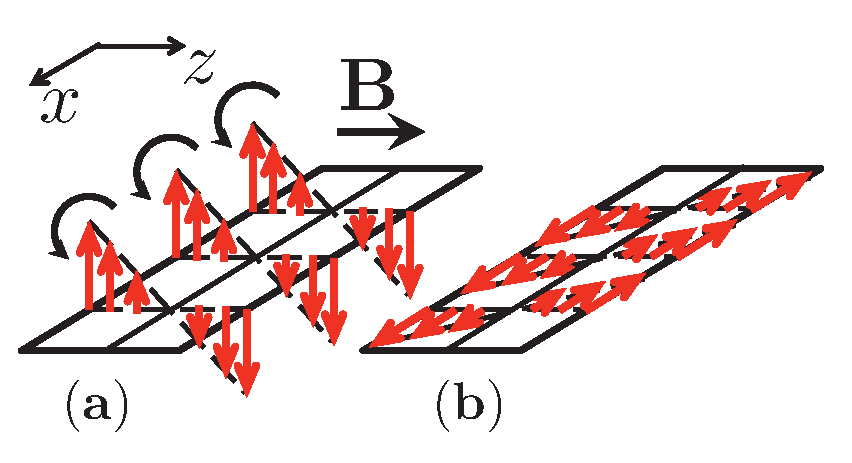
\includegraphics[width=0.5\columnwidth]{fig3.eps}
\caption{ (color online) The representation of the spin sloshing mode.
The magnetic field $\vec{B}$ is assumed to point in $z$-direction perpendicular to the channel running along $x$-direction. 
Thick arrows (red) represents the spin polarization changing across the channel, and vanishing at its center, $z=0$.
The profile is translationally invariant along the channel and all the spins collectively precesses at frequency $\omega_s$.
(a) The snapshot of spin polarization at an instant such that the polarization is perpendicular to the $xz$-plane.
(b) In a quarter period of precession, $\pi/2 \omega_{\perp}$ the spin polarization starting in a configuration shown in (a) rotates by $90^{\circ}$ and becomes parallel to the $xz$-plane.\cite{Iqbal}}
\label{fig:slosh}
\end{center}
\end{figure}






Accordingly, the trial solution of the transport equation \eqref{kin_eq} describing the spin sloshing mode is 
\begin{align}\label{ansatz}
\hat{n}_{s} =  n_0   + [\partial_{\epsilon} n_0] 
\left(
e^{- i \omega t}( a_{\omega} z + b_{\omega} \cos \theta_{\vec{p}}) \sigma_{\pm} - \frac{E_Z^r}{2}\sigma_z  \right)\, ,
\end{align}
where similar to Sec.~\ref{sec:Collective_spin} we assume $\vec{B} \parallel \hat{z}$.
We look for the frequencies $\omega$ such that Eq.~\eqref{ansatz} is the non-trivial solution of Eq.~\eqref{kin_eq} with $a_{\omega}^2 + b_{\omega}^2 \neq 0$. 
The quasi-particle Hamiltonian, \eqref{SP1} for the density matrix \eqref{ansatz} reads
\begin{align}\label{slosh1}
\hat{\tilde{\epsilon}}_{\vec{p}} = 
\epsilon_{\vec{p}} - \frac{E_Z^r}{2}\sigma_z
- e^{-i \omega t} ( a_{\omega} z G_0 + b_{\omega} G_1\cos \theta_{\vec{p}}) \sigma_{\pm}  \, .
\end{align}
We now substitute \eqref{ansatz} and \eqref{slosh1} in the transport equation, Eq.~\eqref{kin_eq} and find the frequency $\omega$ at which the expression \eqref{ansatz} is a non-trivial solution.


Unlike the particle and spin density the spin-current in general is not conserved and the collision term $I[\hat{n}_s]$ is in general non-zero.
Here we limit the consideration to the collisionless regime.
On general grounds collisions lead the attenuation of the spin sloshing collective mode.
For the low temperatures studied in the experiment \cite{Frolov2009} electron-electron collision induced broadening can be assumed to be negligible.
 
In contrast to Eq.~\eqref{SP3} obtained for the collective spin precession Eq. \eqref{slosh1} contains the coordinate $z$ explicitly.
It follows that both the commutator and the Poisson brackets terms of Eq.~\eqref{kin_eq} are non-zero for Eq.~\eqref{ansatz}.
The commutator term in \eqref{kin_eq} can be easily computed yielding 
\begin{equation}\label{slosh2}
 [ \hat{\tilde{\epsilon}}, \hat{n}] =  
\mp  E_Z^r e^{-i \omega t} \sigma_{\pm}  [\partial_{\epsilon} n_0 ]\left( a_{\omega} z G_0^+ + b_{\omega} \cos \theta_{\vec{p}} G_1^+ \right),
\end{equation}
where we have introduced the notation $G_n^+ = G_n+1$ and similarly,
$F_n^+ = F_n +1$ for shortness.

The linearized expression for the Poisson bracket term in Eq.~\eqref{kin_eq} can be obtained from the following expressions for the derivatives of the quasi-particle Hamiltonian, Eq.~\eqref{slosh1}
\begin{subequations}\label{slosh3}
\begin{align}\label{slosh3a}
\partial_z \hat{\tilde{\epsilon}} & = \partial_z \epsilon_{\vec{p}} - e^{-i \omega t } a_{\omega} G_0 \sigma_{\pm}
\end{align}
\begin{align}\label{slosh3b}
\partial_{p_z} \hat{\tilde{\epsilon}} & = \frac{p_z}{m^*} - e^{-i \omega t } b_{\omega}  \frac{G_1}{p_F} \sigma_{\pm}\, ,
\end{align}
\end{subequations}
and the derivatives of the density matrix, Eq.~\eqref{ansatz}
\begin{subequations}\label{slosh4}
\begin{align}\label{slosh4a}
\partial_z \hat{n}_s & = [\partial_{\epsilon} n_0]
\left( \partial_z \epsilon_{\vec{p}} + a_{\omega} e^{-i \omega t} \sigma_{\pm} \right)
\end{align}
\begin{align}\label{slosh4b}
\partial_{p_z} \hat{n}_s & = [\partial_{\epsilon} n_0]
\left( \frac{p_z}{m^*} + \frac{b_{\omega}}{p_F} e^{ - i \omega t} \sigma_{\pm} \right)\, .
\end{align}
\end{subequations}
In writing Eq.~\eqref{slosh3a} the spatial derivatives of the Fermi liquid parameters were neglected.
These derivatives are expected to be small for large number of occupied subbands.
The reason is the slow variation of the Fermi liquid parameters in this high density and shallow confinement regime.
Note that in the considered case of a confined two-dimensional systems with weak and short-range interaction this approximation becomes exact because of the independence of the density of states on the particle concentration in two dimensions.
This justification is elaborated in Sec.~\ref{sec:Comparison} where we compare the results of Fermi liquid analysis with the microscopic calculations.

Using the Eqs.~\eqref{slosh3} and \eqref{slosh4} we obtain for the linearized Poisson bracket entering Eq.~\eqref{kin_eq}
\begin{align}\label{slosh5}
\{\hat{\tilde{\epsilon}}, \hat{n}_s\}=
[\partial_{\epsilon} n_0] e^{- i \omega t} \sigma_{\pm}
\left(
a_{\omega}G_0^+\frac{p_z}{m^*} - \frac{b_{\omega}}{p_F}G_1^+ \partial_z \epsilon_{\vec{p}}
\right).
\end{align}
Substitution of Eqs.~\eqref{slosh2} and \eqref{slosh5} along with Eq.~\eqref{FL11} and the expression for the time derivative $ \partial_t \hat{n} =- i \omega e^{-i \omega t} ( a_{\omega} z+ b_{\omega} \cos \theta_{\vec{p}}) \sigma_{\pm}$ into Eq.~\eqref{kin_eq} yields in the collisionless regime two conditions
\begin{align}\label{slosh6}
i  v_F a_{\omega}  \left( \omega \pm E_Z^r G_0^+\right) 
+b_{\omega}  \frac{k}{m^*} \frac{G_1^+}{F_0^+} &= 0
\notag \\
i  v_F a_{\omega}  G_0^+   + b_{\omega}  \left( \omega \pm E_Z^r G_1^+ \right) 
&=0\, .
\end{align}
The non-trivial solution of Eqs.~\eqref{slosh6} is obtained for $\omega = \omega_s$ and $\omega = \omega_f$ where
\begin{align}\label{result1}
\omega_{s,f} = 
& \left\vert 
 E_Z\frac{G_1^+  + G_0^+}{2  G_0^+}
\right.
\notag \\
&\,\, \left. \mp \sqrt{ \left[E_Z \frac{ (G_1^+ - G_0^+) }{  2 G_0^+ }\right]^2+ \omega_{\perp}^2 \frac{G_0^ +G_1^ +}{F_0^ +F_1^ +} }\right\vert \, .
\end{align}
The result Eq.~\eqref{result1} is stated in terms of bare frequencies $E_Z$ and $\omega_{\perp}$ through the Galilean invariance condition Eq.~\eqref{Galileo} and the relation \eqref{Zeeman_bare}.


The slow and fast collective modes with eigenfrequencies $\omega_s$ and $\omega_f$ are distinguished by their non-interacting limit.
In a free gas the two frequencies become $\omega_{f,s} = \left\vert\omega_{\perp} \pm E_Z\right|$.
Therefore, for not too strong interactions, at the onset of BSR the slow mode with frequency $\omega_s$ softens down. 
It is for this reason we henceforth focus on this mode.

We define $E_Z^*$ as the Zeeman splitting at which $\omega_s = 0$.
In the non-interacting Fermi gas we have $E_Z^* = \omega_{\perp}$.
In the Fermi liquid Eq.~\eqref{result1} gives
\begin{align}\label{result2}
E_Z^* = \omega_{\perp} \frac{ G_0^+ }{ \sqrt{ F_0^{+} F_1^{+}}}\, .
\end{align}
Both Eqs.~\eqref{result1} and \eqref{result2} refer to the collective excitations of a confined Fermi liquid.
The BSR on the other hand occurs when the individual quasi-particles satisfy the resonant condition.
Nevertheless, we demonstrate that the result \eqref{result2} bears on the renormalization of the BSR in the limit of weak interactions.
To this end in the next section we supplement the Fermi liquid phenomenology with the microscopic analysis.


\section{Microscopic Analysis: Perturbation Theory} 
\label{sec:Microscopic}
Our goal is to compute the frequency of the collective mode, $\omega_s$  in perturbation theory in interaction.
The microscopic calculation will provide us with the independent way to confirm the results Eq.~\eqref{result1} and \eqref{result2} obtained phenomenologically.
More importantly, it will allow us to relate the interaction induced shift of the BSR to the renormalization of the collective mode as given by Eq.~\eqref{result1}.
Here we focus on the spin sloshing mode.
The analogous analysis of the sloshing and spin precession modes is detailed in App.~\ref{app:Kohn}.


The Hamiltonian 
\begin{align}\label{M11}
\hat{H} = \hat{H}_0 + \hat{H}_{\mathrm{int}}\, ,
\end{align}
where the second term given by Eq.~\eqref{M19} describes the interaction, and the first is a free quadratic part,
\begin{align}\label{M13}
\hat{H}_0 = \sum_{n,\alpha,k_x} \psi_{n,\alpha;k_x}^{\dag} E_{n\alpha}(k_x)  \psi_{n,\alpha;k_x}\, ,
\end{align}
where  $\psi^{\dag}_{n,\alpha;k}$ is the operator creating an electron in the state $|n,k_x\rangle | \alpha \rangle$ such that
\begin{align}\label{M14}
\langle z,x |n,k_x \rangle  = \varphi_n(z/\ell) e^{i k_x x}  \, .
\end{align}
The first factor of the wave function \eqref{M14} is the standard harmonic oscillator wave functions  
\begin{align}\label{M14a}
\varphi_n(\xi) = (2^m m!)^{-1/2} \pi^{-1/4} \exp( - \xi^2/2  ) H_n( \xi )\, ,
\end{align}
where $H_n(\xi)$ is the Hermite polynomials, and the subband index $n$ is non-negative integer.
The oscillator length is $\ell = 1/ \sqrt{ m \omega_{\perp}}$.
The exponential prefactor describes the propagation of the electron with the momentum $k_x$ along the channel.
The spinors $|\alpha\rangle$ satisfy $\sigma_z |\alpha\rangle = \alpha |\alpha\rangle$ and for $\alpha = \pm 1$ describe the state of polarization along the in-plane magnetic field $\vec{B} \parallel \hat{z}$.
The dispersion relation of non-interacting electrons is 
\begin{align}\label{M17}
E_{n\alpha}(k_x) = \frac{k_x^2}{2 m } + \omega_{\perp} \left( n +\frac{1}{2}\right) - E_Z\frac{\alpha}{2} \, .
\end{align}
For fixed $n$ and $\alpha$ the states for all possible $k_x$ form subbands labeled here by $|n,\alpha\rangle$ for shortness.
For a given Fermi energy, $E_F$ if $E_{n\alpha}(k_x=0)  < E_F$ the subband $|n,\alpha \rangle$ crosses the Fermi level at the Fermi momentum
\begin{align}\label{kF}
k^F_{n,\alpha} = \sqrt{2 m \left[E_F - \omega_{\perp} \left( n +\frac{1}{2}\right) + E_Z\frac{\alpha}{2} \right] }\, .
\end{align}
It will be convenient to set $k^F_{n,\alpha} = 0$ for bands not crossing the Fermi level. 


\begin{figure}[h]
\begin{center}
\includegraphics[width=0.4\columnwidth]{fig5.eps}
\caption{(a) The scattering processes that leads to the most singular contributions to the correlation functions has both the initial and final states at resonance with the external frequency.
To the leading order this amplitudes contains the direct and exchange terms.
(b) The Dyson equation for the dressed Green function, Eq.~\eqref{Green} shown by the thick arrowed line combining the most singular contributions at the mass shell.
The thin line stands for the Green function of free electrons. 
(c) The Dyson equation for the matrix correlation function $\hat{\Gamma}$, Eq.~\eqref{Gamma} shown by the shaded area.
For the free electron gas $\hat{\Gamma}$ is given by the polarization operator, Eq.~\eqref{Polarization}.\cite{Iqbal}}
\label{fig:scattering}
\end{center}
\end{figure}




Our strategy is to sum exactly all the terms of perturbation theory in the interaction Eq.~\eqref{M19} of the form $\propto \left[ V_{\rho} (\omega - \delta \omega)^{-1} \right]^{n_1} \left[ V_{s} (\omega - \delta \omega)^{-1}\right]^{n_2} (\omega - \delta \omega)^{-1}$ with $n_{1,2}$ being a non-negative integer and we introduced the detuning 
\begin{align}\label{detuning}
\delta \omega = | E_Z - \omega_{\perp} |\, .
\end{align}
Such a procedure amounts to the summation of the most singular contributions for $\omega \approx \delta \omega$ at each order of perturbation theory.
It is accurate provided the interaction is sufficiently weak.
More precisely, the typical frequency shift due to the interaction should be smaller than the intersubband separation, 
$V_{\rho,s} \ell^{-2} \lesssim \omega_{\perp}$.
Introducing the unrenormalized density of states $\nu = m / \pi$ we arrive at the condition $\left\{ V_{\rho} \nu, V_s \nu \right\} \lesssim 1$.


To select the graphs giving the most singular contributions for $\omega \approx \delta \omega$ note that electron transitions between $|n+1,k_x\rangle |\alpha=+1 \rangle$ and $|n,k_x\rangle |\alpha=-1 \rangle$ states indicated by round arrows in Fig.~\ref{fig:setup}(d) are nearly at resonance with the frequency $\omega$. 
The amplitude of the scattering between the resulting p-h pairs brings for each factor of the interaction strength the singular combination $(\omega - \delta \omega)^{-1}$.
The above scattering processes are exemplified in Fig.~\ref{fig:scattering}(a).
The other class of equally singular contributions is the self-energy corrections (see Fig.~\ref{fig:scattering}(b)).
Indeed, the singularity in the propagator of a nearly degenerate pair is obtained when both particle and hole in the p-h pair are at the mass shell.
The self-energy insertions account for the on-shell singularities of particle and hole propagators separately, and should be therefore included on equal footing with the inter-pair scattering.


\begin{figure}[ht]
\begin{center}
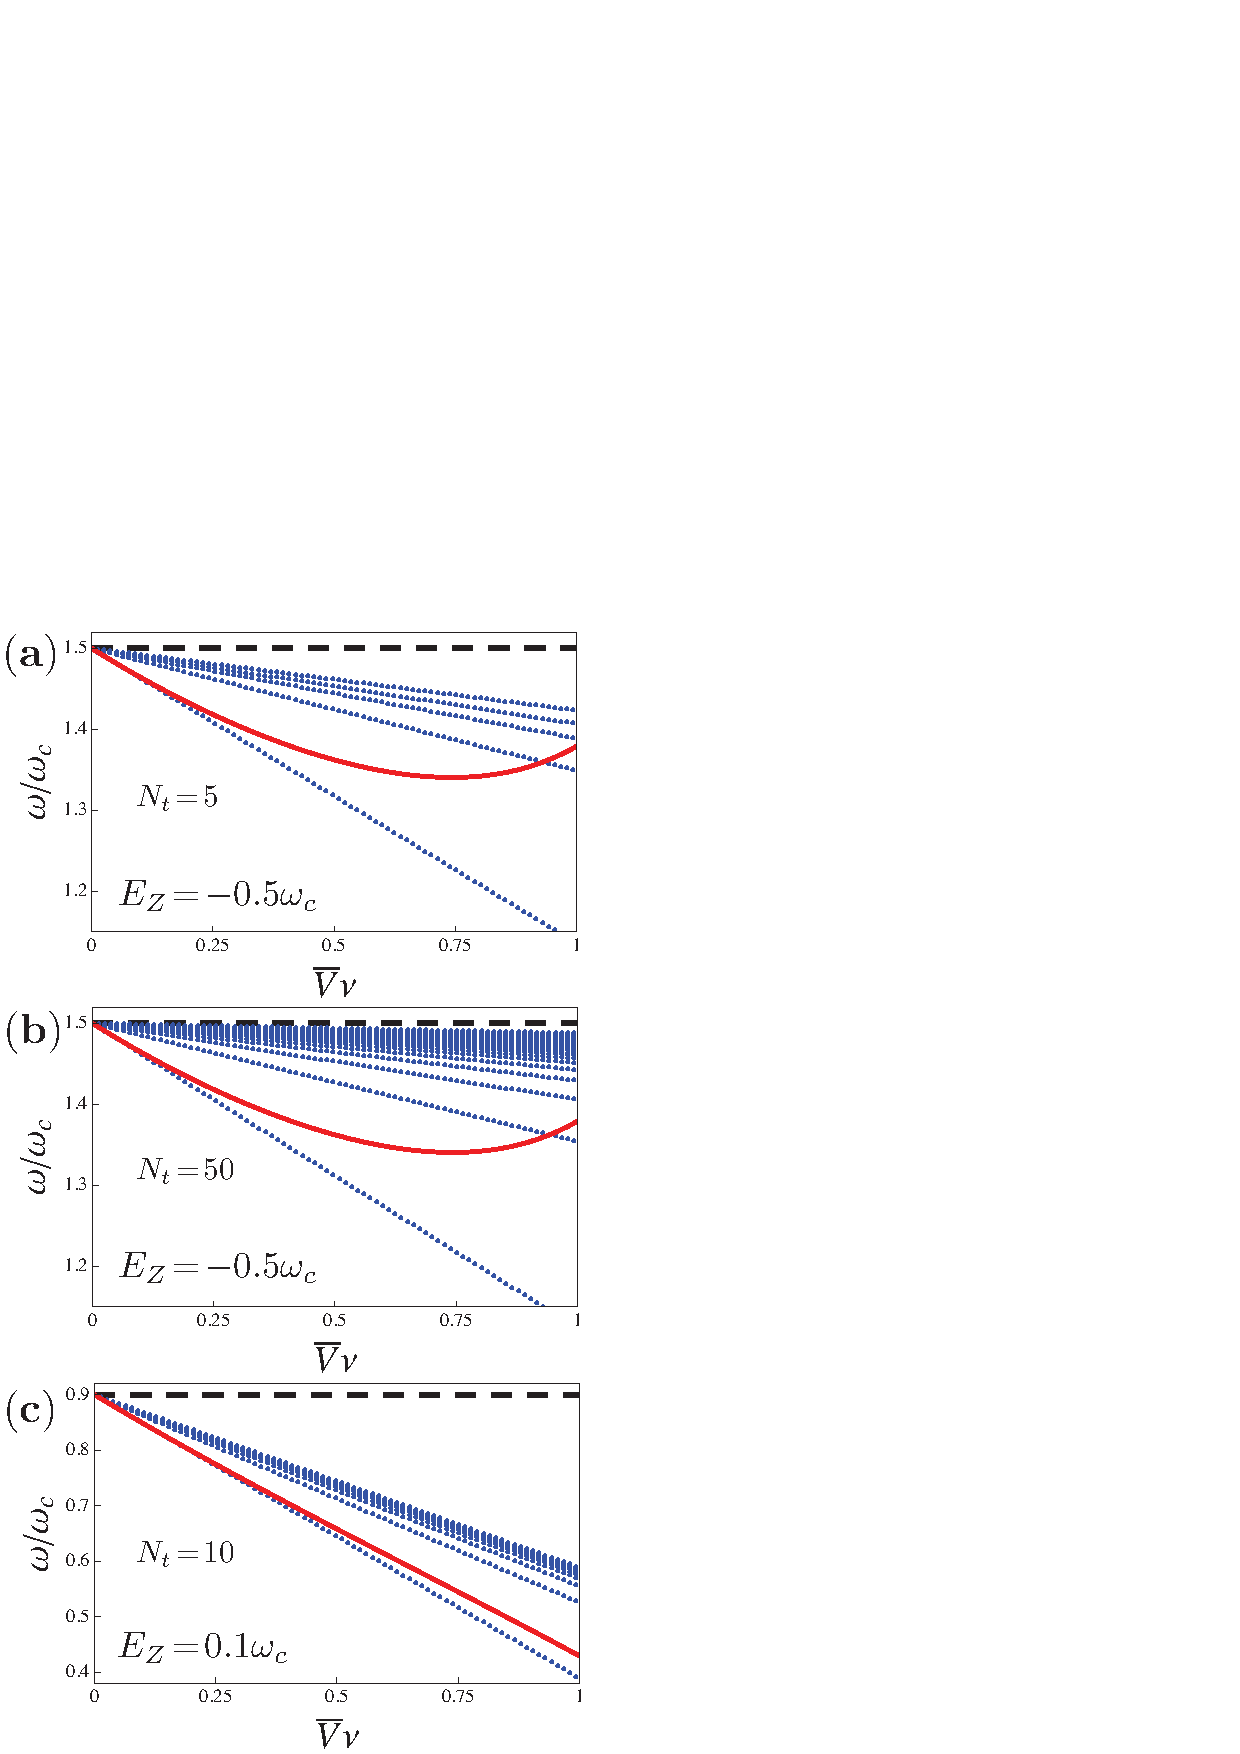
\includegraphics[width=0.9\columnwidth]{fig4.pdf}
\caption{ (color online) The dotted (blue) lines show the spectrum of collective modes that are superpositions of p-h excitations between the subbands $|n+1,+1\rangle$ and $|n,-1\rangle$ as a function of the interaction parameter $\bar{V} \nu =(V_{\rho} - 3 V_s) \nu$.
The solid (red) line is the frequency of the spin-sloshing mode as given by Eq.~\eqref{result1_a} obtained for the weakly interacting Fermi liquid. 
The horizontal dashed lines indicate the non-interacting excitation energy in units of $\omega_{\perp}$, $|\omega_{\perp} - E_Z|/\omega_{\perp}$.
The parameters used are (arb. units) $E_F = 50$,  $m=1$ and (a) $E_Z = -0.5 \omega_{\perp}$, $\omega_{\perp} = 10$, giving $N_t = 5$ according to Eq.~\eqref{Nt}; (b) $E_Z = -0.5 \omega_{\perp}$, $\omega_{\perp} = 1$, resulting in $N_t=50$ modes;
(c) $E_Z = 0.1 \omega_{\perp}$, $\omega_{\perp} = 5$, giving $N_t = 10$ modes.
The spin sloshing mode corresponds to the lowest energy mode of collective excitations.\cite{Iqbal}}
\label{fig:res1}
\end{center}
\end{figure}




To include most singular vertex and self energy corrections it is convenient to introduce the set of operators
\begin{align}\label{P}
P^{\dag}_{n} = \sum_{k} \psi_{n+1,+1, k}^{\dag} \psi_{n,-1, k}
\end{align}
creating the near degenerate p-h excitations.
The frequency of the collective spin-sloshing mode is given by the poles of the matrix correlation function
\begin{align}\label{Gamma}
\hat{\Gamma}_{nn'}(\omega) = \int_{-\infty}^{\infty} d t e^{  i \omega t}\left\langle T_t P_n(0) P^{\dag}_{n'}(t) \right\rangle\, ,
\end{align}
in a complex $\omega$ plane, and $T_{t}$ stands for the time ordering operation.
The indices $n$ and $n'$ running respectively over the $N_t$ rows and $N_t$ columns of the matrix $\hat{\Gamma}$ in Eq.~\eqref{Gamma} label the pairs of bands of the form $\{|n,-1\rangle, |n+1,+1 \rangle \}$ that can host p-h excitations created by the operators Eq.~\eqref{P}.
It follows that the dimensionality of $\hat{\Gamma}$, $N_t$ is equal to the number of such pairs with at least one subband crossing the Fermi level.
We have,
\begin{align}\label{Nt}
N_t = \mathrm{Int} 
\left[ \frac{E_F}{\omega_{\perp}} + \frac{1}{2} \left\vert \frac{|E_Z|}{\omega_{\perp}} - 1\right\vert \right]\, ,
\end{align}
where $\mathrm{Int} \left[ x \right]$ stands for the integer part of $x$.


The  summation of the most singular contributions amounts to solving the Dyson equation presented graphically in Fig.~\ref{fig:scattering}(c).  
This procedure amounts to the random phase approximation used to study the dispersion relation of collective modes in quasi-one-dimensional wires \cite{Li1989,Haupt1991}. 
The intersubband spin plasmons in quantum wells were studied within a density-functional formalism \cite{Ullrich2002,Ullrich2003}.


The Dyson equation is solved  in the matrix form,
\begin{align}\label{Gamma_D}
\hat{\Gamma}(\omega) = \left[ \hat{\Pi}^{-1}(\omega) + \hat{W} \right]^{-1}\, .
\end{align}
The frequencies of the collective excitations $\omega_{\mathrm{coll}}$ satisfy 
\begin{align}\label{det}
\det \left[ \hat{\Pi}^{-1}(\omega_{\mathrm{coll}}) + \hat{W} \right] = 0\, .
\end{align}
In the expression \eqref{Gamma_D} the polarization operator $\hat{\Pi}(\omega)$ is a diagonal matrix,\\
$\left[\hat{\Pi}\right]_{nn'}(\omega) = \delta_{nn'} \Pi_{n}(\omega)$,
\begin{align}\label{Polarization}
\Pi_{n}(\omega) = 
\int \frac{d k d \epsilon}{ (2 \pi)^2 }
G_{n+1,+1}(\epsilon+\omega,k)
G_{n,-1}(\epsilon,k)\, ,
\end{align}
where Green functions,
\begin{align}\label{Green}
G_{n\alpha}(\epsilon,k) = \left[ \epsilon - (E_{n\alpha}(k)-E_F)   - \Sigma_{n,\alpha}\right]^{-1}  
\end{align}
contains the self energy $\Sigma_{n,\alpha}$ calculated to the first order in interaction, 
\begin{align}\label{self1}
\Sigma_{m,\alpha} & =
\bar{V} \ell^{-1} \sum_{m'=0}^{N_t} \frac{k^F_{m',-\alpha}}{ \pi } M^{m,m'}_{m,m'} \, ,
\end{align}
where the charge and spin interaction amplitudes combine into a single combination 
\begin{align}\label{bar_V}
\bar{V} = V_{\rho}- 3 V_s \, ,
\end{align}
 and 
\begin{align}\label{M}
M^{n,n'}_{l,l'} = \int_{-\infty}^{\infty} d \xi \varphi_n(\xi) \varphi_{n'}(\xi) \varphi_l(\xi) \varphi_{l'}(\xi)\, . 
\end{align}
Note that the spin up(down) self energy in Eq.~\eqref{self1} is expressed via the Fermi momenta of the spin down(up) fermions as required by Pauli principle for the point-like interaction.
Consistent with the approximations made, the higher order corrections to the self energy as well as Green functions off-diagonal in the subband index are omitted.
The vertex $\hat{W}$ matrix in Eq.~\eqref{Gamma_D} is expressed through the integrals of the type \eqref{M} as 
\begin{align}\label{W}
W_{n,n'} =\bar{V} \ell^{-1} M^{n+1,n'+1}_{n,n'},
\end{align}



The substitution of Eq.~\eqref{Green} in Eq.~\eqref{Polarization} followed by the straightforward energy and momenta integrations yields
\begin{align}\label{Polarization1}
\Pi_{n}(\omega) = 
\frac{\pi^{-1} \left( k^F_{n,-1} - k^F_{n+1,+1}\right) }{
\omega -\omega_{\perp} + E_Z
-
\Sigma_{n+1,+1} + \Sigma_{n,-1}
}\, .
\end{align}
The Fermi momenta in the numerator of Eq.~\eqref{Polarization1} are given by Eq.~\eqref{kF} for free fermions as required by the consistency with our approximations.


The explicit expression \eqref{Polarization1} allows us to reformulate the  Eq.~\eqref{det} as an eigenvalue problem amenable to numerical analysis.
Using Eq.~\eqref{Polarization1} we write
\begin{align}\label{Polarization2}
\hat{\Pi} = \hat{K}^{-1} \left( \omega - \omega_{\perp} + E_Z + \hat{\Sigma} \right)\, ,
\end{align}
where we have introduced the two diagonal matrices,
\begin{align}\label{hat_K}
\left[\hat{K}\right]_{m,m'} = \frac{1}{\pi} \left( k^{F}_{m-1,-1} - k^{F}_{m,+1} \right)\delta_{m,m'}
\end{align}
%
and
\begin{align}\label{hat_Sigma}
\left[\hat{\Sigma}\right]_{m,m'} = \left(- \Sigma_{m,+1} + \Sigma_{m-1,-1}\right) \delta_{m,m'} \, .
\end{align}


The equation \eqref{Polarization2} allows us to rewrite the condition Eq.~\eqref{det} as
\begin{align}\label{det1}
\det \left[  \omega_{\mathrm{coll}} - \omega_{\perp} + E_Z + \hat{\Sigma}  + \hat{W} \hat{K}  \right] = 0\, .
\end{align}
The condition \eqref{det1} implies that if $\lambda_j$ are the eigenvalues of the matrix $\hat{\Sigma}  +\hat{W} \hat{K}$ the frequencies of the collective modes are given by 
\begin{align}\label{collect}
\omega_{\mathrm{coll}} = \left| \omega_{\perp} - E_Z - \lambda_j \right|\, .
\end{align}
The expression \eqref{collect} reduces the solution of Eq.~\eqref{det} to the eigenvalue problem.



Since both the self energy $\hat{\Sigma}$ and the vertex function $\hat{W}$ are proportional to $\bar{V}$ it is clear that the frequencies of eigenmodes, Eq.~\eqref{collect} are linear functions of $\bar{V}$.
This linearity is an artifact of the weak coupling approximation, $\bar{V} \nu \lesssim 1$.
The results for the solution of the Eq.~\eqref{det1} are shown as a function of the interaction strength in Fig.~\ref{fig:res1}(a,b)  for $E_Z = -0.5 \omega_{\perp}$ and in Fig.~\ref{fig:res1}(c) for $E_Z = 0.1 \omega_{\perp}$.
%
%
%
\subsection{Comparison of the Results Obtained in Fermi Liquid and by Perturbation Theory}
\label{sec:Comparison}
Here we compare the results obtained in Secs.~\ref{sec:Collective_spin-sloshing} and \ref{sec:Microscopic}.
We limit the discussion to the weak interaction, $V_{\rho}\nu, V_s \nu \lesssim 1$ when both approaches are applicable.

To be able to use the results Eqs.~\eqref{result1} and \eqref{result2} we have to find the expressions for the Fermi liquid parameters for the microscopic Hamiltonian specified by Eqs.~\eqref{M11} and \eqref{M19}. 
To the leading order in $V_{\rho,s}$ the only non-zero Fermi liquid parameters read 
\begin{align}\label{comp13}
F_0 = - G_0 = \frac{1}{2} \bar{V} \nu\, ,
\end{align}
where the combination $\bar{V}$ is defined by Eq.~\eqref{bar_V}.
See App.~\ref{app:Fermi} for the derivation of equation \eqref{comp13}.
To the leading order in interaction the Fermi liquid parameters in Eq.~\eqref{comp13} are position independent.
In general this is not the case, and a different procedure combing the phenomenology with the measurements is required as proposed in the context of trapped Fermi gases \cite{Chien2010}.

With the approximation \eqref{comp13} the result \eqref{result1} takes the form
\begin{align}\label{result1_a}
\omega_s \approx 
E_Z\frac{4 - \bar{V}\nu}{4 - 2\bar{V} \nu}  - \sqrt{ E_Z^2 \frac{ \bar{V}^2 \nu^2}{4( 2 - \bar{V}\nu)^2} + \omega_{\perp}^2 \frac{ 2 -\bar{V}\nu}{2 + \bar{V}\nu} }\, .
\end{align}
The expression \eqref{result1_a} is shown in Fig.~\ref{fig:res1} along with the numerical solutions for poles of Eq.~\eqref{Gamma}.
The agreement between the Fermi-liquid result \eqref{result1} and the perturbation theory is naturally achieved in the regime of weak interactions, $\bar{V}\nu \lesssim 1$.
The comparison between Fig.~\ref{fig:res1}(a) and Fig.~\ref{fig:res1}(b) indicates that the two approaches are found to agree already for $5$ occupied pairs of subbands. 

As the expression Eq.~\eqref{result1_a} is valid for $\bar{V} \nu \lesssim 1$ we expand it, and obtain the result \eqref{result1_b}.
Equations  \eqref{result1_b} and \eqref{result1_a} demonstrates the absence of Kohn theorem for the spin sloshing mode explicitly.
The frequency $\omega_s$ of the spin-sloshing mode shifts due to the interactions by a finite amount $\bar{V} \nu ( E_Z/4 + \omega_{\perp}/2 )$.


\subsection{Interaction-Induced Shift of the BSR}
\label{sec:Interaction}

The spin sloshing mode becomes soft for the special Zeeman splitting $E_Z^*$ such that $\omega_s(E_Z^*) =0$.
Solving Eq.~\eqref{result1_b} for $E_Z^*$ to the leading order in interaction we obtain 
\begin{align}\label{EZ_star}
E_Z^* \approx \omega_{\perp}( 1 - 3 \bar{V} \nu/4 )\, .
\end{align}
Equivalently, this expression follows from the expansion of the result \eqref{result2} in $\bar{V} \nu$ using Eq.~\eqref{comp13}.
The expression \eqref{EZ_star} is the value of the Zeeman splitting at which the spin sloshing mode has a zero energy.
It has been obtained within the Fermi liquid with parameters evaluated for the weak and short range interaction, Eq.~\eqref{M19}.

To relate Eq.~\eqref{EZ_star} to the interaction induced renormalization of the BSR we compare the spin-sloshing mode frequency given by Eq.~\eqref{result1_a} or Eq.~\eqref{result1_b} to the spectrum of the rest of the p-h excitations in the regime $\omega_{\perp} \approx E_Z$.
The results are presented in Fig.~\ref{fig:res_comp}.
 
\begin{figure}[h]
\begin{center}
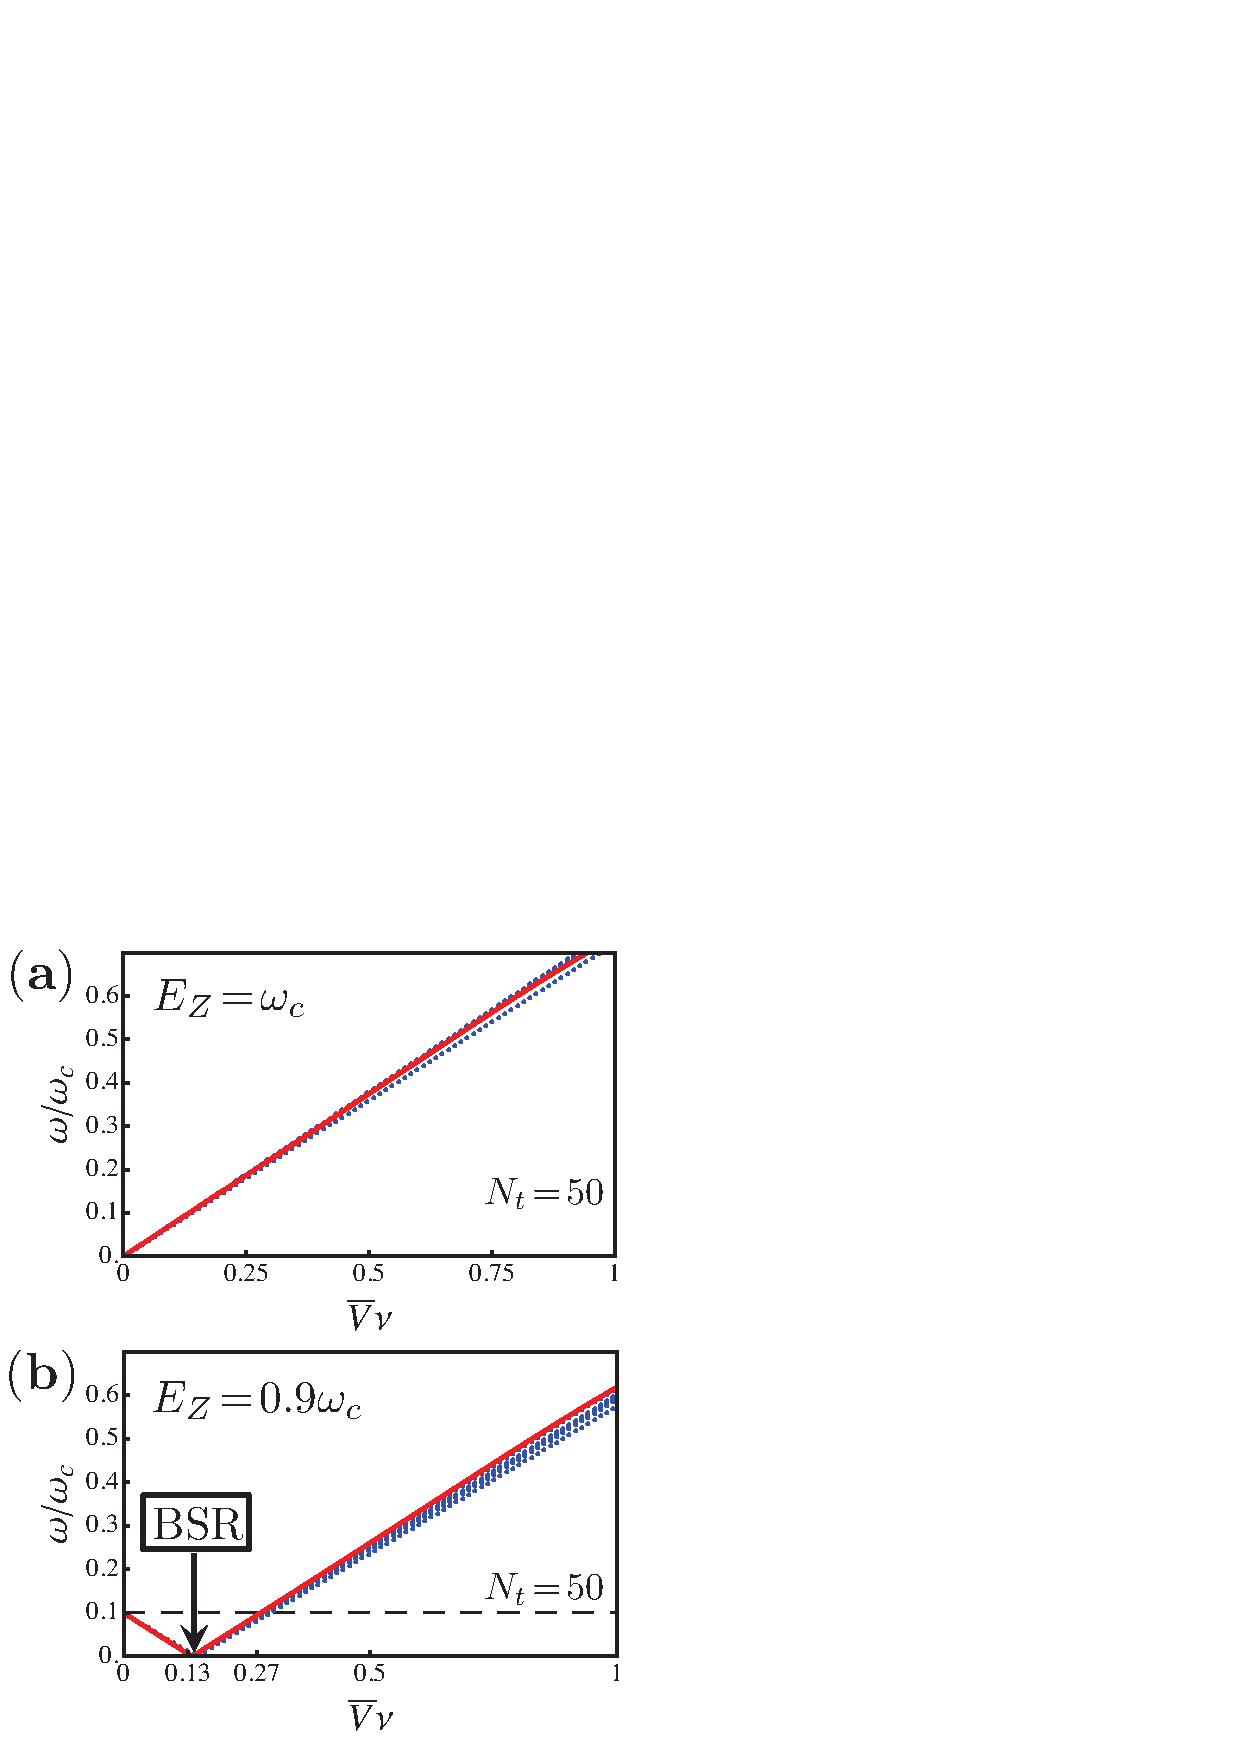
\includegraphics[width=0.7\columnwidth]{fig6.jpg}
\caption{ (color online) The dotted (blue) lines show the spectrum of p-h excitations between the subbands $|n+1,+1\rangle$ and $|n,-1\rangle$ as a function of the interaction parameter $\bar{V} \nu =(V_{\rho} - 3 V_s) \nu$.
The solid (red) line is the frequency of the spin-sloshing mode as given by Eq.~\eqref{result1_a}.
(a) At $E_Z = \omega_{\perp}$ the system is at resonance and goes off resonance at finite interaction.
(b) At $E_Z = 0.9\omega_{\perp}$ the resonance is achieved for 
$\bar{V} \nu = 40/3 \approx 1.33$ as follows from Eq.~\eqref{BSR_ren}.
The horizontal dashed lines indicate the non-interacting excitation energy  $|\omega_{\perp} - E_Z|/\omega_{\perp}$.
The parameters used are (arb. units) $E_F = 50$,  $m=1$, $\omega_{\perp} = 1$ corresponding to $N_t = 50$. 
The spin sloshing mode follows the continuum.\cite{Iqbal}}
\label{fig:res_comp}
\end{center}
\end{figure}

Figure \ref{fig:res_comp} shows how the p-h excitations involving the pairs of subbands of the form $|n+1,+1\rangle$ and $|n,-1\rangle$ change there energy with interaction for $E_Z = \omega_{\perp}$.
At no interaction all such pairs are zero energy excitations which is the condition for the onset of the BSR.
It follows that even for the number of p-h excitations as large as $N_t=50$ the interaction causes the same energy shift for all the p-h excitations.
In other words, the p-h pairs stay degenerate even in the presence of interaction.
The spin sloshing mode has the same energy as the individual p-h pairs.
The reason for this is the vanishing of the polarization operator, Eq.~\eqref{Polarization1} for $k^F_{n,-1} - k^F_{n+1,+1}$.
As is evident from Fig.~\ref{fig:res_comp} that all the solutions follow the spin sloshing mode given by the Fermi-liquid expression \eqref{result1_a}. 
The spin sloshing mode is strongly coupled to p-h continuum and is a short-lived excitation.

Importantly the expression \eqref{result1_a} obtained within the Fermi liquid for its energy is at the same time the energy of the p-h excitations between the subband $|n+1,+1\rangle$ and subband $|n,-1\rangle$.
It follows that the condition for the BSR is the vanishing of $\omega_{\perp}$ 
which occurs at $E_Z = E_Z^*$ with $E_Z^*$ given by Eq.~\eqref{EZ_star}.
Then, the BSR renormalization due to interaction takes the form of Eq.~\eqref{BSR_ren}.
The result \eqref{BSR_ren} is illustrated in Fig.~\ref{fig:res_comp} where we set $E_Z = 0.9 \omega_{\perp}$ and the non-interacting system is off resonance.
Yet due to the renormalization Eq.~\eqref{BSR_ren} the system is at resonance for $\bar{V} \nu = 40/3 \approx 1.33$ as the relevant continuum of p-h pairs becomes soft.

%
%
%
\section{Numerics: RPA}
%
The RPA considers includes the self energies and vertex corrections to the first order in $V_{\rho}$ and $V_s$.
These terms are most singular in $(\omega \pm (\omega_{\perp} - E_Z))^{-1}$.
The goal is to locate the singularity of the response close to the frequency,
$\omega - E_Z$.
%
\subsection{The Band Structure without Interaction}
The energies of the spin split subbands are
\begin{align}\label{Ek}
E_k^{m,\sigma} & = \frac{k^2}{ 2 m } + (m+1/2) \omega_{\perp} +\frac{E_Z}{2} \sigma
\end{align}
with $m = 0,1,...$ and $E_Z$ is defined by \eqref{Zeeman_bare}. 
The number of spin ``up'' bands, $N_{t}$ is the maximal integer $N$ satisfying
\begin{align}
\omega_{\perp} ( N+ 1/2 ) + (E_z/2) < \mu
\end{align}
or
\begin{align}
N  < \frac{\mu - E_z/2}{\omega_{\perp}} - 1/2
\end{align}
It follows that (note that the spin ``up'' has larger energy than spin ``down'' in my notations).
\begin{align}\label{Nt}
N_t = \mathrm{INT} \left[ \frac{\mu - E_z/2}{\omega_{\perp}} - 1/2 + 1 \right] \, ,
\end{align}
The number of active pairs of degenerate pairs bands is $N_t$ too.
The spin-up bands are labeled by $m = 0,1,\ldots N_t-1$, $\sigma = +1$.
The spin-down bands paired with them are labeled by
$m = 1,2, \ldots N_t$, $\sigma=-1$ so the relevant pairs of bands are,
\begin{align}\label{pairs}
(|0, \uparrow>, |1, \downarrow>); \quad ( |1, \uparrow>, |2, \downarrow>); \quad \ldots \quad (|N_t-1, \uparrow>, |N_t, \downarrow>)\, .
\end{align}
%
The Fermi momenta of the subbands are
\begin{align}\label{kF}
k^F_{m,\sigma} = \sqrt{ 2m [\mu -(m+1/2) \omega_{\perp} - (E_Z/2) \sigma ]}
\end{align}
%
So the occupied bands are $|0, \uparrow>, \ldots |N_{t}-1,\uparrow>$ for spin up and $|0, \downarrow>, \ldots | N_{t}\downarrow>$ for spin down.
%
%
\subsection{The Self-Energy}
The self energy enters the Dyson equation,
\begin{align}\label{Dyson}
G_{m,\sigma}^{-1} = \left[ G_{m,\sigma}^{(0)} \right]^{-1} - \Sigma_{m,\sigma}\, ,
\end{align}
where the bare Green function,
\begin{align}\label{Dyson_1}
G_{m,\sigma}^{(0)}  =  i \epsilon - \xi_k^{m,\sigma}  \, ,
\end{align}
with $\xi_k^{m,\sigma} = E_k^{m,\sigma} - \mu$, and $E_k^{m,\sigma}$ is defined by \eqref{Ek}.

If we consider the short range SU(2) spin invariant, local interaction. 
It contains the density interaction,
\begin{align}\label{H_rho}
H_{\rho} = \frac{1}{2} \int d r_1 \int d r_2  V_{\rho} \psi^{\dag}_{\alpha}(r_1)  \psi_{\alpha}(r_1) 
\psi^{\dag}_{\beta}(r_2) \psi_{\beta}(r_2) 
\end{align}
and the spin interaction,
\begin{align}\label{H_s}
H_{s} = \frac{1}{2} \int d r_1 \int d r_2  V_{s} \psi^{\dag}_{\alpha}(r_1) \vec{\sigma}_{\alpha\alpha'}  \psi_{\alpha'}(r_1) 
\psi^{\dag}_{\beta}(r_2) \vec{\sigma}_{\beta\beta'} \psi_{\beta'}(r_2) \, .
\end{align}
%
\begin{figure}[h]
\begin{center}
\includegraphics[width=0.5\columnwidth]{Fock_Ampl.pdf}
\caption{ (a) direct (Hartree) processes (b) exchange (Fock) amplitude 
(c) Contribution of the exchange (Fock) amplitude of the density interaction \eqref{H_rho} to both spin and charge amplitudes, $f_{\rho}$ and $f_s$.}
\label{Fock}
\end{center}
\end{figure}

Each of the two interactions \eqref{H_rho} and \eqref{H_s} contributes to the charge and spin amplitudes, $f_{\rho}$ and $f_{\sigma}$.
Diagrammatically, each of the two  interactions  \eqref{H_rho} and \eqref{H_s} is represented by the wavy line.
The horizontal insertions into the Fermi liquid ladder, see Fig.~\ref{Fock}(a) are referred to as direct (Hartree) processes.
The vertical insertions, see Fig.~\ref{Fock}(b) are correspondingly referred to as exchange (Fock) processes.
We note that these two types of contributions are assigned an opposite sign.
So if we agree that the direct processes make the same sign contribution to a given amplitude (charge or spin), the exchange gives the opposite sign contribution.
It can be seen as a consequence of the fact that the Hartree (direct) insertion increases the number of Fermion loops by one, while the Fock insertion leaves the number of Fermion loops the same.

With the interaction terms \eqref{H_rho} and \eqref{H_s} the first order self energy can be represented by the exchange and direct terms,
\begin{align}\label{ex-dir}
\Sigma = \Sigma^{ex} + \Sigma^{dir}
\end{align}
We have for exchange,
\begin{align}\label{self_ex}
\Sigma_{m,\uparrow}^{ex} & = - (V_{\rho} + V_s )\sum_{m'=0}^{N_t-1} \frac{k^F_{m',\uparrow}}{ \pi } M_{m,m'} 
- 2 V_s \sum_{m'=0}^{N_t} \frac{k^F_{m',\downarrow}}{ \pi } M_{m,m'} 
\notag \\
\Sigma_{m,\downarrow}^{ex} & = - (V_{\rho} + V_s )\sum_{m'=0}^{N_t} \frac{k^F_{m',\downarrow}}{ \pi } M_{m,m'}
- 2 V_s \sum_{m'=0}^{N_t-1} \frac{k^F_{m',\uparrow}}{ \pi } M_{m,m'} 
\end{align}
and for the direct terms,
\begin{align}\label{self_dir}
\Sigma_{m,\downarrow}^{dir} & =
(V_{\rho} + V_s) \sum_{m'=0}^{N_t-1} \frac{k^F_{m',\uparrow}}{ \pi } M_{m,m'} 
+
(V_{\rho} - V_s) \sum_{m'=0}^{N_t} \frac{k^F_{m',\downarrow}}{ \pi } M_{m,m'} 
 \notag \\
\Sigma_{m,\downarrow}^{dir} & = 
(V_{\rho} + V_s) \sum_{m'=0}^{N_t} \frac{k^F_{m',\downarrow}}{ \pi } M_{m,m'} 
+
(V_{\rho} - V_s) \sum_{m'=0}^{N_t-1} \frac{k^F_{m',\uparrow}}{ \pi } M_{m,m'} 
\end{align}
where the Fermi momenta are defined by \eqref{kF}, and the matrix elements read,
\begin{align}\label{M}
M_{m,m'} = \ell^{-1} \int d y \psi_m^2(y) \psi_{m'}^2(y)\, ,
\end{align}
where $\ell = 1/ \sqrt{m_e \omega_{\perp}}$ is the oscillator characteristic length, and the Harmonic oscillator functions are defined in the standard way,
\begin{align}\label{oscillator}
\psi_m(y) = \frac{ 1 }{ \sqrt{ 2^m m!} } \frac{ 1 }{ \pi^{1/4} }
\exp\left( - \frac{ y^2 }{ 2  } \right) H_m\left( y \right)
\end{align}



We combine \eqref{self_ex} and \eqref{self_dir}.
The non-spin flip processes are correctly cancelled and we get for the self-energy \eqref{ex-dir}
\begin{align}\label{self1_s_H1}
\Sigma_{m,\uparrow} & =
(V_{\rho}- 3 V_s) \sum_{m'=0}^{N_t} \frac{k^F_{m',\downarrow}}{ \pi } M_{m,m'} 
 \notag \\
\Sigma_{m,\downarrow} & = 
(V_{\rho}- 3 V_s) \sum_{m'=0}^{N_t-1} \frac{k^F_{m',\uparrow}}{ \pi } M_{m,m'} 
\end{align}
%
%
%
%
%
\subsection{Polarization Operator}
In order to formulate the RPA we focus on polarization operator.
Consider the polarization operator,
\begin{align}\label{pol11}
&\Pi_{n\sigma}^{n+1,\sigma'}(\omega)\\
&= T \sum_n \int \frac{dk}{2 \pi}\left(\frac{ 1 }{ i \epsilon + i \omega - \xi_k^{n+1,\sigma'}- (E_z/2) \sigma'  - \Sigma_{n+1,\sigma'} } \right) 
\left(
\frac{ 1 }{ i \epsilon  - \xi_k^{n,\sigma} - (E_z/2) \sigma - \Sigma_{n,\sigma}} 
\right)
\notag \\
& = 
T \sum_n \int \frac{dk}{2 \pi}\left(\frac{ 1 }{ i \epsilon + i \omega - \bar{E}_k^{n+1,\sigma'}} \right) 
\left(
\frac{ 1 }{ i \epsilon  - \bar{E}_k^{n,\sigma} } 
\right)
=
\int \frac{ d k }{ 2 \pi } 
\left[
\frac{n_F(\bar{E}_k^{n,\sigma}) - n_F(\bar{E}_k^{n+1,\sigma'})  }{\bar{E}_k^{n,\sigma} - \bar{E}_k^{n+1,\sigma'} + i \omega }
\right]
\end{align}
where the renormalized energies are
\be\label{pol13}
\bar{E}_k^{n,\sigma}  = E_k^{n,\sigma}  + \Sigma_{n,\sigma}
\ee 
For our calculation we can approximate,
\begin{align}\label{pol15}
\Pi_{n\sigma}^{n+1,\sigma'}(\omega) &= 
\int \frac{ d p }{ 2 \pi } 
\left[
\frac{n_F(E_k^{n,\sigma}) - n_F(E_k^{n+1,\sigma'})  }{\bar{E}_k^{n,\sigma} - \bar{E}_k^{n+1,\sigma'} + i \omega }
\right]
\end{align}
For $E_k^{n+1,\sigma'} > E_k^{n,\sigma}$, the $k^F_{n+1,\sigma'} < k^F_{n,\sigma}$, and the contribution at $T=0$ arises from the momenta satisfying $n_F(E_k^{n,\sigma}) =1$, $n_F(E_k^{n+1,\sigma'})=0$.
Then \eqref{pol15} gives
\begin{align}\label{pol17}
\Pi_{n\sigma}^{n+1,\sigma'}(\omega) &=
\left\{ \int_{k^F_{n+1,\sigma'} }^{ k^F_{n,\sigma}}  + \int_{-k^F_{n,\sigma} }^{ -k^F_{n+1,\sigma'}} \right\} \frac{ d k }{ 2 \pi }
\frac{ 1 }{ \bar{E}_k^{n,\sigma}- \bar{E}_k^{n+1,\sigma'}   + i \omega}=
%
\pi^{-1} \frac{ k^F_{n,\sigma} - k^F_{n+1,\sigma'} }{ \bar{E}_k^{n,\sigma}- \bar{E}_k^{n+1,\sigma'}   + i \omega}
\end{align}
For $E_k^{n+1,\sigma'} < E_k^{n,\sigma}$, the $k^F_{n+1,\sigma'} > k^F_{n,\sigma}$, and the contribution at $T=0$ arises from the momenta satisfying $n_F(E_k^{n,\sigma}) =0$, $n_F(E_k^{n+1,\sigma'})=1$.
Then \eqref{pol15} gives
\begin{align}\label{pol19}
\Pi_{n\sigma}^{n+1,\sigma'}(\omega) &=
\left\{ \int_{ k^F_{n,\sigma}}^{k^F_{n+1,\sigma'} }  + \int_{ -k^F_{n+1,\sigma'}}^{-k^F_{n,\sigma} } \right\} \frac{ d k }{ 2 \pi }
\frac{ (-1) }{ \bar{E}_k^{n,\sigma}- \bar{E}_k^{n+1,\sigma'}   + i \omega}=
%
\pi^{-1} \frac{ k^F_{n,\sigma} - k^F_{n+1,\sigma'} }{ \bar{E}_k^{n,\sigma}- \bar{E}_k^{n+1,\sigma'}   + i \omega}
\end{align}
We observe that \eqref{pol17} and \eqref{pol19} are identical.
By writing for the difference from \eqref{pol13} and \eqref{Ek},
\begin{align}\label{pol23}
\bar{E}_k^{n+1,\sigma'} - \bar{E}_k^{n,\sigma}  = \omega_{\perp} + (E_Z/2)[ \sigma' - \sigma ]
+
\Sigma_{n+1,\sigma'} - \Sigma_{n,\sigma}
\end{align}
Then we obtain for the polarization operator, \eqref{pol17} or \eqref{pol19} with \eqref{pol23}
\be\label{pol27}
\Pi_{n\sigma}^{n+1,\sigma'}(\omega) = \left( \frac{1}{ \pi} \right)
\frac{ k^F_{n,\sigma} - k^F_{n+1,\sigma'} }{
i \omega -\omega_{\perp} - (E_Z/2)[ \sigma' - \sigma ]
-
\Sigma_{n+1,\sigma'} + \Sigma_{n,\sigma}
}
\ee
With our current notations, we should consider $\sigma' = \downarrow$, and $\sigma = \uparrow$, see \eqref{pairs} so that 
\be\label{pol29}
\Pi_{n\uparrow}^{n+1,\downarrow}(\omega) = \left( \frac{1}{ \pi} \right)
\frac{ k^F_{n,\uparrow} - k^F_{n+1,\downarrow} }{
i \omega -\omega_{\perp} + E_Z
-
\Sigma_{n+1,\downarrow} + \Sigma_{n,\uparrow}
}
\ee
Equally singular at the BSR, $\omega_{\perp} \approx E_Z$ is another polarization operator, 
\begin{align}\label{pol31}
\Pi_{n+1,\sigma'}^{n\sigma}(\omega) &= T \sum_n \int \frac{dk}{2 \pi}\left(\frac{ 1 }{ i \epsilon + i \omega - \xi_k^{n,\sigma}- (E_z/2) \sigma  - \Sigma_{n,\sigma} } \right) 
\left(
\frac{ 1 }{ i \epsilon  - \xi_k^{n+1,\sigma'} - (E_z/2) \sigma' - \Sigma_{n+1,\sigma}} 
\right)\, .
\end{align}
As the expression \eqref{pol31} differs from \eqref{pol11} by an interchange of $(n+1,\sigma)$ and $(n,\sigma')$ we can read off our result from \eqref{pol27},
\begin{align}
\label{pol33}
&\Pi_{n+1,\sigma'}^{n\sigma}(\omega) = \notag \\
&\left( \frac{1}{ \pi} \right)
\frac{ k^F_{n+1,\sigma'} - k^F_{n,\sigma}   }{
i \omega + \omega_{\perp} - (E_Z/2)[ \sigma - \sigma' ]
-
\Sigma_{n,\sigma} + \Sigma_{n+1,\sigma'}
}
\end{align}
Again, with our current notations, we should consider $\sigma' = \downarrow$, and $\sigma = \uparrow$, see \eqref{pairs} so that \eqref{pol33} takes the form,
\be\label{pol39}
\Pi_{n+1,\sigma'}^{n\sigma}(\omega) = \left( \frac{1}{ \pi} \right)
\frac{ k^F_{n+1,\downarrow} - k^F_{n,\uparrow}   }{
i \omega + \omega_{\perp} - E_Z
-
\Sigma_{n,\uparrow} + \Sigma_{n+1,\downarrow}
}
\ee
We then obtain by comparison of \eqref{pol29} and \eqref{pol39} the relation,
\begin{align}\label{pol41}
\Pi_{n\sigma}^{n+1,\sigma'}(\omega) =\Pi_{n+1,\sigma'}^{n\sigma}(-\omega) \, .
\end{align}
%
\subsection{Formulation of the RPA}
The RPA has a matrix formulation in the space of dimensionality $2 N_t$, where the $N_t$ is the number of active pairs, \eqref{pairs}.
We had to double the number of states to incorporate the possibility of interchanging the particle and hole in the particle-hole pair representing the excitation.
The spectrum of the collective excitations is then given by the relation,
\begin{align}\label{RPA13}
\det \left[ \hat{\Pi}^{-1}(\omega) + \hat{V} \right] = 0\, . 
\end{align}
We parametrize the space of particle-hole excitations by the two indices,
$|m,\kappa_z \rangle$, where $\kappa_z= \pm 1/2$ can be considered as the  component of the effective spin distinguishing the two types of electron-hole excitations as follows,
\begin{align}\label{RPA15}
|m,\kappa_z =1/2 \rangle &= ( |m-1,\uparrow\rangle_h, |m,\downarrow \rangle_p) \notag \\
|m,\kappa_z =-1/2 \rangle &= ( |m-1,\uparrow\rangle_p, |m,\downarrow \rangle_h)
\end{align}
where the index $m=1, \ldots N_t$ and the subscript p(h) at the righthand side refers to the particle (hole) excitations.
The polarization matrix is diagonal by construction,
\begin{align}\label{RPA17}
\hat{\Pi}_{m\kappa_z;m'\kappa'_z}(\omega) = \delta_{m,m'} \left(
\frac{1}{2}( \kappa_0 + \kappa_z) \Pi^{m,\downarrow}_{m-1,\uparrow}(\omega)
+
\frac{1}{2}( \kappa_0 - \kappa_z) \Pi^{m,\downarrow}_{m-1,\uparrow}(-\omega)
\right)
\end{align}
Similar to the self-energies we decompose the interaction matrix into the direct (Hartree) and exchange (Fock) contribution,
\begin{align}\label{V13}
\hat{V} =\hat{V}^{dir} + \hat{V}^{ex}
\end{align}
Where 
\begin{align}\label{V17}
\hat{V}^{dir}_{m\kappa_z;m'\kappa'_z} = 2 V_s W_{m,m'} \delta_{\kappa_z,\kappa'_z}
\end{align}
%
\begin{align}\label{V19}
\hat{V}^{ex}_{m\kappa_z;m'\kappa'_z} = (-V_{\rho} + V_s) W_{m,m'} \delta_{\kappa_z,\kappa'_z}
\end{align}
From \eqref{V17} and \eqref{V19} we get for \eqref{V13}
%
\begin{align}\label{V21}
\hat{V}_{m\kappa_z;m'\kappa'_z} = (-V_{\rho} + 3 V_s) W_{m,m'} \delta_{\kappa_z,\kappa'_z}
\end{align}
The matrix is defined 
\be\label{V23}
W_{m,m'} =\ell^{-1} \int d y \psi_{m-1} (y)  \psi_{m} (y) \psi_{m'-1}(y) \psi_{m'}(y) \, .
\ee
Note as usual, that with our definition of the polarization operators, $\int GG$ the direct term has the original amplitude and the Fock changes its sign. 
This is because the direct term increases the  number of loops by one but since it comes with an extra minus from $e^{ - \beta H}$ we get the original sign from the Hamiltonian.

We observe that both the interaction \eqref{V21}, and the polarization operator \eqref{RPA17} are diagonal in $\kappa_z$ which is of course a trivial consequence of the spin conservation and the fact that the excitations we consider are all spin triplet.
Therefore we can reduce the formulation to the $N_t \times N_t$ matrices, where instead of \eqref{RPA17} we have
\begin{align}\label{RPA21}
\hat{\Pi}_{m,m'}(\omega) = \delta_{m,m'} \Pi^{m,\downarrow}_{m-1,\uparrow}
\end{align}
and instead of \eqref{V21} we get
\begin{align}\label{V25}
\hat{V}_{m,m'} = (-V_{\rho} + 3 V_s) W_{m,m'}
\end{align}

In summary, Eqs.~\eqref{RPA13}, \eqref{RPA21} and \eqref{V25} formulate the numerical problem at hand with further details provided by Eqs.~\eqref{pol29} for the polarization operators, \eqref{self1_s_H1} and \eqref{M} for the self energy, \eqref{kF} for the Fermi momenta, and \eqref{V23} for the vertex function.

\subsubsection{Reduction to the Eigenvalue Problem}
Introduce the diagonal matricies,
\begin{align}\label{hat_K}
\hat{K}_{m,m'} = \frac{1}{\pi} \left( k^{F}_{m-1,\uparrow} - k^{F}_{m,\downarrow} \right)\delta_{m,m'}
\end{align}
%
\begin{align}\label{hat_Sigma}
\hat{\Sigma}_{m,m'} = \left(- \Sigma_{m,\downarrow} + \Sigma_{m-1,\uparrow}\right) \delta_{m,m'}
\end{align}
to rewrite the matrix $\hat{\Pi}^{-1}$ in \eqref{RPA21} using the explicit expression \eqref{pol29} for the polarization operators in the form,
\begin{align}\label{RPA61}
\hat{\Pi} = \hat{K}^{-1} \left( \omega - \omega_{\perp} + E_Z + \hat{\Sigma} \right)
\end{align}
With the decomposition \eqref{RPA61} the condition \eqref{RPA13} on eigenfrequencies takes one of the two equivalent forms,
\begin{align}\label{cond}
\det \left[  \omega - \omega_{\perp} + E_Z + \hat{\Sigma}  + \hat{K} \hat{V} \right] = 
\det \left[  \omega - \omega_{\perp} + E_Z + \hat{\Sigma}  + \hat{V} \hat{K}  \right] = 0
\end{align}
where 
\begin{align}\label{KV}
\left[ \hat{K} \hat{V} \right]_{m,m'} = K_{m,m} V_{m,m'} = \frac{1}{\pi}\left( k^{F}_{m-1,\uparrow} - k^{F}_{m,\downarrow} \right) V_{m,m'}
\end{align}
and 
\begin{align}\label{VK}
\left[ \hat{K} \hat{V} \right]_{m,m'} =  V_{m,m'} K_{m',m'} = V_{m,m'} \frac{1}{\pi}\left( k^{F}_{m'-1,\uparrow} - k^{F}_{m',\downarrow} \right)
\end{align}
%
From \eqref{cond} it follows that if $\lambda_{j}$, $j = 1, \ldots, N_t$ are the eigenvalues of the matrix $\hat{\Sigma} + \hat{V} \hat{K}$ (or $\hat{\Sigma} + \hat{K} \hat{V} )$, i.e.,
\begin{align}
\left[\hat{\Sigma} + \hat{V} \hat{K}\right] \vec{V}_j= \lambda_j  \vec{V}_j
\end{align}
for some $N_t$-dimensional vector $\vec{V}_j$, $j = 1, \ldots, N_t$.
then the frequencies of the collective modes are
\begin{align}\label{collect}
\omega_j = \omega_{\perp} - E_Z - \lambda_j
\end{align}
The expression \eqref{collect} reduces the problem stated in \eqref{RPA13} to the eigenvalue problem.








%\section{The Problem}
%\label{intro:prob}

%Here's the problem I'm trying to solve.

%\subsection{Background}
%\label{intro:prob:bkgd}

%Here's some background on the problem, the model for which is described
%in section~\ref{intro:prob:model}.

%\subsection{The Model}
%\label{intro:prob:model}

%Here's the model I'm using for the problem, whose background is mentioned
%in section~\ref{intro:prob:bkgd}.  Here's a lemma important to the model
%(for the proof, see Appendix~\ref{app:proof:easy}):
%\begin{lemma}
%\label{easylemma}
%This is a Lemma.
%\end{lemma}

%\section{Previous Approaches}

%Here are some previous approaches to this problem, which is defined in
%section~\ref{intro:prob}.

% chap2.tex (Chapter 2 of my thesis)

\Chapter{Decay of the Kohn Mode in Hydrodynamic Regime}
\label{chap3}
Properties of quantum liquids in one-dimension (1D), have been extensively studied experimentally and still continues to draw tremendous attention in the physics research.\cite{Review-1,Review-2,Review-3}  With increasing sophistication in high precision measurements and techniques these systems provide serious tests for the existing theoretical models, such as Luttinger liquid theory~\cite{Haldane,Stone,Gogolin,Giamarchi}, and ultimately challenge their completeness.  For example, the powerful approach of the Luttinger liquid formalism allows to account for the interaction effects nonperturbatively. However, this model does not adequately describe relaxation phenomena due to built-in approximation of the linearized quasiparticle dispersion, which by virtue of the kinematic constraints effectively closes the phase space available for inelastic scattering. In certain special cases, the lack of relaxation may be a generic property of the many-body system because of its complete integrability \cite{Mattis,Sutherland}. Alternatively, vanishing relaxation rates may happen because of the reasons prescribed by the Kohn theorem~\cite{Kohn1961,Dobson1994}.     

Motivated by recent experiments \cite{Kinast,Bartenstein,Altmeyer,Wright} we study relaxation of collective excitations in interacting two-dimensional (2D) systems confined along one of the two spacial dimensions. These systems interpolate between strictly one-dimensional limit of Luttinger liquids and the two-dimensional Fermi liquids. The geometrical confinement in such systems splits the single band spectrum into multiple one-dimensional subbands. The convenient and practically justified model idealization is the interacting particles confined by a harmonic potential. In this case the one-dimensional subbands are equidistantly separated by a frequency of oscillations $\omega_\perp$ across the channel. Similar to the spectrum linearization in the strictly one-dimensional liquids, harmonic approximation in the quasi-one-dimensional case on one hand simplifies the dynamics, and at the same time does not allow for proper description of thermalization processes. One necessarily has to account for the confinement anharmonicity, which thermalizes the motion across the channel in much the same way as the spectrum nonlinearity causes the relaxation of charge and spin excitations in one-dimensional quantum wires \cite{Khodas,Barak,Karzig,Micklitz,Levchenko}. 

Despite the similarity with 1D, the relaxation of transversal excitations has a few distinct features setting these two problems apart. The kinematical constrains of momentum and energy conservations operational in 1D are less restrictive in quasi-1D. In contrast to the 1D case, which require three-particle scattering processes, the two-body collisions do cause the relaxation via the inter-subband transitions. Thermalization in quasi-1D may nevertheless be prohibited due to the Kohn theorem rather than kinematical restrictions. 

This theorem states that the motion of the system as a whole is unaffected by interactions.
Classically, it follows as the translationally invariant interaction energy is insensitive to the system displacement as a whole. For the same reason, quantum mechanically, the interaction drops out of the center of mass Heisenberg equation of motion \cite{Dobson1994,Brey1989}. In a quantum Fermi liquid the Kohn theorem follows from the Landau Galilean invariance relation between the quasiparticle effective mass and the first angular harmonic of the interaction amplitude \cite{Iqbal}.

In all of the above cases the Kohn theorem states that if the confining potential is harmonic the collective sloshing oscillations proceed without decay. The frequency of the Kohn, or so called sloshing mode, $\omega_\perp$, is insensitive to interaction, temperature and particle statistics \cite{Dobson1994,Brey1989,Iqbal}. 

This fact makes the observation of the Kohn mode possible in a wide variety of systems. In semiconductor quantum wires the Kohn mode is observed in optical transmission at far infrared \cite{Drexler,Wendler}. In trapped ultracold Fermi gas of $^6$Li the Kohn mode of a half KHz frequency was excited by sudden displacement of the trap and detected by absorption imaging of a released cloud \cite{Altmeyer,Pantel2012}. 

The weak violation of the Kohn theorem due to anharmonicity observed in the above three classes of systems plays a key role in the data interpretation.  In the case of the semiconductor quantum wires it controls the line broadening and the higher harmonics of light transmission \cite{Drexler}. 
The observed sloshing frequency of an atomic cloud in the optical trap shows systematic deviations from the Kohn theorem prediction  \cite{Riedl}. Such deviations grow with heating as the expanding atomic cloud senses a progressively less parabolic confining potential. Here we concentrate on two fundamental aspects of Kohn theorem violation: (i) depolarization shift of the sloshing frequency, and (ii) final lifetime of sloshing oscillations. We approach this problem based on a very general grounds of hydrodynamic theory, which accurately describes most liquids at length scales long compared to the particle-particle mean-free path.


\section{Hydrodynamics}

In this section we will construct the hydrodynamic solutions of Navier-Stokes equation for the 2D gas occupying the strip, $|z|< a$.


We will use its linearized version, and moreover it will be convenient to use a particle description by following the motion of individual parcels of fluid. 
In this approach the motion of particles is characterized by an initial coordinate, that we call $z$ and is fixed at each subsequent moment of time $t$.
Furthermore since we will linearize the motion we represent the particle trajectory as a sum  
\be
z'(t) = z + \phi(z,t)
\ee
of the original coordinate, $z$ and the displacement field $\phi(z,t)$ see fig.~\ref{displace}.
Our goal is to write down the hydrodynamic equations to linear order in the displacement field.

\subsection{Density}

We start with the relation of the particle density $n'(z,t)$ via the equilibrium density $n(z)$
let  stand for the equilibrium density, and $n'(z,t)$ is the density at the location $z$ where here $z$ has a meaning of just a coordinate.
The number of particle conservation gives the relation
\be\label{hydro1}
n'(z+\phi(z,t),t) = \frac{ n(z) }{ 1 + \partial_z \phi(z,t)}
\ee

\subsection{Force Due to Pressure Gradients}

\begin{figure}
\begin{flushright}
\includegraphics[width=0.8\columnwidth]{displacement.pdf}[h]
\caption{The definition of the displacement field.
The change in the density occurs when the displacement field has a finite gradient as in Eq. \eqref{hydro1}.}
\label{displace}
\end{flushright}
\end{figure}

Now we identify the force acting on the fluid segment between 
$z + \phi(z,t)$ and $z + d z + \phi(z + d z)$, see Fig.~\ref{Fig-phi}.

\begin{figure}
\begin{centering}
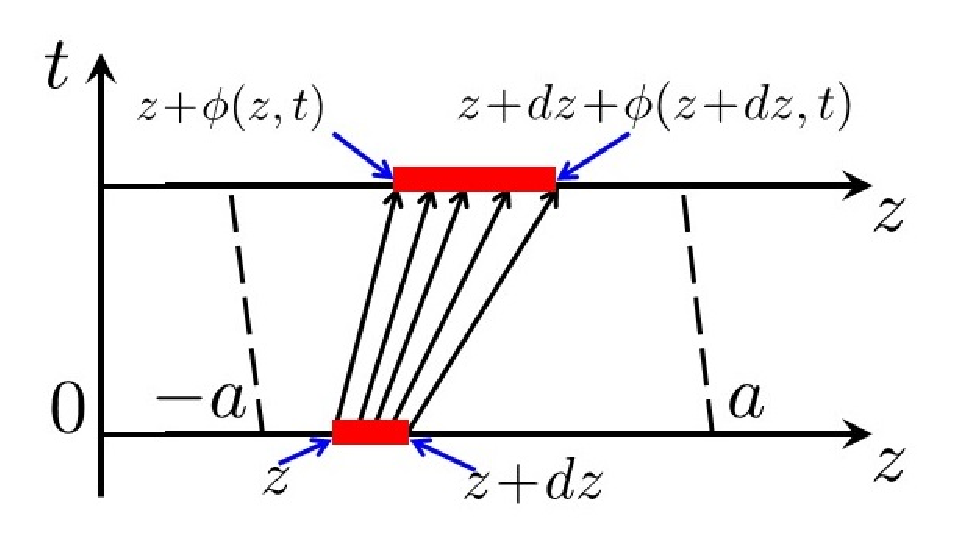
\includegraphics[width=0.5\columnwidth]{displacement_2}
\caption{(color online)
The definition of the displacement field $\phi(z,t)$ in Lagrangian formulation. 
At the time, shown as vertical axis, $t=0$ the fluid is contained in the interval $|z|<a$.
As time progresses the particles of a fluid move as indicated by narrow arrows pointing upward.
The particle located at $z$ at $t=0$ is shifted to the new position $z+\phi(z,t)$. 
A fluid volume shown as a narrow (red) horizontal rectangle occupies a segment $[z,z+dz]$ at time $t=0$.
At a later time $t>0$ this volume is displaced and occupies the segment $[z+\phi(z,t),z+dz+\phi(z+dz,t)]$.
The fluid volume expands (shrinks) if $\partial \phi(z,t)/ \partial z > (<) 0$.
The expansion (shrinkage) translates in the decrease (increase) in the density respectively.\cite{Iqbal2}}
\label{Fig-phi}
\end{centering}
\end{figure}


It should be noted that this segment is from $z$ to $z + d z$ in Lagrangian coordinates.
The force due to the pressure gradient is
\be\label{F_P}
F_P = P'(z + \phi(z,t)) - P'(z + d z + \phi(z + d z,t))
\ee
We assume that the pressure is the function of the density.
Then according to \eqref{hydro1} 
\be
P'(z+ \phi(z,t)) = P ( n'(z + \phi(z,t))) = P( \frac{ n(z) }{ 1 + \partial_z \phi(z,t)})
\ee
By the same token,
\be
P'(z+d z + \phi(z + dz,t)) = P ( n'(z+dz + \phi(z+dz,t))) = P( \frac{ n(z+dz) }{ 1 + \partial_z \phi(z+dz,t)})
\ee
Therefore the force is
\be
F_{P} = - \partial_z P(\frac{n(z)}{1 + \partial_z \phi(z,t)}) d z
\ee

\subsection{Force Due to the Confinement Potential}

The force due to the confinement potential, $U(z)$ exerted on the segment occupying the strip from $z$ to $z + dz$ in Lagrangian coordinates is 
\be
F_c = - \partial_z U(z + \phi(z,t)) n'(z + \phi(z,t)) d z = - \partial_z U(z + \phi(z,t)) n(z) d z
\ee

\subsection{Viscous Forces}

These forces conserve the total momentum, but roughly cause its diffusion.
Consider again the same parcel of a fluid.
The net force due to the viscosity in the leading in $\phi$ approximation reads
\be
\begin{split}
\label{vis_force}
- \eta(z+dz + \phi(z + dz)) \partial_z v[ z+dz + \phi(z + dz)] + 
\eta(z+ \phi(z )) \partial_z v[ z + \phi(z)] \\
\approx 
- 
\partial_z [\rho(z) \mu(z) \partial_z \partial_t \phi(z,t)]
\end{split}
\ee
Here we denote by $\eta(z)$ dynamic viscosity and $\mu(z) = \eta(z) / \rho(z)$ the kinematic viscosity.






\subsection{Newton's Law for Ideal fluid}
The acceleration of this same segment of fluid is
\be
a(z,t) = \partial^2_t \phi(z,t)
\ee

For a given parcel of a fluid  of a mass $n(z) m d z$, the Newton Law gives,
\be
m n(z) \partial_t^2 \phi(z,t) = - \partial_x P( \frac{ n(z) }{ 1 + \partial_z \phi(z,t)} ) - \partial_z U(z + \phi(z,t)) n(z)
\ee
This equation is exact. Linearizing in the displacement field $\phi$ we get,
\be
n(z,t) \approx n(z) - n(z) \partial_z \phi(z,t)
\ee
%\be
%P( \frac{ n(z) }{ 1 + \partial_z \phi(z,t)} ) \approx P ( n(z) - n(z) \partial_z \phi(z,t)) \approx P(n(z)) - \frac{\partial P(n(z))}{\partial n(z)} n(z) \partial_z \phi
%\ee
%\be
%\partial_z U(z + \phi(z,t)) n(z) \approx \partial_z U(z) n(z) + \partial^2_z U(z) n(z) \phi(z,t)
%\ee
The linearized equation of motion is given by:
\begin{align}
\label{hydro39}
&m n(z) \partial_t^2 \phi(z,t) = \notag \\
&-\partial_z P(n(z)) + \partial_z \left[  \frac{\partial P(n(z))}{\partial n(z)} n(z) \partial_z \phi(z,t)\right]
-\partial_z U(z) n(z) - \partial^2_z U(z) n(z) \phi(z,t)
\end{align}
At equilibrium we must get,
\be\label{hydro41}
0 = -\partial_z P(n(z)) -\partial_z U(z) n(z) = - \frac{ \partial P(n)}{\partial n } \frac{ \partial n(z) }{\partial z} - \partial_z U(z) n(z)
\ee

%We can write \eqref{hydro39} as
%\be\label{hydro47}
%m n(z) \partial_t^2 \phi(z,t) = 
%\partial_z \left[  \frac{\partial P(n(z))}{\partial n(z)} n(z) \partial_z \phi(z,t)\right]
% - \partial^2_z U(z) n(z) \phi(z,t)
%\ee
%Rewrite the second term as
%\be\label{hydro49}
%\partial_z \left[  \frac{\partial P(n(z))}{\partial n(z)} n(z) \partial_z \phi(z,t)\right]
%=
%n(z) \partial_z \left[  \frac{\partial P(n(z))}{\partial n(z)}  \partial_z \phi(z,t)\right]
%+ 
% \left[ \partial_z n(z) \right] \frac{\partial P(n(z))}{\partial n(z)} \partial_z \phi(z,t)
%\ee
%Using \eqref{hydro41}, \eqref{hydro49} becomes 
%\be\label{hydro51}
%\partial_z \left[  \frac{\partial P(n(z))}{\partial n(z)} n(z) \partial_z \phi(z,t)\right]
%=
%n(z) \partial_z \left[  \frac{\partial P(n(z))}{\partial n(z)}  \partial_z \phi(z,t)\right]
%-\partial_z U(z) n(z)  \partial_z \phi(z,t)
%\ee
%Substituting \eqref{hydro51} in \eqref{hydro39} allows to rewrite \eqref{hydro39} after canceling the equilibrium density $n(z)$ as
%\be\label{hydro53}
%m \partial_t^2 \phi(z,t) = 
%\partial_z \left[  \frac{\partial P(n(z))}{\partial n(z)}  \partial_z \phi(z,t)\right]
%-\partial_z U(z)  \partial_z \phi(z,t)
% - \partial^2_z U(z) \phi(z,t)
%\ee
After applying the equilibrium condition, equation \eqref{hydro39} can be rewritten as
\be\label{hydro55}
 \partial_t^2 \phi(z,t) = 
\partial_z \left[  \frac{\partial P(\rho(z))}{\partial \rho(z)}  \partial_z \phi(z,t)\right]
-\partial_z U_c(z)  \partial_z \phi(z,t)
 - \partial^2_z U_c(z) \phi(z,t)
\ee
The mass density, $\rho(z) = m n(z)$ and the partial derivative of the pressure in the right hand side of \eqref{hydro55} is understood as adiabatic as the fluid is assumed to be ideal.
We therefore define the local speed of sound as
\be
v_s^2 = \frac{\partial P(\rho(z))}{\partial \rho(z)} 
\ee
and look for the solutions in the form,
\be
\phi(z,t) = e^{- i \omega t } \phi(z)
\ee
so we get from \eqref{hydro55}
\be\label{hydro63}
 \omega^2 \phi(z) = 
- \partial_z \left[ v_s^2( n(z))  \partial_z \phi(z)\right]
+\partial_z U_c(z)  \partial_z \phi(z)
 + \partial^2_z U_c(z) \phi(z)
\ee

We consider a velocity Potential, $\chi(z)$ satisfying $\phi(z) = \chi'(z) = d\chi/ d z$.
With this potential \eqref{hydro63} takes the form,
\be\label{hydro65}
 \omega^2 \chi'(z) = 
- \partial_z \left[ v_s^2( n(z)) \chi''\right]
+\partial_z U_c(z)  \chi''
 + \partial^2_z U_c(z) \chi'
 =
 \partial_z \left[ - v_s^2( n(z)) \chi''  + \partial_z U_c(z)\chi' \right]
\ee
After removing one derivative by integration back over $z$ we get,
\be\label{hydro67}
 \omega^2 \chi + v_s^2( n(z)) \chi''-\partial_z U_c(z)  \chi'
 =0
\ee
\section{Exactly Solvable Cases}
Here we point out some solutions of linearized equation of an ideal fluid that are relevant for us.
\subsection{Kohn Mode in Hydrodynamics}
If we have a parabolic confinement potential $U_c = \omega_{\perp}^2 \frac{z^2 }{2}$, we get for the Euler equation,
\be\label{hydro69}
 \omega^2 \chi + v_s^2( n(z)) \chi''-\omega_{\perp}^2 z \chi'
 =0
\ee
The Kohn mode is then given by $\chi = \alpha z$ with $\omega = \omega_{\perp}$ regardless of the functional form of the sound velocity, $v_s^2$
%\subsection{Extended System, $\mathrm{U_c = const}$}
For an extended system with the confinement potential, $\mathrm{U_c = const}$, we just get the wave equation,
\be\label{hydro71}
 \omega^2 \chi + v_s^2 \chi'' =0
\ee
as it should be for linearized hydrodynamics of compressible and ideal fluid.
\subsection{Free Degenerate 2D Ideal Fermi Gas at $T=0$ in Parabolic Well}
This is the limit of primary interest to us.
Strictly speaking the hydrodynamics requires collisions and we assume that from the point of view of collisions our gas is not ideal.
But the Fermi liquid renormalizations are neglected here.
Spin is ignored too.

Let us fix the Fermi energy, $E_F$.
Then the maximal kinetic energy is reached at the center of the channel, and the gas occupies the strip of a width $2a$, where
\be\label{hydro77}
a =  \sqrt{ \frac{2 E_F}{ m \omega_{\perp}^2}}\, .
\ee
We therefore have for our gas from \eqref{hydro69} and \eqref{hydro75}
\be\label{hydro91}
 \omega^2 \chi + \frac{ \omega_{\perp}^2 }{2} (a^2 -z^2) \chi''-\omega_{\perp}^2 z \chi'
 =0
\ee
Now redefine the length scale $z \rightarrow z/a$,  multiply by $2/\omega_{\perp}^2$ and define
\be\label{hydro93}
\lambda_{\omega}^2 =2 \frac{\omega^2}{\omega_{\perp}^2 }
\ee
This makes \eqref{hydro91} to look as the Legendre equation,
\be\label{hydro91a}
 \lambda_{\omega}^2 \chi + (1 -z^2) \chi''-2 z \chi'
 =0
\ee
we therefore read off the solutions.
\be\label{hydro94}
\lambda_{\omega_n}^2 = 2 \frac{\omega_n^2}{\omega_{\perp}^2 } = n(n+1)
\ee
with $n=0,1,...$
so that the frequencies are
\be\label{hydro95}
\omega_n = \omega_{\perp} \sqrt{ \frac{ n(n+1)}{2}}
\ee
$n=0$ gives a ground state since as $\chi = const$, the velocity is identically zero.
$n=1$ is a Kohn mode as $P_1(z) = z$ is indeed linear.
We were able to get the whole hierarchy  of eigenoscilations of an electronic weakly interacting liquid.
They are Legendre polynomials,
\be
\chi_n(z/a) = \sqrt{\frac{ 2 n +1}{2}}P_n(z/a)
\ee
and the velocity fields are
\be
v_n(z/a) =   \partial_z P_n(z/a)\, .
\ee
\section{Depolarization Shift for the Kohn Mode in Ideal Fluid with Finite Non-Parabolicity}
We consider a weak anharmonicity,
\be\label{hydro96}
U_c(z) = \omega_{\perp}^2 \frac{z^2 }{2} + \frac{\epsilon}{4 m} z^4 + \delta U_c
\ee
where the constant $\delta U_c \propto \epsilon $ is added  in such a way that the spatial extent of the electronic liquid stays the same as for $\epsilon =0$.
In other words, 
\be
\delta U_c + \frac{\epsilon}{4 m} a^4 = 0
\ee
This is in fact not necessary, but convenient.
The convenience achieved this way is the absence of 
$\delta$-function contribution to the density, $\delta \rho \propto \delta(z \pm a)$.
We reconsider the Euler equation, \eqref{hydro67}.
It requires two modifications.
The first modification comes from the third term which becomes now according to \eqref{hydro96},
\be\label{hydro97}
-\partial_z U_c(z)  \chi' = \omega_{\perp}^2 z  + \frac{\epsilon}{ m} z^3\, .
\ee
The second modification is due to the change in the speed of sound which now reads
\begin{align}\label{hydro98}
v_s^2(z) & = \frac{1}{2} v_F^2(z) = \frac{1 }{ m } E_F(z) = 
\frac{1}{m} (E_F - \frac{ k z^2 }{2} - \frac{\epsilon}{4} z^4 - \delta U_c ) 
\notag \\
& =
\frac{k}{ 2 m} (a^2 - z^2- \frac{\epsilon}{2 m \omega_{\perp}^2} z^4+\frac{\epsilon}{2 m \omega_{\perp}^2} a^4) = \frac{ \omega_{\perp}^2 }{2} (a^2 -z^2) -
\frac{ \omega_{\perp}^2 }{2} \frac{\epsilon}{2 m \omega_{\perp}^2} (z^4 - a^4)
\end{align}
As a result the second term of \eqref{hydro67} takes the form,
\begin{align}
v_{s}^2 \chi'' = \frac{ \omega_{\perp}^2 }{2} (a^2 -z^2)\chi'' -
\frac{ \omega_{\perp}^2 }{2} \frac{\epsilon}{2 m \omega_{\perp}^2} (z^4-a^4) \chi''
\end{align}
Finally instead of the rescaled equation \eqref{hydro91} we obtain a modified equation,
\be\label{hydro101}
 \lambda_{\omega}^2 \chi + (1 -z^2) \chi''  -2 z \chi' 
 -
 \frac{\epsilon a^2 }{2 m \omega_{\perp}^2} (z^4 - 1) \chi''
 - \frac{2 a^2 \epsilon}{m \omega_{\perp}^2} z^3 \chi' 
 =0
\ee
We present it in the form,
\be\label{hydro101a}
 \lambda_{\omega}^2 \chi + (1 -z^2) \chi''  -2 z \chi' 
+V_{pert}^{\epsilon} [\chi] =0
 \ee
 where the perturbation reads
 \be\label{hydro101b}
 V_{pert}^{\epsilon} [\chi] = 
 -\frac{\epsilon a^2 }{2 m \omega_{\perp}^2}
 ( (z^4 - 1) \partial_z^2+  4 z^3 \partial_z )\chi =
  -\frac{\epsilon a^2 }{2 m \omega_{\perp}^2}
\partial_z[  ( (z^4-1) \partial_z )\chi]
\ee
It is absolutely crucial that $V_{pert}^{\epsilon}$ is Hermitian.
It follows from the simple observation that the anharmonicity alone causes the frequency shift but not a dissipation of the eigenmodes.
It also holds for any anharmonicity, 
% after the change, 
%$\partial_z[(z^4 -1)\partial_z \chi(z)] \rightarrow  \partial_z[(U_c^{anhar}(z) - U_c^{anhar}(a))\partial_z \chi(z)]$.
and in principle all the results on shift are generalizable to any anharmonic potential. 

It is crucial that the addition of $\delta U_c$ in \eqref{hydro96} modifies neither these conclusions  nor the final results.
Without this term thing would get messy because of the $\delta$-functions added to the density as described above.

To the leading order in $\epsilon$ we write,
\be
\lambda^2_{\omega_1} = 2 + \delta \lambda_1^2
\ee
where 
\be
\delta \lambda^2 = 2 \frac{\epsilon}{m \omega_{\perp}^2} 
\frac{ 2 *1 +1}{ 2 } a^2 \langle P_1(z)|\frac{1}{4} (z^4-1) \partial_z^2 + z^3 \partial_z| P_1(z)\rangle
\ee
here, dimensions were restored, and $a$ defined by \eqref{hydro77} is the size of the fermion cloud.
We now notice that
\be
\langle P_1(z)| \frac{1}{4} (z^4-1) \partial_z^2 + z^3 \partial_z| P_1(z)\rangle = \frac{2}{5}
\ee
so that
\be
\delta \lambda_1^2 = 2 \frac{\epsilon a^2}{m \omega_{\perp}^2} 
\frac{ 3}{ 2 }\frac{2}{5} = 
\frac{ 6 a^2}{5}\frac{\epsilon}{m \omega_{\perp}^2} 
\ee
Therefore
\be
2 \frac{\omega^2_1 }{ \omega_{\perp}^2} \approx 2 + \frac{ 6 a^2 }{5}\frac{\epsilon}{m \omega_{\perp}^2} 
\ee
and the correction to the Kohn mode frequency, $\delta \omega_1$ to the leading order in anharmonicity is
\be\label{hydro149}
\boxed{\frac{\delta \omega_1}{\omega_{\perp}} = \frac{ 3}{10}\frac{\epsilon a^2}{m \omega_{\perp}^2} }
\ee
We can also write it more explicitly using \eqref{hydro77} as 
\be
\boxed{\frac{\delta \omega_1}{\omega_{\perp}} = \frac{ 3}{5}\frac{ \epsilon E_F}{ (m \omega_{\perp}^2)^2} }
\ee

It can be explicitly verified that this result agrees with what one would get following the approach of \cite{Pantel2012}.


\section{Viscosity: Normal Modes Dissipation}
Here we analyze how the normal modes we found before get a finite relaxation time due to the processes of internal friction, i.e. the viscosity.
And start with the equation \eqref{hydro39} modified to include the viscous force, Eq.~\eqref{vis_force},
\begin{align}
\label{V14}
m n(z) &\partial_t^2 \phi(z,t) = \notag \\
 &\partial_z \left[  \frac{\partial P(n(z))}{\partial n(z)} n(z) \partial_z \phi(z,t)\right] - \partial^2_z U(z) n(z) \phi(z,t) - 
\partial_z [\rho(z) \mu(z) \partial_z \partial_t \phi(z,t)]
\end{align}
In terms of the velocity potential, we get instead of \eqref{hydro65}, %and assuming a constant $\eta$,
\be\label{V15}
 \omega^2 \chi'(z) = 
 \partial_z \left[ - v_s^2( n(z)) \chi''  + \partial_z U_c(z)\chi' \right]
 -
 i \omega  \frac{1}{  n(z)} \partial_z ( \mu(z) n(z) \partial_z^2 \chi(z))
\ee
 Integration over $z$ gives
 \be\label{V15}
 \omega^2 \chi(z) = 
 \left[ - v_s^2( n(z)) \chi''  + \partial_z U_c(z)\chi' \right]
 -
 i \omega \int_b^z \frac{d z }{  n(z)} \partial_z (\mu(z) n(z) \partial_z^2 \chi(z))
\ee
where the lower limit of the integral, $b$ is arbitrary.
It will be important to show that the final results are not dependent on $b$. 
We now make the same manipulations leading to Eqs.~\eqref{hydro101a} and \eqref{hydro101b} in Eq.~\eqref{V15}
\be\label{hydro101a}
 \lambda_{\omega}^2 \chi + (1 -z^2) \chi''  -2 z \chi' 
+V_{pert}^{\epsilon} [\chi] + V_{pert}^{\eta} [\chi] =0
 \ee
where the perturbation, $V^{\epsilon}_{pert}$ is defined by Eq.~\eqref{hydro101b}, and 
\be\label{V301}
V_{pert}^{\eta} [\chi] =  -
 i \omega \frac{2 \mu_0 }{ a^2 \omega_{\perp}^2} \int_b^z \frac{d z }{  n(z)} \partial_z (\bar{\mu}(z) n(z) \partial_z^2 \chi(z))
\ee
where $\mu_0 = \mu(z=0)$, and $\bar{\mu}(z) = \mu(z)/\mu_0$.
The exact $z$-dependence of $\mu(z)$ is not essential, and changes the numbers in finite results.
For the Fermi liquid $\eta \propto \rho v_F \ell$, $\ell \propto v_F E_F/T^2$,
\be\label{na}
\mu = \eta/\rho \propto  v_F^2 E_F/ T^2 = C_{\mu} n^2/(m^3 T^2) 
\ee
from \eqref{na} with $C_{\mu}>0$ a numerical constant.
It follows that 
\be\label{FL_mu}
\mu_0 = C_{\mu} \frac{ n^2(z=0)}{ m^3 T^2}\, ,\quad \bar{\mu}(z) = (1-z^2)^2
\ee
Using the definition, \eqref{hydro94} and introducing a constant 
\be
B =  \frac{\sqrt{2} \mu_0 }{ a^2 \omega_{\perp}} 
\ee
we put \eqref{V301} in the form 
\be\label{V301}
V_{pert}^{\eta} [\chi] =  -
 i \lambda_{\omega} B \int_b^z \frac{d z }{  n(z)} \partial_z (\bar{\mu}(z) n(z) \partial_z^2 \chi(z))
 =
 -
 i \lambda_{\omega} B \int_b^z \frac{d z }{ 1-z^2} \partial_z [(1-z^2)^3 \partial_z^2 \chi(z)]
\ee
\subsubsection{Perturbation Theory: Kohn Mode
% to Order $ \epsilon^0 \eta^n$ with Arbitrary $n=1,2,\ldots$
}
For the order of $ \epsilon^0 \eta^n$ with Arbitrary $n=1,2,\ldots$, we note that the Kohn mode is unaffected by viscosity at $\epsilon=0$, to any order in viscosity since,
\be\label{V303}
V_{pert}^{\eta} [\chi_1] =0
\ee
as expected from the Galilean invariance. Now we will investigate what happens at finite $\epsilon$.

%\subsubsection{Perturbation theory: Kohn mode to order $\epsilon^1 \eta^n$ with arbitrary $n=1,2,\ldots$}

We consider first $\epsilon^1 \eta^1$ order.
We know that the Kohn mode is shifted in frequency and at the same time acquires a finite admixture of the higher modes.
To the order $\epsilon \eta$ we have the following correction to $\lambda_{\omega_1}$,
\begin{align}
\label{V307}
\delta \lambda^2_1 = - i \lambda_{\omega} B  \sum_{n=1}^{\infty}& 
\frac{\sqrt{ 3/2 }\sqrt{(2 n +1)/2}}{2 - n(n+1)} \notag \\
&\left[
\langle P_1| V_{pert}^{\eta} | P_n\rangle \langle P_n| V_{pert}^{\epsilon} | P_1 \rangle
+
\langle P_1| V_{pert}^{\epsilon} | P_n\rangle \langle P_n| V_{pert}^{\eta} | P_1 \rangle \right]
\end{align}
Among the two terms in \eqref{V307} the second vanishes according to \eqref{V303}.
The first term vanishes as well,
\begin{align}
\langle P_1| V_{pert}^{\eta} | P_n\rangle & \propto
\int_{-1}^{1} d x P_1(x) \int_{b}^x d z \frac{1}{n(z)} \partial_z(n^3(z) \partial^2_z P_n(z)
\notag \\
&=\frac{1}{2} \int_{-1}^{1} d x \partial_x n(x) \int_{b}^x d z \frac{1}{n(z)} \partial_z [n(z)^3 \partial^2_z P_n(z)]
\notag \\
&=
-\frac{1}{2} \int_{-1}^{1} d x n(x)  \frac{1}{n(x)} \partial_x [n^3(x) \partial^2_z P_n(x)]
\notag \\
&=
-\frac{1}{2} \int_{-1}^{1} d x  \partial_x [n^3(x) \partial^2_x P_n(x)]
=0
\end{align}
regardless of $b$ and $n$.
It may be noted that the cancellation is not specific to the model of viscosity, it will hold as long as $\eta=0$ in the limit of $\rho =0$ which is quite natural: in the absence of particles there no carriers of momentum.
It follows that the correction to the frequency vanishes to any order to $\epsilon \eta^n$ with $n=1,2,\ldots$.



This is an important observation, as in the case we had a finite result, the new energies would be found from $\omega_1^2 = 2 + i \eta \epsilon \omega_1 $ which gives the imaginary part to $\omega_1$ that has the sign determined by the sign of $\epsilon$ which is an impossible conclusion.

%\subsubsection{Perturbation theory: Kohn mode to order $\epsilon^2 \eta^1$.} 
The leading non-vanishing correction comes from the order $\epsilon^2 \eta^1$ term.
According to the perturbation theory the third order correction is given by 
\begin{align}
\delta E^{(3)}_0 = \sum_{k \neq 0}\sum_{m \neq 0} \frac{ \langle 0 | V |m \rangle \langle m | V | k \rangle \langle k  | V | 0\rangle}
{(E_m - E_0)(E_k - E_0)}
-
\langle 0 | V | 0 \rangle  \sum_{m \neq 0} \frac{ \langle 0| V | m\rangle  \langle m| V | 0 \rangle}{ (E_m - E_0)^2 } 
\end{align}
Identifying $|0\rangle = | P_1 \rangle$ as a Kohn mode, and $V = V_{pert}^{\eta} + V_{pert}^{\epsilon}$ and noting that in general
\be
\langle P_1 | V_{pert}^{\eta} | P_n \rangle = \langle P_n | V_{pert}^{\eta} | P_1 \rangle = \langle P_1 | V_{pert}^{\epsilon} | P_1 \rangle = 0, \mathrm{for\, all}\, n
\ee
and for quartic anharmonicity in particular the only non-zero off-diagonal matrix elements are, using \eqref{hydro101b} is $\langle P_1 | V_{pert}^{\epsilon} | P_3 \rangle = \langle P_3 | V_{pert}^{\epsilon} | P_1 \rangle$ with the rest of the matrix elements $\langle P_n | V_{pert}^{\epsilon} | P_1 \rangle =0 $ for $n\neq 1,3$.
We thus have, including the normalization factors,
\be
\delta^{(3)} \lambda_{\omega_1}^2 = \frac{ \langle   P_1| V_{pert}^{\epsilon} | P_3 \rangle \langle  P_3 | V_{pert}^{\eta} | P_3 \rangle \langle P_3 |V_{pert}^{\epsilon} | P_1 \rangle }{ (\lambda_1^2 - \lambda_3^2)^2} \frac{ 2 *1 + 1}{2} \left(\frac{2*3 + 1}{2}\right)^2
\ee
where $\lambda_1^2 = 1(1+1)=2$ and $\lambda_3^2 = 3(3+1)=12$ 
and  $(\lambda_1^2 - \lambda_3^2)^2 = 10^2$.
Using the explicit expressions  \eqref{V301}, \eqref{hydro101b} , and the numbers,
\begin{align}
\label{PT101}
 \int_{-1}^1 d z P_3(z) \int_b^z \frac{d x }{ 1-x^2} \partial_x [(1-x^2)^3 \partial_x^2 P_3(x)] &= - \frac{40}{21}\notag \\
 \int_{-1}^1 d z P_1(z) \partial_z [(z^4 - 1)\partial_z P_3(z)] &= \frac{8}{5}
\end{align}
along with the definition \eqref{hydro93}
\begin{align}
\delta^{(3)} \lambda_{\omega_1}^2 = 
\delta^{(3)} 2 \frac{\omega^2}{ \omega_{\perp}^2} =
- i \lambda_{\omega} \frac{\sqrt{2} \mu_0 }{ a^2 \omega_{\perp}} \left(\frac{\epsilon a^2 }{2 m \omega_{\perp}^2}\right)^2 ( - \frac{40}{21}) \left(\frac{8}{5}\right)^2 \frac{3}{2} (\frac{7}{2})^2 10^{-2}
\end{align}
For now omitting the numerical prefectures we get
\begin{align}
\frac{\delta \omega}{\omega_{\perp}} = i \frac{\mu_0 }{ a^2 \omega_{\perp}} 
\left(\frac{\epsilon a^2 }{ m \omega_{\perp}^2}\right)^2 
= i \frac{ \mu_0 \epsilon^2 a^2 }{m^2 \omega_{\perp}^5}
\end{align}
The relaxation rate for the mode,
is 
\begin{align}
\boxed{\frac{1}{\tau_{Kohn}} \propto \frac{ \mu_0 \epsilon^2 a^2 }{m^2 \omega_{\perp}^4}}
%= \frac{  \epsilon^2 a^4 }{m^2 \omega_{\perp}^4} \frac{\mu_0}{a^2}
\end{align}
To interpret this result we use the expression \eqref{hydro149} to write it in the form,
\begin{align}\label{res_life}
\boxed{\frac{1}{\tau_{Kohn}} \propto \left(\frac{ \delta \omega_1}{\omega_{\perp}} \right)^2 \frac{\mu_0}{a^2}}
\end{align}
which has a straightforward interpretation.
The higher modes not protected by the Kohn theorem decay with the rate,
$ \mu_0 / a^2 $ as $\mu_0$ has dimensions of the diffusion coefficient.
This is the typical rate of momentum relaxation. 
The ratio  $\left(\frac{ \delta \omega_1}{\omega_{\perp}} \right)^2$ is the probability of finding the system in higher modes.

\section{Solution of Navier-Stokes equations}
A hydrodynamic description is based on the existence of slow variables associated with locally conserved quantities such as number of particles, momentum and energy. The motion of the liquid is described by the Navier-Stokes equations which in Eulerian continuous field coordinates can be put in the form~\cite{LL} 
\begin{equation}\label{E-eq}
\partial_t(\rho v_j)=-\partial_i\Pi_{ij}-\rho\partial_jU,
\end{equation}
that guaranties the momentum conservation, which holds in ideal and nonideal liquids alike in the absence of confining potential $U$. The stress tensor of a two-dimensional fluid giving rise to the Navier-Stokes equation is~\cite{LL} 
\begin{equation}\label{Pi}
\Pi_{ij}=\delta_{ij}P+\rho v_iv_j-\zeta\delta_{ij}\partial_kv_k
-\eta(\partial_iv_j+\partial_jv_i-\delta_{ij}\partial_kv_k).
\end{equation}
Here $\eta,\zeta$ are the first (shear) and second (bulk) viscosities, and $P$ is pressure. In the following we focus on a one-dimensional flow in $z$-direction of a two-dimensional liquid occupying the strip $|z|<a$, so that velocity vector field can be taken in the form $\bm{v}=v(z,t)\bm{e}_z$ and Eq.~(\ref{E-eq}) simplifies to 
\begin{equation}\label{NS-eq}
\rho(\partial_t v+v\partial_zv)=-\partial_z P-\rho \partial_z U+\partial_z(\eta\partial_zv).
\end{equation}  
When writing this equation we made use of the continuity equation $\partial_t\rho+\partial_z(\rho v)=0$ and employed standard assumption $\eta\gg\zeta$. For the purpose of our study it will be convenient to use a particle description of Navier-Stokes equation.
In this approach the coordinate $z$ labels an equilibrium position of a fluid particle, and its location at later time $t$ is the $z+ \phi(z,t)$ such that $\phi$ is the displacement field.
By definition, the density is $\rho(z+\phi(z,t),t) = \rho_0(z)/ ( 1 + \partial_z \phi(z,t))$, the velocity $v(z+\phi(z,t)) = \partial_t \phi(z,t)$.
The linearization of Eq.~\eqref{NS-eq} is equivalent to the linearization in $\phi$.
To the leading order, 
\begin{align}\label{leading}
\rho = \rho_0 + \delta \rho\, ,\,\, \delta \rho  = 
- (\rho_0 \phi)'  \, , \quad  v = \dot{\phi} \, ,
\end{align}
where $\rho_0$ is a stationary equilibrium density distribution, the notations $f' = \partial f/ \partial z$ and $\dot{f} = \partial f / \partial t$ are introduced and the pair of arguments $(z,t)$ common to all the functions is omitted.  
The parametrization \eqref{leading} of $\delta \rho$ and $v$ by a single displacement field automatically satisfies the linearized continuity equation, $\delta \dot{\rho} + (\rho_0 \dot{\phi})' = 0$.
The concept of the displacement field is further illustrated in Fig.~\ref{Fig-phi}. For the solutions of the form $\phi(z,t) = e^{i \omega t} \chi'(z)$ the equation \eqref{NS-eq} in the parameterization, \eqref{leading} reads, (see Appendix \ref{App2}):
\begin{equation}\label{normal-modes-eq}
\omega^2\chi=-v^2_s\chi''+U'\chi' -i\omega\int^{z}_{z_0}\frac{dz}{\rho_0}(\nu \rho_0 \chi'')',
\end{equation}
where $\nu(z)=\eta(z)/\rho_0(z)$ is the kinematic viscosity, and
\begin{align}\label{v_s}
v_s=\sqrt{\partial P/\partial\rho_0}
\end{align}
has a meaning of a local speed of sound that depends on $z$ only through the equilibrium density $\rho_0$. We show that the results are independent on arbitrary $z_0$.

The spectrum of collective excitations and their decay rates as given by Eq.~\eqref{normal-modes-eq} depend on the details of the confining potential and dependence of the viscosity on density. 
Here for definiteness we consider the confining potential per unit mass with a weak quartic anharmonicity,
\begin{equation}\label{U}
U=\frac{\omega^2_\perp z^2}{2}+\frac{\epsilon z^4}{4m}+\delta U,
\end{equation}
where $m$ is the mass of an individual particles, and the constant $\delta U\propto\epsilon$ is added in such a way that the spatial extent of the liquid stays the same as for $\epsilon=0$. In other words $\delta U+\epsilon a^4/4m=0$. This choice is not obligatory, yet convenient in the further calculations. 
The anharmonic part $\propto\epsilon$ of $U$ not only modifies the second term in the right-hand-side of Eq.~(\ref{normal-modes-eq}) but also the first one. Indeed, in the parabolic confinement the sound velocity is $v^2_s(z)=2\pi \rho(z)/m^3=\omega^2_\perp(a^2-z^2)/2$, which acquires now a correction $\delta v^2_s(z)=-\epsilon(z^4-a^4)/4m$.  
With these observations in mind we multiply Eq.~(\ref{normal-modes-eq}) by $2/\omega^2_\perp$, rescale coordinates $z\to z/a$ and introduce $\lambda^2_\omega=2\omega^2/\omega^2_\perp$ to find 
\begin{equation}\label{eigenmodes}
\lambda^2_\omega\chi+(1-z^2)\chi''-2z\chi'+V_\epsilon+V_\nu=0.
\end{equation}
The perturbation term due to anharmonicity can be cast in the form 
\begin{equation}\label{V1}
V_\epsilon=-\frac{\epsilon a^2}{2m\omega^2_\perp}[ (z^4-1)\chi ']'.
\end{equation}
This formula can be generalized to any confining potential after the change $[(z^4-1)\chi']'\to [(U(z)-U(a))\chi']'$. Consequently, our results for the depolarization shift are straightforward to modify for arbitrary confinements. 
We emphasize that $V_\epsilon$ is Hermitian. 
This property guaranties that the anharmonicity alone causes only the frequency shift but no dissipation. We argue below that only the combination of the anharmonicity and viscosity leads to the dissipation of the Kohn mode. The exact $z$-dependence of the viscosity $\nu(z)$ is specific to the model. This however only influences the numerical prefactors in the final results and we take the expression for the viscosity from the theory of Fermi liquids, $\eta\propto v_F\rho\ell$, where mean fee path is $\ell\propto v_FE_F/T^2$ with $v_F$ and $E_F$ being Fermi velocity and energy, respectively. 
For this case $\nu(z)=C\rho^2(z)/m^5T^2$ where $C$ is the numerical factor of the order of unity~\cite{Abrikosov}. In the above specified dimensionless notations this results in 
\begin{equation}\label{V2}
V_\nu=-i\lambda_\omega B\int^{z}_{z_0}\frac{dz}{1-z^2}[(1-z^2)^3  \chi'']',
\end{equation}
where we have introduced $B=\sqrt{2}\nu_0/a^2\omega_\perp$ with $\nu_0=\nu(z=0)$. We proceed with the analysis of Eq.~(\ref{eigenmodes}). 

\section{Results}
As the first step let us discuss the eigenmodes of an ideal fluid confined to a harmonic trap. For that purpose we neglect anharmonicity and interaction effects implicit in the viscosity term of Eq.~(\ref{eigenmodes}), i.e. we set $V_{\epsilon} =V_{\eta}=0$. 
What remains is familiar Legendre equation and we therefore immediately read off its solutions $\lambda^2_{\omega_n}=2\omega^2_n/\omega_\perp=n(n+1)$ with $n=0,1,2,\ldots$ so that the eigenfrequencies are 
\begin{equation}\label{omega-n}
 \omega_n=\omega_\perp\sqrt{\frac{n(n+1)}{2}}. 
\end{equation}
The $n=0$ gives an equilibrium since $\chi_{n=0}=const$ this velocity is identically zero. The $n=1$ is a Kohn mode $\omega_1=\omega_\perp$. We thus found the whole hierarchy of eigenoscillations, they are Legendre polynomials 
\begin{equation}\label{chi}
\chi_n(z)=\sqrt{\frac{2n+1}{2}}P_n(z)
\end{equation} 
and the related velocity fields are $v_n(z)=\partial_zP_n$. 
Remarkably, the same spectrum of collective modes as \eqref{omega-n} was obtained recently for the longitudinal oscillations of the one-dimensional Coulomb chains \cite{Morigi_PRE}.
In this systems the collective behavior sets in due to the long range Coulomb forces rather than collisions.

Next we discuss the significance of perturbation terms on the spectrum of collective modes. Let us first consider anharmonicity alone, i.e. we set $V_{\eta}=0$ and $V_{\epsilon}\neq 0$ in Eq.~\eqref{eigenmodes}. As $V_{\epsilon}$ is Hermitian the spectrum remains real.
As a result all the eigenmodes remain undamped as expected in the absence of collisions.
To find the depolarization shift of the Kohn mode, $\delta^{(1)} \omega_1$ to the leading order in $\epsilon$ we write $\lambda^2_{\omega_1}=2+\delta^{(1)} \lambda^2_{\omega_1}$, where the correction term is found from the first order perturbation theory 
\begin{equation}
\delta^{(1)} \lambda^2_{\omega_1}=\frac{3\epsilon a^2}{4m\omega^2_\perp}\langle P_1(z)|(z^4-1)\partial^2_z+4z^3\partial_z|P_1(z)\rangle.
\end{equation}
The matrix element gives a factor of $8/5$ which eventually translates into the correction to the Kohn mode frequency 
\begin{equation}\label{dep_shift}
\delta^{(1)}\omega_1=\frac{3\epsilon a^2}{10m\omega_\perp}.
\end{equation}
We have checked that the result \eqref{dep_shift} agrees with the result obtained by the method of moments suggested in Ref.~\cite{Pantel2012}. We note however that the result for the depolarization shift in the collisioneless regime differ from Eq.~\eqref{dep_shift} by a nonuniversal numerical prefactor. 
For instance, for the contact interaction we obtain by direct perturbation theory in Fermions $\delta^{(1)}\omega_1=3\epsilon a^2/5m\omega_\perp$, \cite{Iqbal2}. Corrections to all other eigenfrequencies can be computed in the same fashion, which will have the same form as above but with the different numerical coefficients. 

Before considering the generic case, it is instructive to verify the Kohn's theorem within our hydrodynamic approach. It amounts to the statement that $\chi_1(z) \propto z$ remains the solution of Eq.~(\ref{eigenmodes}) with the frequency $\omega_1 = \omega_{\perp}$ even for $V_{\eta} \neq 0$ provided only $V_{\epsilon}=0$. This in turn will be proven once we show that for any non-negative $n$, $\langle P_1  | V_{\eta} | P_n \rangle = \langle P_n  | V_{\eta} | P_1 \rangle =0$. Clearly $V_{\eta} | P_1 \rangle =0$ as $[P_1(z)]''=0$. On the other hand from Eq.~(\ref{normal-modes-eq}) it follows that 
\begin{align}
\!\!\!\langle P_1|V_\nu| P_n\rangle \!\!\propto\!\!\int^{1}_{-1}\!\!\!\!d\bar{z} P_1(\bar{z})\!\!\! \int^{\bar{z}}_{z_0}\!\!\frac{dz}{\rho_0(z)}\{\nu(z) \rho_0(z) [P_n(z)]'\}'.
\end{align}
Realizing that $P_1(\bar{z})=-\partial_z \rho_0(\bar{z})/2$ and integrating by parts one concludes that $\langle P_1|V_\nu| P_n\rangle=0$ for all $n$ thus proving the Kohn theorem in the present context.

It follows that the Kohn mode may acquire a finite life-time only when the anharmonicity is included.
Yet the perturbation $V_{\epsilon}$ is Hermitian and by itself is insufficient.
We therefore consider both perturbations, and look for the corrections that are first order in each of the two. In the second order perturbation theory such a correction is of the form     
\begin{eqnarray}
&&\hskip-.25cm\delta^{(2)}\lambda^2_{\omega_1}=-i\lambda_\omega B\sum^{\infty}_{n=1}\frac{\sqrt{3/2}\sqrt{(2n+1)/2}}{2-n(n+1)}\nonumber\\
&&\hskip-.25\times[\langle P_1|V_\nu| P_n\rangle\langle P_n|V_\epsilon| P_1\rangle+
\langle P_1|V_\epsilon| P_n\rangle\langle P_n|V_\nu| P_1\rangle].
\end{eqnarray}
As we saw above both terms in this equation are zero as the Kohn mode does not couple to any other mode by a viscosity term $V_{\eta}$, and $\delta^{(2)}\lambda^2_{\omega_1}=0$.

Inevitably we have to consider the third order corrections to $\lambda_{\omega_1}$. 
The third order correction to the energy $E_l$ of a state $|l\rangle$ is 
\begin{eqnarray}
\delta^{(3)} E_l=\sum_{k,m\neq l}\frac{\langle l|V|m\rangle\langle m|V|k\rangle\langle k|V|l\rangle}{(E_m-E_l)(E_k-E_l)}\nonumber\\
-\langle l|V|l \rangle\sum_{m\neq l}\frac{\langle l|V|m\rangle\langle m|V|l\rangle}{(E_m-E_l)^2}. 
\end{eqnarray}
To apply this expression to our problem we identify $|l\rangle=P_1$ as a Kohn mode and $V=V_\epsilon+V_\nu$. We observe that for the perturbation terms given by Eqs.~(\ref{V1}) and (\ref{V2}) the following properties of matrix elements hold $\langle P_1|V_\nu|P_n\rangle=\langle P_n|V_\nu|P_1\rangle=\langle P_1|V_\epsilon|P_1\rangle=0$ for all $n$. Furthermore, for the quartic anharmonicity under consideration the only nonzero off-diagonal matrix elements are $\langle P_1|V_\epsilon|P_3\rangle=\langle P_3|V_\epsilon|P_1\rangle$ with the rest of matrix elements $\langle P_n|V_\epsilon|P_1\rangle=0$ for $n\neq1,3$. We thus have, accounting for all the normalization factors of eigenoscillation modes (\ref{chi}) 
\begin{equation}
\delta^{(3)}\lambda^2_1=\frac{147}{8(\lambda^2_1-\lambda^2_3)^2}\langle P_1|V_\epsilon|P_3\rangle
\langle P_3|V_\nu|P_3\rangle
\langle P_3|V_\epsilon|P_1\rangle.
\end{equation}
Using the explicit expressions (\ref{V1}) and (\ref{V2}) we find for the matrix elements 
\begin{eqnarray}
&&\hskip-.25cm\int^{1}_{-1}d\bar{z}P_3(\bar{z})\int^{\bar{z}}_{z_0}\frac{dz}{1-z^2}\partial_z[(1-z^2)^3\partial^2_zP_3]=-\frac{40}{21},\\
&&\hskip-.25cm\int^{1}_{-1}dz P_1(z)\partial_z[(z^4-1)\partial_zP_3(z)]=\frac{8}{5},
\end{eqnarray}
and eventually
\begin{equation}
\delta^{(3)}\lambda^2_1=i\lambda_\omega\frac{28\sqrt{2}}{125}\frac{\nu_0}{a^2\omega_\perp}
\left(\frac{\epsilon a^2}{m\omega^2_\perp}\right)^2.
\end{equation}
This result enables us to find imaginary part of the Kohn mode $\omega_1=\omega_\perp+\delta\omega_1+i\tau^{-1}_1$, which corresponds to its attenuation with the rate 
\begin{equation}\label{tau-K}
\tau^{-1}_1\simeq\frac{\nu_0\epsilon^2a^2}{m^2\omega^4_\perp}\simeq\left(\frac{\delta\omega_1}{\omega_\perp}\right)^2\frac{\nu_0}{a^2},
\end{equation}
where we omitted numerical factors of order unity for brevity. This expression constitutes the main result of our work and has straightforward interpretation. The higher excitations modes not protected by the Kohn theorem decay with the rate $\sim\nu_0/a^2$. As $\nu_0$ has dimensions of the diffusion coefficient, this is the typical rate of the momentum relaxation. The ratio $(\delta\omega_1/\omega_\perp)^2$ is the probability of finding the system in higher modes.    

 


% app2.tex (will be Appendix B)

\Chapter{Bose Condensate and Thermal Cloud}
\label{sec:Bose}
%\label{app:tabfig}
We consider an interacting Bose condensate coupled with its thermal cloud confined in a special quasi-2D geometry , where its disk extends to infinity in both dimensions and there exists a parabolic lateral confinement which gives rise to interesting phenomena.

\section{Collective Modes of Confined Bose Condensate and Thermal Cloud for Harmonic Potential}
In this section we consider the collective modes of the condensate and thermal cloud for the harmonic potential. We call this geometry the ``Pancake" geometry.
\be
U(x,y,z) = \frac{m\omega_x^2x^2}{2}+\frac{m\omega_y^2y^2}{2}+\frac{m\omega_z^2z^2}{2}
\ee
for pancake geometry, $\omega_z\equiv\omega_\perp$, $\omega_y,\omega_z\rightarrow 0$. The condensate modes are provided by the solution of the following equations~\cite{Pethic}:
\be\label{BCcontinuity}
\frac{\partial \delta n}{\delta t} = -\bm{\nabla}\cdot\left(n_{eq}\bm{v}\right)
\ee
\be\label{BCEuler}
m\frac{\partial \bm{v}}{\partial t} = -\bm{\nabla}\left(\delta \tilde{\mu}\right) 
\ee
Under Thomas-Fermi approximation, the $\tilde{\mu}$ term reduces to a potential term and an interaction term:
\begin{align}
&\tilde{\mu} = U + nV_0 \\
\mathrm{or,} \ &\delta \tilde{\mu} = \delta nV_0
\end{align}

It should be noted that there is no entropy equation for the condensate as it does not carry entropy. The time-derivative of the continuity equation \eqref{BCcontinuity} yields:
\be
\frac{\partial^2 \delta n}{\partial t^2} = -\bm{\nabla}\cdot\left(n_{eq} \frac{\partial \bm{v}}{\partial t}\right) = \frac{V_0}{m}\bm{\nabla}\cdot\left(n_{eq}\bm{\nabla}\delta n\right)
\ee
\begin{figure}[h]
\begin{center}
%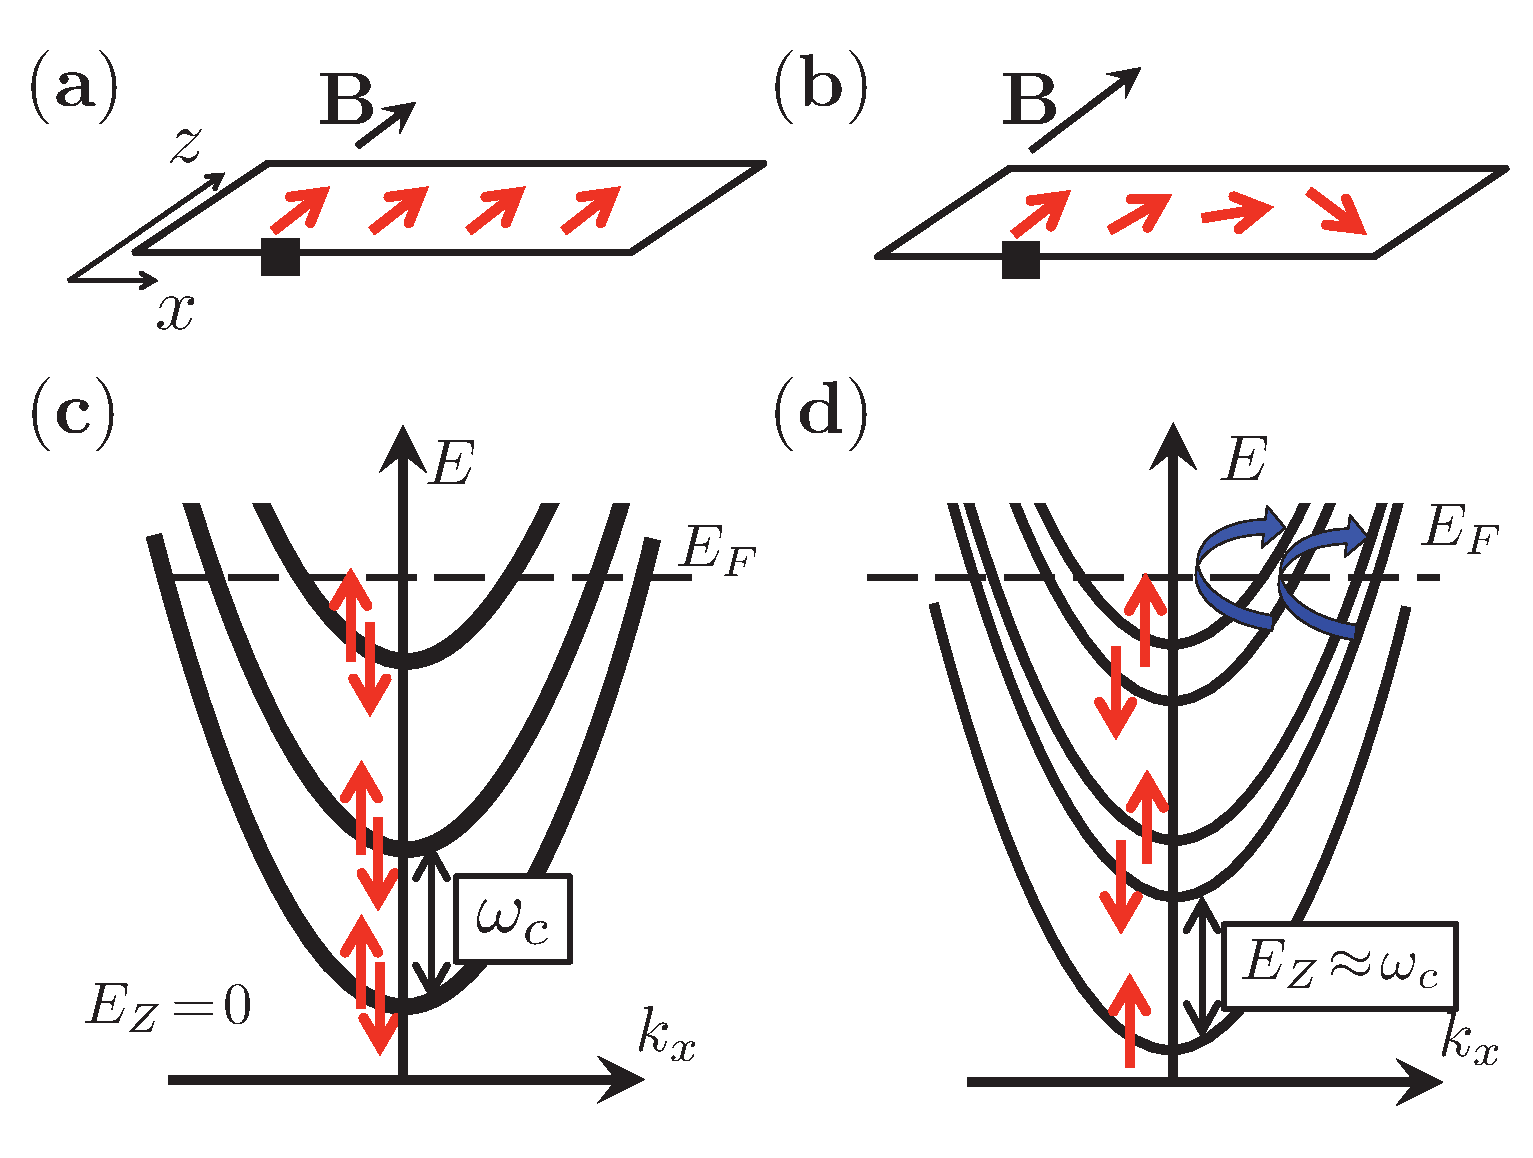
\includegraphics[width=1.0\columnwidth]{fig1.eps}
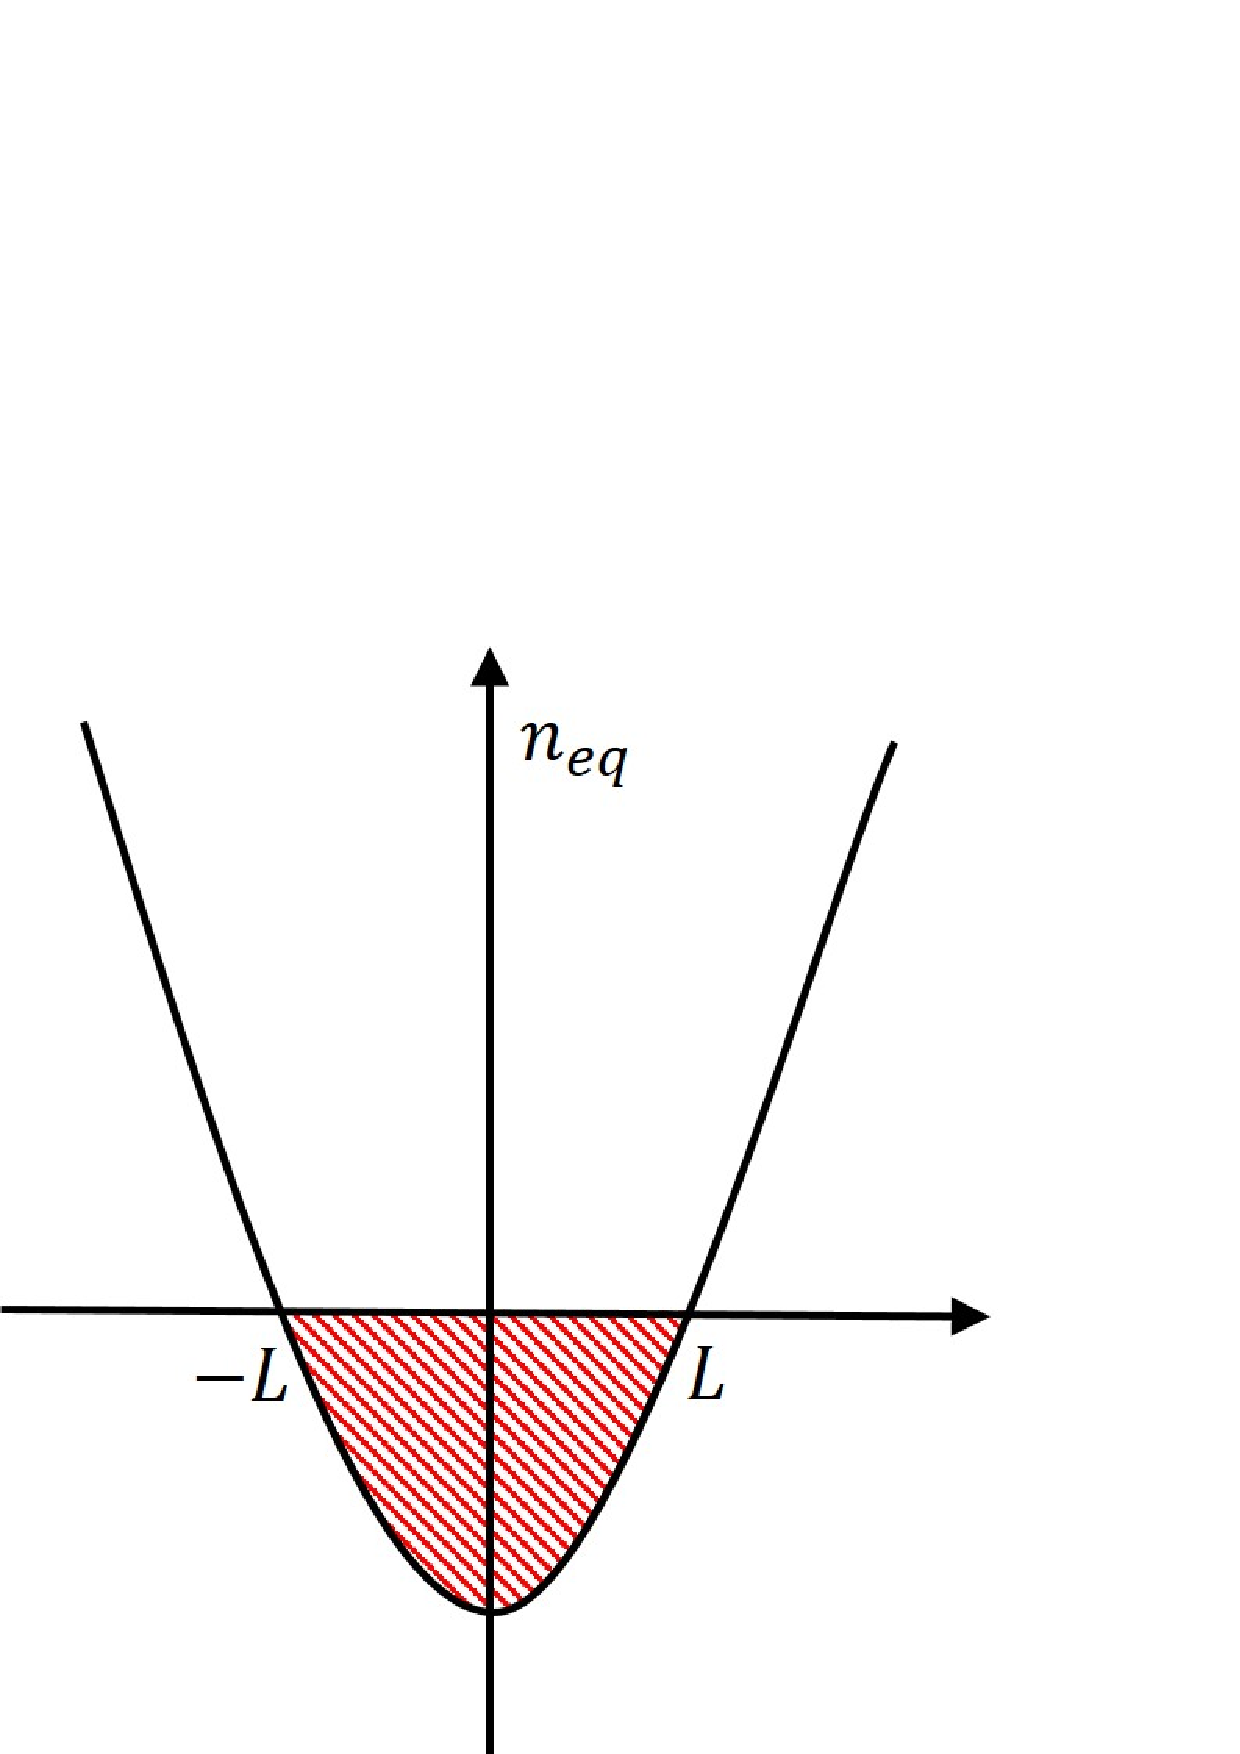
\includegraphics[height=0.5\columnwidth]{BC1.jpg}
\caption{The equilibrium density, $n_{eq}$ as a function of $\bm{z}$}
\label{fig:BC1}
\end{center}
\end{figure}

At equilibrium,
\be
\frac{kz^2}{2}+nV_0 \equiv \mathrm{const} = \frac{kL^2}{2}
\ee
where, L is the extent of the condensate, and
\be
n = n_0 \left(1-\left(\frac{z}{L}\right)^2\right)
\ee
where the parameter $n_0$ is given by
\be
n_0 = n(z=0) = \frac{kL^2}{2V_0}
\ee
These parameters set the conditions for the equilibrium density:
\be
m\frac{\partial^2 \delta n}{\partial t^2} = V_0 \bm{\nabla}\cdot \left(n_{eq} \bm{\nabla} \delta n \right)
\ee
or,
\be
\frac{m}{V_0} \frac{\partial^2 \delta n}{\partial t^2} = V_0 n_0 \partial_z \left(\left(1-\left(\frac{z}{L}\right)^2\right)\partial_z\delta n\right)
\ee
with the change of variable $z/L \equiv y$:
\be
\frac{L^2}{n_0} \frac{m}{V_0} \frac{\partial^2 \delta n}{\partial t^2} = \partial_y \left[\left(1-y^2\right)\partial_y \delta n\right]
\ee
But, we recognize that:
\be
\frac{L^2}{n_0} \frac{m}{V_0} = \frac{L^2m}{kL^2} \frac{2V_0}{V_0} = 2 \frac{m}{k} = \frac{2}{\omega_\perp^2}
\ee
Then we arrive at the following equation:
\be
\frac{\partial^2 \delta n}{\partial t^2} = \frac{\omega_\perp^2}{2} \partial_y \left[\left(1-y^2\right)\partial_y\delta n\right]
\ee
We  are particularly looking for solutions of the type $\delta n = \delta n_\omega e^{-i\omega t}$, which yields
\be
-\omega^2 \delta n_\omega = \frac{\omega_\perp^2}{2}\partial_y\left[\left(1-y^2\right)\partial_y\delta n\right]
\ee
We recognize this as the Legendre differential equation:
\be
\delta l^2 P_l = \frac{\omega_\perp^2}{2}\left[-l(l+1)P_l\right]
\ee
with
\be
\omega_l = \omega_\perp\sqrt{\frac{l(l+1)}{2}} \ , \ \delta n = P_l(y)e^{-i\omega t}
\ee
While $l=1$, $\delta n \propto n_0 y e^{-i\omega t}$. The time dependence of the velocity is given by:
\be
m\frac{\partial \bm{v}}{\partial t} = -V_0 \bm{\nabla}\delta n \Rightarrow -i\omega mv = -V_0n_0
\ee
So, the velocity $(\bm{v}(z)=\bm{v})$ is constant in space which is the Kohn mode of the condensate.

\section{Thermal Cloud in Pancake Geometry}
For the thermal cloud, we start by writing the continuity equation and the linearized Euler equation \cite{Pethic},
\bea
\frac{\partial \rho}{\partial t} + \bm{\nabla}\cdot(\rho \bm{v}) = 0 \\
\rho_{eq}\frac{\partial \bm{v}}{\partial t} = -\bm{\nabla}P + \rho\bm{f}
\eea
where, $\bm{f}$ is the force per unit mass: $\bm{f}=-\frac{1}{m}\bm{\nabla}V$, and at equilibrium, $\bm{\nabla}P_{eq}=\rho_{eq}\bm{f}$. Also, taking a time derivative of the previous equation:
\be\label{BCA*}
\rho_{eq} \frac{\partial^2 \bm{v}}{\partial t^2} = -\bm{\nabla} \left(\frac{\partial P}{\partial t}\right) + \frac{\partial \rho}{\partial t} \bm{f}
\ee
We specify the adiabatic conditions for ideal gas: $P/\rho^{5/3}=\textrm{const}$.
\subsection{The Case of a Monoatomic Classical Gas}
Here we will investigate the Kohn theorem for the pancake geometry in case of a classical monoatomic gas. We start by rewriting the adiabatic condition for ideal gas in the following form:
\be
\frac{dP}{P} + \frac{5}{3} \frac{d\mathcal{V}}{\mathcal{V}} = 0 
\ee
We know, for classical gas, $P\mathcal{V} = NkT$ and $E=\frac{3}{2} NkT$. With help of these relations, we find:
\be
dP = -\frac{NkT}{\mathcal{V}^2}d\mathcal{V} + \frac{NkdT}{\mathcal{V}} \ ; \ dE = \frac{3}{2}NkdT = -Pd\mathcal{V} (\mathrm{adiabatic \ compression})
\ee
and finally,
\be
dP=-\frac{P}{\mathcal{V}}d\mathcal{V}-\frac{2}{3}\frac{P}{\mathcal{V}}d\mathcal{V}=-\frac{5}{3}\frac{P}{\mathcal{V}}d\mathcal{V}
\ee
Now, we let $\bm{\xi}=\bm{v}dt$ be the displacement of the mass parcel of a fluid during time dt. As $P/\rho^{5/3}=\textrm{const}$, we have
\be
\frac{P(\bm{r}+\bm{\xi})}{\rho(\bm{r}+\bm{\xi})^{5/3}}=\frac{P_{eq}(\bm{r})}{\rho_{eq}^{5/3}(\bm{r})}
\ee
which yields,
\begin{align}
P(\bm{r})-P_{eq}(\bm{r}) &= \left(P_{eq}(\bm{r})-\bm{\xi}\frac{\partial P}{\partial \bm{r}}\right) \left[\frac{\rho_{eq}(\bm{r})+\delta\rho}{\rho_{eq}(\bm{r})-\bm{\xi}.\bm{\nabla}\rho_{eq}}\right]^{5/3}-P_{eq} \\
&= -\bm{\xi}\cdot\bm{\nabla}P_{eq}+\frac{5}{3}\frac{P_{eq}}{\rho_{eq}}\left(\delta \rho+\bm{\xi}\cdot\bm{\nabla}\rho_{eq}\right)
\end{align}
With $\bm{v}=\dot{\bm{\xi}}$:
\be\label{BCA1}
\frac{\partial P}{\partial t} = \frac{5}{3} \frac{P_eq}{\rho_eq}\left(\partial \delta \rho{\partial t} + \bm{v}\cdot\bm{\nabla}\rho_{eq}\right) - \bm{v}\cdot\bm{\nabla} P_{eq}
\ee
The continuity equation gives:
\be
\frac{\partial \delta \rho}{\partial t} + \bm{v}\cdot\bm{\nabla}\rho_{eq}+\rho_{eq}\bm{\nabla}\cdot\bm{v}=0
\ee
Then equation \eqref{BCA1} becomes:
\begin{align}
\frac{\partial P}{\partial t} &= -\frac{5}{3}P_{eq}\bm{\nabla}\cdot\bm{v}-\bm{v}\cdot\bm{\nabla}P_{eq} \\
&= -\frac{5}{3}P_{eq}\bm{\nabla}\cdot\bm{v}-\rho_{eq}\bm{f}\cdot\bm{v}
\end{align}
Thus,
\be\label{BCA**}
\frac{\partial P}{\partial t} = -\frac{5}{3}P_{eq}\bm{\nabla}\cdot\bm{v}-\rho_{eq}\bm{f}\cdot\bm{v}
\ee
At equilibrium, $P_{eq}=P_{eq}(\rho_{eq}.T)$.
\be
\bm{\nabla}P_{eq}=\frac{\partial P_{eq}}{\partial \rho_{eq}}\bm{\nabla}\rho_{eq}=\rho_{eq}\bm{f}
\ee
which means $\bm{\nabla}\rho_{eq}\parallel\bm{f}$
\be
(\bm{f}\cdot\bm{v})\bm{\nabla}\rho_{eq}=\bm{f}(\bm{v}\cdot\bm{\nabla})\rho_{eq}
\ee
Using equations \eqref{BCA*} and \eqref{BCA**}, we get:
\be
\frac{\partial^2 \bm{v}}{\partial t^2} = \frac{5}{3}\frac{P_{eq}}{\rho_{eq}}\bm{\nabla}(\bm{\nabla}\cdot\bm{v})+\bm{\nabla}(\bm{f}\cdot\bm{v})+\frac{2}{3}(\bm{\nabla}\cdot\bm{v})\bm{f}
\ee

For classical Gas, $\frac{p_{eq}}{\rho_{eq}}=\frac{kT}{m}$. Also, $\bm{v}(t)=\bm{v}e^{-i\omega t}$, $\bm{v}=(0,0,v)$, and for pancake geometry, $\bm{f}=-\omega_\perp^2z\hat{\bm{z}}$. Applying these conditions,
\be
-\omega^2v = \frac{5}{3} \frac{kT}{m} \partial_z^2v - \partial_z(\omega_\perp^2zv) - \frac{2}{3}\omega_\perp^2z\partial_zv
\ee
With the change of variables $z=y\sqrt{2kT/m\omega_\perp^2}$,
\be
\frac{6}{5\omega_\perp^2}(-\omega^2+\omega_\perp^2)v = \partial_y^2v - 2y\partial_yv
\ee
Which has the solution in the form of Hermite polynomial $v_n(y)-v_0H_n(y)$. $H_n(y)$ satisfies $y''-2xy'+2ny=0$. Thus, we have
\bea
\frac{6}{5\omega_\perp^2}(-\omega^2+\omega_\perp^2)H=-2nH_n \\
\omega=\omega_\perp\left(\frac{3+5n}{3}\right)^{1/2}
\eea
For $n=0$, $v_{n=0}=H_0(y)\equiv const$, $\omega=\omega_\perp\left(\frac{3+5\times 0}{3}\right)^{1/2}=\omega_\perp$. This is the Kohn theorem for the thermal cloud.
%\newpage

%%%%%%%%%%%%%%%%%%%%%%%%%%%%%%%%%%%%%%%%%%%%%
\section{The Coupled System}
%\label{app:tabfig:tables}
Here, we wish to investigate the behavior of the Bose condensate coupled with its thermal cloud confined inside the pancake geometry. To achieve this, first we need to write the complete sets of coupled equations for each of the two. Firstly, the complete Equations for Condensate are \cite{zaremba1998},
\bea 
\frac{\partial n_c}{\partial t} = - \bm{\nabla}\cdot \left(n_c \bm{v}_c\right) \\
m\left( \frac{\partial\bm{v}_c}{\partial t} + \frac{1}{2} \bm{\nabla}v^2_c \right) = - \bm{\nabla}\phi 
\eea
where,
\bea 
\bm{v}_c(\bm{r},t) \equiv \frac{\hbar}{m} \bm{\nabla} \theta (\bm{r},t) \\
\phi (\bm{r},t) \equiv \frac{1}{|\Phi(\bm{r},t)|} \hat{H}(\bm{r},t) |\Phi(\bm{r},t)| \\
\hat{H}(\bm{r},t) = - \frac{\hbar^2 \bm{\nabla}^2}{2m} + U (\bm{r}) + 2g\tilde{n}(\bm{r},t) + gn_c(\bm{r},t) \\
\Phi(\bm{r},t)=|\Phi(\bm{r},t)|e^{i\theta(\bm{r},t)} \\
n_c(\bm{r},t) = |\Phi(\bm({r},t)|^2 \\
g = 4\pi a \hbar^2/m
\eea

And now, the complete equations for thermal cloud are,
\bea
\frac{\partial\tilde{n}}{\partial t} + \bm{\nabla}\cdot(\tilde{n}\bm{v}_n) = 0 \\
m\tilde{n} \left( \frac{\partial\bm{v}_n}{\partial t} + (\bm{v}_n\cdot\bm{\nabla})\bm{v}_n \right) = -\bm{\nabla}\tilde{P} - \tilde{n}\bm{\nabla}U \\
\frac{\partial\tilde{\epsilon}}{\partial t} + \frac{5}{3} \ \bm{\nabla} \cdot (\tilde{\epsilon}\bm{v}_n) = \bm{v}_n \cdot \bm{\nabla}\tilde{P}
\eea

where,
\be \tilde{n}(\bm{r},t) \equiv \int \frac{d^3p}{h^3} f_0(\bm{r},\bm{p},t) = \frac{1}{\Lambda^3} g^{3/2}(z(\bm{r},t)) \ee
with,
\bea
z(\bm{r},t) \equiv e^{\beta(\bm{r},t)\left[\mu(\bm{r},t)-U(\bm{r},t)\right]} \\
\Lambda(\bm{r},t) = 2\pi\hbar^2/mk_BT(\bm{r},t)^{1/2} \\
f_0(\bm{r},\bm{p},t) = \left[exp\left[\beta\{\frac{1}{2m}\left[\bm{p}-m\bm{v}_n\right]^2+U-\mu\}\right]-1\right]^{-1} 
\eea

$\tilde{\epsilon}$ is the non-convective part of kinetic energy density
\bea
\tilde{P} = \frac{2}{3}\tilde{\epsilon} \\
\bm{\nabla}\tilde{P}=-\tilde{n}_0\bm{\nabla}U_0
\eea
where,
\be U_0 = U + 2g\tilde{n}_0 + 2gn_{c0} \ee
The eigenvalue equation for the Hamiltonian operator is,
\be \label{BCBA}
H\Phi=\left(U+2g\tilde{n}+gn_c\right)\Phi
\ee
We define $\phi$ as,
\be
\phi \equiv \frac{1}{|\Phi|} H|\Phi| = U + 2g\tilde{n}+gn_c
\ee
or,
\be
\delta \phi = 2g\delta\tilde{n}+g\delta n_c
\ee

Next, we linearize both of the system of equations. For the condensate, we have
\be\label{BCB1a}
\frac{\partial\delta n_c}{\partial t} = -\bm{\nabla} \cdot (n_{c0}\delta\bm{v}_c)
\ee
\be\label{BCB1b}
m \frac{\partial\delta\bm{v}_c}{\partial t} = -\bm{\nabla}\delta\phi 
\ee

and for thermal cloud,
\be\label{BCB2a}
\frac{\partial\delta\tilde{n}}{\partial t} = -\bm{\nabla}.(\tilde{n}_0\delta\bm{v}_n)
\ee
\be\label{BCB2b}
m\tilde{n}_0\frac{\partial\delta\bm{v}_n}{\delta t} = -\bm{\nabla}\delta\tilde{P}-\delta\tilde{n}\bm{\nabla}U_0-2g\tilde{n}_0\bm{\nabla}(\delta\tilde{n}+\delta n_c)
\ee
\be\label{BCB2c}
\frac{\partial \delta\tilde{P}}{\partial t} = - \frac{5}{3} \ \bm{\nabla} \cdot (\tilde{P}_0\delta\bm{v}_n)+\frac{2}{3} \ \delta\bm{v}_n \cdot \bm{\nabla}\tilde{P}_0
\ee

\subsection{Verification of Kohn Mode}
To verify the Kohn theorem, we consider the small displacement of kind
\be\label{BCB3}
\bm{\eta}(t) = \bm{\eta}_0 cos\omega_it
\ee
The confinement potential is of the shape
\be\label{BCB4}
U = \frac{1}{2} \ m(\omega_x^2x^2+\omega_y^2y^2+\omega_z^2z^2)
\ee
Therefore,
\be\label{BCB5}
\delta\tilde{n}=-\bm{\nabla}\tilde{n}_0 \cdot \bm{\eta}(t) \ \ \ \delta n_c = -\bm{\nabla}n_{c0} \cdot \bm{\eta}(t)
\ee
and,
\be\label{BCB6}
\delta\bm{v}_c = \delta\bm{v}_n = \dot{\bm{\eta}}(t)
\ee
It is important to note that the above equation \eqref{BCB6} is spatially independent. Now, there are three possible choices for $\bm{\eta}$, namely, $\eta \hat{\bm{x}}$, $\eta \hat{\bm{y}}$ and $\eta \hat{\bm{z}}$. We choose to take $\bm{\eta}=\eta \hat{\bm{z}}$ for definiteness.

First observe that equation \eqref{BCB1a} is valid. With use of \eqref{BCB5}, we can rewrite it as:
\be 
 \frac{\partial}{\partial t} \left(-\bm{\nabla}n_{c0} \cdot \bm{\eta} \right) = -\bm{\nabla} \cdot \left(n_{c0} \dot{\bm{\eta}}\right) \ee
which is valid because $n_{c0}$ is independent of $t$ and $\bm{\eta}$ is independent of space.

Now, equation \eqref{BCB1b}:
\be m \frac{\partial\delta\bm{v}_c}{\partial t} = -\bm{\nabla}\delta\phi \ee
from \eqref{BCBA} and \eqref{BCB6}:
\be\label{BCB7}
m \frac{\partial}{\partial t} \dot{\bm{\eta}}(t) = -\bm{\nabla}(2g\delta\tilde{n}+g\delta n_c)
\ee
using \eqref{BCB5}:
\bea
m \frac{\partial}{\partial t} \dot{\bm{\eta}}=-g\bm{\nabla} \cdot (-2\bm{\nabla}\tilde{n}_0 \cdot \bm{\eta}(t)-\bm{\nabla}n_{c0} \cdot \bm{\eta}(t)) \\
m \frac{\partial}{\partial t} \dot{\bm{\eta}} = g\bm{\nabla}(\bm{\nabla}(2\tilde{n}_0+n_{c0}) \cdot \bm{\eta})
\eea
with $\bm{\eta}=\eta \hat{\bm{z}}$,
\be
-m\omega_z^2\cos{(\omega_zt)}\eta_0\hat{\bm{z}}=g\bm{\nabla}\cdot(\partial_z(2\tilde{n}_0+n_{c0})\eta_0\cos{(\omega_zt)})
\ee
or,
\be
\partial_z^2(g(2\tilde{n}_0+n_{c0})+\frac{1}{2} \ m\omega_z^2z^2)=0
\ee
which is correct because $(\frac{1}{2} \ m\omega_z^2z^2+2g\tilde{n}_0+gn_{c0})$ is constant in $(x,y,z)$. \\
Now, we will verify equations \eqref{BCB1a} through \eqref{BCB2c}. First, from equation \eqref{BCB2a},
\bea
\frac{\partial\delta\tilde{n}}{\partial t} = -\bm{\nabla}\cdot(\tilde{n}_0\delta\tilde{v}_n) \\
\mathrm{or,} \frac{\partial}{\partial t}(-\bm{\nabla}\tilde{n}_0\cdot\bm{\eta})=-\bm{\nabla}\cdot(\tilde{n}_0\frac{\partial}{\partial t}\bm{\eta})
\eea
which is evidently a valid relation. Now, from equation \eqref{BCB2c}, we have
\begin{align}
\frac{\partial\delta\tilde{P}}{\partial t} &= - \frac{5}{3} \ \bm{\nabla}.(\tilde{P}_0\delta\bm{v}_n)+\frac{2}{3} \ \delta\bm{v}_n\cdot\bm{\nabla}\tilde{p}_0 \\
&= -\frac{5}{3} \ (\bm{\nabla}\tilde{P}_0)\cdot\dot{\bm{\eta}}+\frac{2}{3} \ (\bm{\nabla}\tilde{P}_0)\cdot\dot{\bm{\eta}} \\
&= - (\bm{\nabla}\tilde{P}_0)\cdot\dot{\bm{\eta}}
\end{align}

which gives us,
\be\label{BCB8}
\delta\tilde{P} = -(\bm{\nabla}\tilde{P}_0)\cdot\bm{\eta}
\ee

Equation \eqref{BCB2b}, with help of \eqref{BCB8} can be rewritten as
\be
m\tilde{n}_0 \frac{\partial}{\partial t}\dot{\bm{\eta}} = -\bm{\nabla}\left[(-\bm{\nabla}\tilde{P}_0)\cdot\bm{\eta}\right] - \left[(-\bm{\nabla}\tilde{n}_0)\cdot\bm{\eta}\right]\bm{\nabla}U_0-2g\tilde{n}_0(\bm{\nabla}\delta\tilde{n}+\bm{\nabla}\delta n_c)
\ee
using equation \eqref{BCB7} with $\bm{\eta}=\eta\hat{\bm{z}}$ (considering z-components only),
\be
-\tilde{n}_0\partial_z(2g\delta\tilde{n}+g\delta n_c) = (\partial_z^2\tilde{P}_0)\eta+(\partial_z\tilde{n}_0)(\partial_zU_0)\eta-2g\tilde{n}_0\partial_z(\delta\tilde{n}+\delta n_c)
\ee
or,
\be\label{BCB9}
\partial_z^2\tilde{P}_0\eta+(\partial_z\tilde{n}_0)(\partial_zU_0)\eta-g\tilde{n}_0\partial_z\delta n_c =0
\ee
but, we know, $\bm{\nabla}\tilde{P}_0=-\tilde{n}_0\bm{\nabla}U_0$. Then \eqref{BCB9} reduces to
\be
-\partial_z^2\left[U+2g\tilde{n}_0+gn_{c0}\right]=0
\ee
which is correct because $U+2g\tilde{n}_0+gn_{c0}$ is constant in $z$.
%AI
This proves that the collective oscillations in our confined condensate-thermal cloud system are protected from interactions and the Kohn theorem holds for such systems.

\section{Anharmonicity in the Condensate}
%AI
Here we will investigate the effects of potential anharmonicity in the condensate. We start with the linearized equations as before:
\be\label{BCC1}
\frac{m}{U_0} \frac{\partial^2\delta n}{\partial t^2} = U_0 \bm{\nabla} (n_{eq}\bm{\nabla}\delta n)
\ee
Now we introduce a small non-parabolicity controlled by the parameter $\varepsilon$:
\bea\label{BCC2}
n_{eq} = \frac{1}{U_0} \frac{k(L^2-z^2)}{2} + \varepsilon\frac{(z^4-L^4)}{4} \\
= n_0 \left(1-\left(\frac{z}{L}\right)^2\right) + n_1\left(\left(\frac{z}{L}\right)^4-1\right)
\eea

where, $n_0 \equiv \frac{kL^2}{2U_0}$ \& $n_1 \equiv \frac{\varepsilon L^4}{4}$ \\
from equation \eqref{BCC1}:
\be
\frac{\partial^2\delta n}{\partial t^2} = \frac{U_0}{m} \frac{\partial}{\partial z} \left[\left[n_0\left(1-\left(\frac{z}{L}\right)^2\right) + n_1\left(\left(\frac{z}{L}\right)^4-1\right)\right]\frac{\partial}{\partial z}\delta n\right]
\ee
now, we consider $\delta n \propto e^{-i\omega t}$ and a change of variable $\frac{x}{L} = y$
\be
-\omega^2\delta n = \frac{n_0U_0}{mL^2} \frac{\partial}{\partial y} \left[\left[\left(1-y^2\right)+\frac{n_1}{n_0}\left(y^4-1\right)\right]\frac{\partial}{\partial y} \delta n\right]
\ee
with $\frac{\omega_\perp^2}{2}$:
\be
-\omega^2\delta n = \frac{\omega_\perp^2}{2} \frac{\partial}{\partial y} \left[\left(1-y^2\right)\frac{\partial}{\partial y}\delta n\right] + \frac{\omega_\perp^2}{2} \frac{n_1}{n_0} \frac{\partial}{\partial y} \left[\left(y^4-1\right)\frac{\partial}{\partial y}\delta n\right]
\ee
with $\lambda\equiv\omega^2$, we arrive at the eigenvalue equation, which is just the Legendre differential equation:
\bea
\lambda\delta n = -\frac{\omega_\perp^2}{2} \ \frac{\partial}{\partial y}\left[\left(1-y^2\right)\frac{\partial}{\partial y}\right]\partial n \\
\lambda = l(l+1), l=0,1,2,3,... \\
\delta n_l(y)=P_l(y)\sqrt{\frac{2l+1}{2}}
\eea
\\
so far we have:
\be
\lambda\delta n = H_0 + H_1
\ee
where, $H_0\equiv-\frac{\omega_\perp^2}{2} \frac{\partial}{\partial y} \left[\left(1-y^2\right)\frac{\partial}{\partial y}\delta n\right]$ and $H_1\equiv-\frac{\omega_\perp^2}{2}\frac{n_1}{n_0}\frac{\partial}{\partial y}\left[\left(y^4-1\right)\frac{\partial}{\partial y}\delta n\right]$ \\
with, $\lambda_l^0 = l(l+1)$ and $\delta n_l^0 = \sqrt{\frac{2l+1}{2}} \ P_l(y)\equiv f_l^0$. Now, we want to find the first order correction to the eigenvalue: $\lambda_l^1$.
\bea
\lambda_l^1=\left<f_l^0|H_1|f_l^0\right> \\
= - \left(\frac{2l+1}{2}\right) \frac{\omega_\perp^2}{2} \frac{n_1}{n_0} \int_{-1}^{1}P_l(y)\frac{\partial}{\partial y}\left[\left(y^4-1\right)\frac{\partial}{\partial y}P_l(y)\right]dy \\
\Rightarrow \lambda_1^1 = -\left(\frac{\omega_\perp^2}{2} \frac{n_1}{n_0}\right)\left(\frac{12}{5}\right)
\eea

\section{Anharmonicity in the Thermal Cloud}
We start with the usual equations:
\be\label{BCD1}
\frac{6}{5} \frac{1}{\omega_\perp^2} (-\omega^2+\omega_\perp^2)v=\partial_y^2v-2y\partial_yv
\ee
\be\label{BCD2}
\frac{\partial^2\bm{v}}{\partial t^2} = \frac{5}{3} \frac{P_{eq}}{\rho_{eq}}\bm{\nabla}(\bm{\nabla}\cdot\bm{v})+\bm{\nabla}(\bm{f}\cdot\bm{v})+\frac{2}{3}(\bm{\nabla}\cdot\bm{v})\bm{f}
\ee
For classical gas, $\frac{P_{eq}}{\rho_{eq}} = \frac{kT}{m}$. We also consider $v\propto e^{-i\omega t}\bm{x}$. Under These considerations, $\bm{f}$ takes the form:
\be
\begin{split}
\bm{f} & = -\bm{\nabla}U = -\frac{\partial}{\partial z} \left[\frac{1}{2} \omega_\perp^2 z^2 + \frac{\varepsilon}{4m}\left(z^4-L^4\right)\right]\hat{\bm{z}} \\
& = \left(-\omega_\perp^2z - \frac{\varepsilon}{m}z^3\right)\bm{z} \\
& \equiv (f_0 + f_1)\bm{z}
\end{split}
\ee
Then \eqref{BCD2} becomes:
\be\label{BCD3}
-\omega^2v=\frac{5}{3} \frac{kT}{m} \frac{\partial^2v}{\partial z^2}-\frac{\partial}{\partial z} \left(\omega_\perp^2zv+\frac{\varepsilon}{m}z^3\frac{\partial v_z}{\partial z}\right)
\ee
or,
\be
\left(-\omega^2+\omega_\perp^2\right)v=\frac{5}{3}\frac{kT}{m}\frac{\partial^2v}{\partial z^2}-\frac{5}{3}\omega_\perp^2z\frac{\partial v}{\partial z}-\frac{3\varepsilon}{m}z^2v-\frac{5}{3}\frac{\varepsilon}{m}z^3\frac{\partial v}{\partial z}
\ee
Performing a change of variable: $x\equiv y\sqrt{2kT/m\omega_\perp^2}$ and substituting $\eta\equiv\left(\frac{m\omega_\perp^2}{2kT}\right)^\frac{1}{2}$, we arrive at the following equation:
\be
\frac{6}{5} \left(\frac{-\omega^2+\omega_\perp^2}{\omega_\perp^2}\right)v=\frac{\partial^2 v}{\partial y^2} - 2y\frac{\partial v}{\partial y} - \frac{18\varepsilon}{5\eta^2m}y^2v-\frac{2\varepsilon}{\eta^2m}y^3\frac{\partial v}{\partial y}
\ee
we define:
\begin{align}
\lambda &\equiv \frac{6}{5} \left(\frac{-\omega^2+\omega_\perp^2}{\omega_\perp^2}\right) \\
H_0 &\equiv \frac{\partial^2 v}{\partial y^2} - 2y\frac{\partial v}{\partial y} \\
H_1 &\equiv - \frac{18\varepsilon}{5\eta^2m}y^2v-\frac{2\varepsilon}{\eta^2m}y^3\frac{\partial v}{\partial y}
\end{align}


Then the equation $H_0v=\lambda v$ is the Hermite polynomial equation. Thus,
\begin{align}
&\frac{6}{5}\left(\frac{-{\omega_n^0}^2+\omega_\perp^2}{\omega_\perp^2}\right) = -2n \\
\Rightarrow \ \ &{\omega_n^0}^2 = \left(1+\frac{5}{3}n\right)\omega_\perp^2 \\
&\lambda_n^0 \equiv \frac{6}{5}\left(\frac{-{\omega_n^0}^2+\omega_\perp^2}{\omega_\perp^2}\right)
\end{align}

The first-order corrections to the eigenvalues are given by:
\begin{align}
\lambda_n^1 &= \left(\frac{1}{\sqrt{\pi}2^nn!}\right) \int_{-\infty}^\infty H_n\hat{H}_1H_ne^{-y^2}dy \\
\lambda_0^1 &= -\frac{9\varepsilon}{5\eta^2m}
\end{align}
%\section{Some Figures}
%\label{app:tabfig:figures}


\chapter{Conclusions}
\label{sec:Conclusions}

To conclude, we studied the effect of electron interaction on the collective and p-h excitations in a laterally confined two-dimensional Fermi gas.
The spectrum of confined electrons splits into subbands of transverse quantization.
We focused on the transversal excitations across the channel controlled by the subband separation energy scale.

When the Zeeman splitting is tuned to the subband separation a special type of  resonance, the BSR is detected in the dc transport measurements of Ref.~\cite{Frolov2009,Frolov2009a}.
Hence we analyzed the class of collective modes adiabatically connected to the spin flip intersubband p-h excitations which become soft at the BSR. 
The BSR measurements of \cite{Frolov2009} probe the individual p-h excitations.
We showed however relying on the perturbation theory that for a weak, short range interaction and sufficiently close to the BSR such p-h excitations are indistinguishable from the collective spin sloshing mode.
Therefore finding the frequency of the collective spin sloshing mode at the same time allows us to determine the shift of the BSR caused by interactions.

To meet this goal we applied the Fermi liquid theory to identify and analyze the spin sloshing mode.
It combines the features of two other more familiar collective excitations.
The first is the density oscillations across the channel, with amplitude vanishing at the center of the channel and is referred to as sloshing, or Kohn mode. 
The second is the collective spin precession mode in the presence of a Zeeman splitting.

The spin-sloshing mode is the collective spin precession with an amplitude growing linearly away from the center of the channel, see Fig.~\ref{fig:slosh}.
We demonstrated that the Kohn theorem does not apply to it, and found its frequency renormalization due to a weak and short range interaction.

Finally, by combining the above results we obtained the physical picture of interaction effect on the BSR.
We start by setting the Zeeman splitting to the subband separation in a Fermi gas.
Then the spin-flip intersubband p-h excitations have a zero energy, and the system is at resonance.
When a weak interaction is turned on these p-h excitations remain degenerate with their common energy becoming non-zero.
Hence, the interaction detunes the resonance.
To tune it back the Zeeman splitting must be accordingly adjusted.
It follows that the resonant magnetic field is modified by interactions. 
To quantify this statement we used the analytical expression for the energy of a spin sloshing mode was obtained within the Fermi liquid theory.

In our analysis we assumed the confining potential to be parabolic with the equidistantly separated subbands, see Eq.~\eqref{M17}.
Although the realistic confining potential is never strictly harmonic, the deviation from parabolic potential profile is in many cases small. 
If we take the non-parabolic part of the confining potential in the form,
$\delta V_{np}(z) = (\epsilon/4)z^4$ then the continuum of the p-h excitations is split due to the variation of the level shift $\delta E_{n\alpha}(k_x) \approx \langle n | \delta V_{np}| n \rangle $ with the subband index $n$.
The unharmonicity effect is negligible provided the energy shift due to the interactions, $\omega_c (V_{\rho} \! -\!  3 V_s)\nu$, Eq.~\eqref{result1_b} exceeds the typical value of $\delta E_{n\alpha}(k_x)$. 
This gives the upper bound, $\epsilon < (m \omega_c^2/ 2 E_F)^2 \omega_c m (V_{\rho} \! -\!  3 V_s)$, as we estimate $\langle z^4 \rangle \sim  (2 E_F/ m \omega_c^2)^2$.

In summary, the interaction induced shift of the BSR is obtained by tracing the frequency renormalization of the collective spin sloshing mode.
The shift of the BSR is a consequence of the non-existence of the Kohn theorem for this mode.

The hydrodynamic description requires short equilibration length $\ell$. Thus validity of our theory is limited by the condition $\ell\ll a$, which imposes certain restriction on temperature. Specifically, for the Fermi liquids $\ell=v_F\tau_{ee}$ is determined by collisions with the typical rate $\tau^{-1}_{ee}\sim T^2/E_F$. Since $\omega_\perp\sim v_F/a$, hydrodynamic regime is realized at temperatures $T>T_h$ above the crossover scale $T_h\sim\sqrt{\omega_\perp E_F}\sim E_F/\sqrt{N}$, where $N$ is the number of occupied sub-bands of the transversal quantization. It also follows that with necessity hydrodynamics requires $T\gg\omega_\perp$. While this inequality is reasonably satisfied for the cold gases that are confined by a very shallow potential, it obviously breaks in the ultra-cold limit where collisionless regime prevails. In the latter case attenuation coefficient of the Kohn mode is expected to follow quadratic temperature dependence $\tau^{-1}_{1}\propto \alpha T^2/E_F$ based on the Pauli principle and phase space restrictions argument, whereas in the hydrodynamic regime $\tau^{-1}_{1}\propto 1/T^2$ in accordance with Eq.~(\ref{tau-K}). The nonmonotonic temperature dependence of the decay rate has been observed experimentally~\cite{Riedl}.  

Our hydrodynamic approach has interesting parallels with the Luttinger liquid description of collective modes in confined inhomogeneous one-dimensional gases ~\cite{Citro}. The eigenvalue equation for the normal eigenmodes in that case, analogous to our Eq.~(\ref{normal-modes-eq}), is given by  
\begin{equation}\label{eigenmodes-LL}
-\omega^2_n\chi_n(z)=v(z)K(z)\partial_z\left(\frac{v(z)}{K(z)}\partial_z\chi_n(z)\right)
\end{equation}
where Luttinger liquid interaction parameter satisfies the relation\\ $v(z)K(z)=\pi \rho(z)/m^2$. This equation is supplemented by the boundary condition $\chi_n(\pm a)=0$ and normalization condition $\int^{a}_{-a} dz \chi_j(z)\chi_j(z)/v(z)K(z)=\delta_{ij}$. For the particular choice of $v(z)=v_0\sqrt{1-z^2/a^2}$ and $K(z)=K_0(1-x^2/a^2)^\gamma$ the solutions $\chi_n(z)$ are obtained in terms of Gegenbauer polynomials with the spectrum of excitations $\omega^2_n=(v_0/a)^2(n+1)(n+2\gamma+1)$~\cite{Citro,Petrov1,Stringari}. In the model of $\gamma=2$, the problem simplifies to the case of Legendre polynomials~\cite{Petrov2} with the spectrum of excitations analogous to our result (\ref{omega-n}). Another interesting limit is $\gamma=0$, which corresponds to the case of the Tonks-Girardeau gas, where the Gegenbauer polynomials reduce to Chebyshev polynomials. Inclusion of dissipative terms into Eq.~(\ref{eigenmodes-LL}) requires consideration of corrections to Luttinger liquid model which account for the inelastic scattering of bosons and ultimately describe equilibration processes. As recently shown such generalization is possible both in the limit of weak \cite{AL} and strong \cite{Matveev} interactions and application of this formalism to the problem of decay of collective modes is an interesting problem for future research. Along this rout one may hope to find a unified description, which interpolates between the quantum~\cite{Matveev} and classical~\cite{Andreev} hydrodynamic regimes of Luttinger liquids, and which is broadly applicable for arbitrarily strong interactions.  

In chapter 4, we established that for a confined Bose-Einstein condensate coupled with its thermal cloud in a pancake geometry, the collective modes are not affected by interactions and the Kohn theorem holds. However, for any departure of the confinement potential from parabolicity, the collective modes are shifted in frequency.


% app0.tex (silly little file to separate chapters from appendices)
\appendix
\titleformat{\chapter}[display]   
{\normalfont\large\bfseries\centering}{\chaptertitlename\ \thechapter}{10pt}{\large}   
\titlespacing*{\chapter}{0pt}{-20pt}{25pt}
%\setcounter{secnumdepth}{1}
%\setcounter{section}{0}

\chapter{Hydrodynamics of Homogeneous Liquids}
\section{Energy Conservation Equation for the Isentropic Flow in the Potential Field}%MK, Eq.~\eqref{s_cons}.}
\label{app:s_cons}
\setcounter{equation}{0}

It is often useful to express the entropy conservation condition, \eqref{s_cons} in a form of equations satisfied by the energy per unit mass, $\epsilon$.
Note that in the presence of the external potential, $U$, the energy  $\epsilon$ includes neither the kinetic energy of the macroscopic energy of the flow nor  the potential energy in the external field.
The latter, therefore has to be included in the energy conservation equation explicitly.
Consider the element of a fluid containing the fixed amount of particles, $N$ of mass $m$ at times $t$ and $t + d t$.
Let the energy, entropy and volume change during the  considered time interval be denoted as $dE$, $dS$ and $dV$.
Then the general thermodynamic formula
\be\label{dE}
d E = T d S - p d V + \mu d N
\ee
gives for the change in the course of the isentropic  flow of a fixed mass of a fluid,
\be
D \epsilon = - p \frac{d V}{ N m}  = - \frac{ p}{\rho} \frac{ d V }{ V} 
\ee
which expresses the change in the energy per unit mass in terms of the fractional volume increment, $d V / V$.
The fractional volume increment is due to the finite divergence of the flow velocity,
\be
\frac{ d V }{d t V} = \bm{\nabla} \cdot \bm{v} \, .
\ee
And we finally obtain Eq.~\eqref{alt_s_cons1}, which thanks to
%As a result thanks to 
the continuity Eq.~\eqref{cont} under the conditions of the isentropic flow, \eqref{s_cons}, the energy density per unit mass,  satisfies the following equation,  
\be\label{alt_s_cons2}
 \frac{\partial \rho \epsilon}{\partial t } + \bm{\nabla} (\bm{v} \rho \epsilon)= -  p \bm{\nabla} \cdot \bm{v} \, ,
\ee
where $\rho \epsilon$ is the energy per unit volume.

We now demonstrate that Eq.~\eqref{alt_s_cons1} is equivalent to the energy conservation expressed in the form, Eq.~\eqref{e_cons}.
First we write it as
\be\label{alt_s_cons3}
 \frac{\partial \rho (\epsilon + v^2/2 +U/m)}{\partial t } 
 -\frac{\partial \rho (v^2/2)}{\partial t } 
 -(U/m)\frac{\partial \rho }{\partial t }
  + \bm{\nabla} [\bm{v} (\rho \epsilon + p)] - \bm{\nabla} p \cdot  \bm{v} =0 \, ,
\ee
where we have used the fact that the potential energy $U(\bm{r})$ is time independent.
The condition that is required for the energy conservation to hold. 
Now write, using the continuity equation, \eqref{cont} 
\be\label{alt_s_cons4}
\frac{\partial \rho (v^2/2)}{\partial t } =
- \bm{\nabla}\cdot ( \rho \bm{v} ) v^2/2 + \rho \partial_t v^2/2
\ee
We further have,
\be\label{alt_s_cons5}
\frac{\partial \rho (v^2/2)}{\partial t } =
- \bm{\nabla}\cdot ( \rho \bm{v}  v^2/2 ) +    \rho \bm{v} \cdot \bm{\nabla}(v^2/2 )+ \rho \bm{v} \cdot \partial_t \bm{v}
\ee
In addition we write using the continuity equation, \eqref{cont} again,
\be\label{alt_s_cons5a}
(U/m)\frac{\partial \rho }{\partial t } =- (U/m) \bm{\nabla} \cdot (\rho \bm{v} ) = -\bm{\nabla} \cdot [ (U/m) \rho \bm{v} ] + \rho \bm{v} \cdot \bm{\nabla}  ( U/m).
\ee
Substitution of Eqs.~\eqref{alt_s_cons5} and \eqref{alt_s_cons5a} to Eq.~\eqref{alt_s_cons3} gives
\begin{align}\label{alt_s_cons6}
 \frac{\partial \rho (\epsilon + U/m + v^2/2)}{\partial t } &
 + \bm{\nabla}\cdot [ \rho \bm{v} (\epsilon + U/m+ p/\rho + v^2/2 ) ] 
 \notag \\
& -   \rho \bm{v} \cdot 
 [ 
 \bm{\nabla} \cdot v^2/2 + \partial_t \bm{v}
+ (\bm{\nabla} p)/\rho + \bm{\nabla} U/m] =0 \, .
\end{align}
Since 
\be\label{vi}
 \bm{\nabla} \cdot v^2/2 = \bm{v} \times [\bm{\nabla} \times \bm{v}] + (\bm{v} \cdot \bm{\nabla }) \bm{v}
\ee
we have according to the Euler equation, \eqref{Euler1}
\begin{align}\label{alt_s_cons7}
& \bm{v} \cdot 
 [ 
 \bm{\nabla} \cdot v^2/2 + \partial_t \bm{v}
+ \bm{\nabla} p/\rho+ \bm{\nabla} U/m] 
\notag \\
& =
\bm{v} \cdot 
 [ 
 (\bm{v} \cdot \bm{\nabla }) \bm{v} + \partial_t \bm{v}
+ \bm{\nabla} p/\rho + \bm{\nabla} U/m] = 0
\end{align}
Finally, substitution of Eq.~\eqref{alt_s_cons7} in Eq.~\eqref{alt_s_cons6} yields energy conservation Eq.~\eqref{e_cons}.

\section{Thermodynamic Identities}
\label{app:FL_s}



The identity, 
\begin{align}\label{sound13}
\left(\frac{\partial P}{\partial \rho} \right)_{s} =\frac{n}{m} \left(\frac{\partial \mu}{\partial n} \right)_{s}
\end{align}

\noindent
{\it Proof:}
%Here we demonstrate the equivalence of \eqref{FL19} and the relation \eqref{s_13}.
From the thermodynamic relation \eqref{dE} we have the Maxwell relation 
\be\label{MR1}
- \left(\frac{\partial P}{\partial N} \right)_{S,V} = \left(\frac{\partial \mu}{\partial V} \right)_{S,N}\, .
\ee
As a result,
 \be\label{MR2}
\frac{V}{m} \left(\frac{\partial P}{\partial N} \right)_{S,V} = \left(\frac{\partial P}{\partial \rho} \right)_{s}\, ,\quad
\frac{V}{m} \left(\frac{\partial \mu}{\partial V} \right)_{S,N} = -\frac{N}{m} \left(\frac{\partial \mu}{\partial N} \right)_{S,V}=
 -\frac{n}{m} \left(\frac{\partial \mu}{\partial n} \right)_{s}
\ee
Equations \eqref{MR1} and \eqref{MR2} yield Eq.~\eqref{sound13}.
%MK NEW SECTION


%\section{Relation Between the Adiabatic and Isothermal Susceptibilities}
%\label{app:ratio}

Identity, Eq.~\eqref{rat},
\begin{align*}
\frac{(\partial p / \partial \rho)_s }{(\partial p / \partial \rho)_T } = \frac{c_p}{c_V}\, .
\end{align*}

%In this appendix we prove the relation \eqref{rat}.

\noindent{\it Proof:}
Let us denote the Jacobian, $J$ of transformation from the variables $(x,y)$ to the variables $(u,v)$ by 
\be
J = \frac{\partial(u,v)}{\partial(x,y)}.
\ee
Then,
\be
\frac{ \partial (p, s) }{ \partial (\rho, s)} = \frac{ \partial (p, s) }{ \partial (p, T)}  \frac{ \partial (p, T) }{ \partial (\rho, T)}  \frac{ \partial (p, T) }{ \partial (\rho, s)}.
\ee
And since
\be
\frac{ \partial (p, s) }{ \partial (\rho, s)} = \left(\frac{ \partial p}{\partial \rho}\right)_s\, , \quad \frac{ \partial (p, T) }{ \partial (\rho, T)} = \left(\frac{ \partial p}{\partial \rho}\right)_T
\ee
\be
T \frac{ \partial (p, s) }{ \partial (p, T)} = c_p\, , \quad T \frac{ \partial (\rho, s) }{ \partial (\rho, T)} = c_V
\ee
we recover Eq.~\eqref{rat}.



The identity,
\be\label{id43}
\left(\frac{ \partial p }{ \partial n} \right)_{\varepsilon} = \left(\frac{ \partial p }{ \partial n} \right)_{S} - \frac{ V}{T} \left(\frac{ \partial p }{ \partial S }\right)_{n} \frac{\varepsilon + p}{n},
\ee 
where $S$ is the entropy of the volume $V$ with $N$ particles.

\noindent {\it Proof:}
We choose to associate the change of the density $n$ with the change in the volume $V$ while keeping the number of particles, $N$ fixed.
\begin{align}\label{id44}
\left(\frac{\partial p}{\partial n}\right)_{\varepsilon} & = \frac{ \partial ( p, \varepsilon )}{\partial (n , S) }\frac{ \partial ( n, S )}{\partial (n , \varepsilon) }=
\left[
\left(\frac{\partial p}{\partial n}\right)_{S} \left(\frac{\partial \varepsilon}{\partial S}\right)_{n} 
-
\left(\frac{\partial p}{\partial S}\right)_{n} \left(\frac{\partial \varepsilon}{\partial  n}\right)_{p}
\right] 
\left( \frac{\partial S}{\partial \varepsilon}\right)_{n}
\notag \\
& 
=
\left(\frac{\partial p}{\partial n}\right)_{S} 
-
\left(\frac{\partial p}{\partial S}\right)_{n} \left(\frac{\partial \varepsilon}{\partial  n}\right)_{p}
\left( \frac{\partial S}{\partial \varepsilon}\right)_{n}\, .
\end{align}
Now,
\begin{align}\label{id45}
\left( \frac{\partial \varepsilon}{\partial S}\right)_{n} = \left( \frac{\partial E/V}{\partial S}\right)_{V,N} = \frac{T}{V}
\end{align}
and 
\be\label{id46}
\left( \frac{\partial S}{\partial \varepsilon}\right)_{n} = \left[ \left( \frac{\partial \varepsilon}{\partial S}\right)_{n} \right]^{-1} = \frac{V}{T}
\ee
and since, $(\partial E/\partial V)_{S,N} = - p$,
\be\label{id47}
\left( \frac{\partial \varepsilon}{\partial n}\right)_{S} = \left( \frac{\partial E/V}{\partial V}\right)_{S,N}\frac{ - V^2}{N} = \frac{ p + \varepsilon}{n}  \, .
\ee
Substitution of Eqs.~\eqref{id46}, \eqref{id47} into Eq.~\eqref{id44} gives Eq.~\eqref{id43}.

The identity,
\be\label{idA43}
\left(\frac{ \partial T }{ \partial n} \right)_{\varepsilon} = \left(\frac{ \partial T }{ \partial n} \right)_{S} - \frac{ V}{T} \left(\frac{ \partial T }{ \partial S }\right)_{n} \frac{\varepsilon + p}{n},
\ee 
where $S$ is the entropy of the volume $V$ with $N$ particles.

\noindent{\it Proof:}
Similarly to Eq.~\eqref{id44},
\begin{align}\label{idA44}
\left(\frac{\partial T}{\partial n}\right)_{\varepsilon} & = \frac{ \partial ( T, \varepsilon )}{\partial (n , S) }\frac{ \partial ( n, S )}{\partial (n , \varepsilon) }=
\notag \\
& 
=
\left(\frac{\partial T}{\partial n}\right)_{S} 
-
\left(\frac{\partial T}{\partial S}\right)_{n} \left(\frac{\partial \varepsilon}{\partial  n}\right)_{S}
\left( \frac{\partial S}{\partial \varepsilon}\right)_{n}\, .
\end{align}
Then the identity, \eqref{idA43} follows by substitution of Eqs.~\eqref{id46}, \eqref{id47} into Eq.~\eqref{idA44}.

The identity 
\begin{align}\label{id55}
\left(\frac{\partial p }{ \partial \varepsilon } \right)_n = \frac{V}{T} \left( \frac{\partial p}{\partial S} \right)_n\, .
\end{align}

\noindent{\it Proof:}
It follows from the basic relationship, \eqref{dE},
\be
\left(\frac{\partial p }{ \partial \varepsilon } \right)_n = V \left(\frac{\partial p }{ \partial E} \right)_{N,V} = \frac{V}{T} \left(\frac{\partial p }{ \partial S} \right)_{N,V}=
 \frac{V}{T} \left(\frac{\partial p }{ \partial S} \right)_{n}\, .
\ee
The last equality follows since by construction the entropy $S$ refers to a fixed number of particles, and therefore fixing volume implies fixing the density.
%

The identity 
\begin{align}\label{id55A}
\left(\frac{\partial T }{ \partial \varepsilon } \right)_n = \frac{V}{T} \left( \frac{\partial T}{\partial S} \right)_n\, .
\end{align}

\noindent{\it Proof:} is identical to Eq.~\eqref{id55}.

\be\label{inv_c}
\frac{1}{c_V} - \frac{1}{c_p}  = \frac{ n }{ m v_s^2 } \left( \frac{\partial T}{\partial n} \right)_S \frac{V}{T} \left( \frac{\partial p}{\partial S} \right)_n\, .
\ee

\noindent{\it Proof:} From the expression, \eqref{s_13} for the speed of sound and the definitions of the heat capacities, \eqref{c_Vp} it follows that the identity, Eq.~\eqref{inv_c} is equivalent to,
\be\label{inv_c1}
\left( \frac{ \partial  T}{\partial S }\right)_n - \left( \frac{ \partial  T}{\partial S }\right)_p =
\left( \frac{ \partial  n}{\partial p }\right)_S \left( \frac{ \partial  p}{\partial S }\right)_n \left( \frac{ \partial  T}{\partial n }\right)_S 
\ee
To prove Eq.~\eqref{inv_c1} write,
\begin{align}\label{inv_c2}
\left( \frac{ \partial  T}{\partial S }\right)_n & = \frac{ \partial (T,n)}{\partial (S,n)} = 
\frac{ \partial (T,n)}{\partial (S,p)} \frac{ \partial (S,p)}{\partial (S,n)}
\notag \\
&=
\left[
\left( \frac{ \partial  T}{\partial S }\right)_p \left( \frac{ \partial  n}{\partial p}\right)_S 
-
\left( \frac{ \partial  T}{\partial p }\right)_S \left( \frac{ \partial  n}{\partial S }\right)_p 
\right] \left( \frac{ \partial  p}{\partial n }\right)_S
\notag \\
&=
\left( \frac{ \partial  T}{\partial S }\right)_p 
-
\left( \frac{ \partial  T}{\partial p }\right)_S \left( \frac{ \partial  n}{\partial S }\right)_p 
 \left( \frac{ \partial  p}{\partial n }\right)_S\, ,
\end{align}
which can be further transformed using the relation,
\begin{align}
\left( \frac{ \partial  T}{\partial p }\right)_S  \left( \frac{ \partial  p}{\partial n }\right)_S = 
\left( \frac{ \partial  T}{\partial n }\right)_S
\end{align}
as follows
\begin{align}
\left( \frac{ \partial  T}{\partial S }\right)_n & = \left( \frac{ \partial  T}{\partial S }\right)_p 
-
\left( \frac{ \partial  T}{\partial n }\right)_S \left( \frac{ \partial  n}{\partial S }\right)_p 
 \, .
\end{align}
Using the property,
\begin{align}
\left( \frac{ \partial  n}{\partial S }\right)_p \left( \frac{ \partial  S}{\partial p }\right)_n \left( \frac{ \partial  p}{\partial n }\right)_S = -1
\end{align}
we finally obtain Eq.~\eqref{inv_c1} and hence Eq.~\eqref{inv_c}.

\section{Collective excitations in the extended liquid in the presence of internal friction and heat transport}
\label{sec:extended_L}
In this section we review the collective modes in a homogeneous liquid of an infinite extent.
We show that the collective modes naturally split into transversal and longitudinal excitations.
The transversal modes represent the diffusion of velocity in the direction perpendicular to it.
For a fixed wave-vector there are two such independent decaying modes.
In the longitudinal sector there are regular sound waves with the velocity defied by compressibility and attenuation rate controlled by the heat conductivity and viscosity. 
The sound waves are well defined and long lived excitations in the long-wave length limit as the attenuation rate scales as inverse wave-length.
The other independent mode represents the longitudinal entropy diffusion with the diffusion coefficient determined by the heat conductivity coefficient.
 

Our analysis follows closely \cite{Forster1975} and relies on the linearized hydrodynamic equations.
These equations are obtained by the linearization of Eqs.~\eqref{cont}, \eqref{Euler1} and \eqref{e_cons} setting the confinement potential to zero, $U=0$, and taking into account the viscosity and heat conductivity,
\begin{align}\label{linearH}
\partial_t n' + n \partial_i  v_i =0\, ,
\notag \\
m n \partial_t  v_i + \partial_j\left[   p \delta_{ij} -\eta \left(   \partial_i v_j + \partial_j v_i  - \frac{2}{d} \partial_j v_j \delta_{ij} \right) - 
\zeta \partial_k v_k \delta_{ij} \right]=0\, ,
\notag \\
\partial_t \varepsilon +  \left( \varepsilon + p \right) \partial_i v_{i} - \kappa \nabla^2 T =0
\end{align}
Denoting $\bm{g} = m n \bm{v}$ we rewrite Eq.~\eqref{linearH} as
\begin{align}\label{linearH1}
 \partial_t  \bm{g} + \bm{\nabla}  p  -\frac{\eta -2\eta / d + \zeta}{ mn } \bm{\nabla} (\bm{\nabla} \cdot \bm{g} ) -\frac{ \eta}{mn} \nabla^2 \bm{g} = 0. 
\end{align}
The gradients of pressure and the temperature are related to the changes in the density $n$ and energy density, $\varepsilon$ by the thermodynamic relations
\begin{align}
\bm{\nabla} p &=\left(\frac{ \partial p}{\partial n } \right)_{\varepsilon} \bm{\nabla} n'  + \left( \frac{ \partial p }{ \partial \varepsilon } \right)_{n}\bm{\nabla} \varepsilon
\notag \\
\bm{\nabla} T & = \left( \frac{ \partial T}{\partial n } \right)_{\varepsilon} \bm{\nabla} n' + \left( \frac{ \partial T }{ \partial \varepsilon } \right)_{n}\bm{\nabla} \varepsilon\, .
\end{align}


The standard procedure is to decompose the momentum density field, $\bm{g}$ into the longitudinal and transverse components,
$\bm{g} = \bm{g}_l + \bm{g}_t$ such that $\bm{\nabla} \cdot \bm{g}_t = 0$ and $\bm{\nabla} \times \bm{g}_l = 0$.
Then we have for the transversal part from Eq.~\eqref{linearH1} a simple diffusion equation,
\begin{align}\label{linearH2}
 \partial_t  \bm{g}_t -\frac{ \eta}{mn} \nabla^2 \bm{g}_t = 0,
\end{align}
which is obvious as the liquid provides the restoring force only to the local compression/decompression.
This equation tells us that the shear velocity profile just decay exponentially with time.

We now turn to the longitudinal fields dynamics. 
For longitudinal fields Eq.~\eqref{linearH} simplifies to
\begin{align}\label{linearH1_A}
\partial_t n' + \frac{1}{m} \bm{\nabla} \cdot \bm{g}_l =0\, ,
\notag \\
\partial_t  \bm{g}_l + \bm{\nabla}  p  -\frac{2\eta -2\eta / d + \zeta}{ mn } \bm{\nabla} (\bm{\nabla} \cdot \bm{g}_l ) =0\, ,%-\frac{ \eta}{mn} \nabla^2 \bm{g}_l = 0. 
\notag \\
\partial_t \varepsilon +  \frac{\left( \varepsilon + p \right)}{mn} \bm{\nabla}\cdot  \bm{g}_l - \kappa \nabla^2 T =0\, ,
\end{align}
where we have used the relation, $\bm{\nabla} (\bm{\nabla} \cdot \bm{g}_l ) = \nabla^2 \bm{g}_l$ which holds since,
$\bm{\nabla} \times \bm{g}_l=0$, so that $\partial_k [\bm{g}_l]_m = \partial_m [\bm{g}_l]_k$, and therefore,
$[\bm{\nabla} (\bm{\nabla} \cdot \bm{g}_l ) ]_k = \partial_k \partial_m  [\bm{g}_l ]_m = \partial_m \partial_m  [\bm{g}_l]_k = [\nabla^2 \bm{g}_l]_k$.
The second Eq.~\eqref{linearH1_A} is in fact a scalar one, because the all the solutions can be sought in the form $\bm{g}_l  = g_l \hat{k} e^{i \bm{k} \bm{r}}$ with $g_l$ being a scalar, thanks to the translational invariance.
Therefore $\bm{\nabla} \cdot \bm{g}_l = i k g_l$, and $\bm{\nabla} (\bm{\nabla} \cdot \bm{g}_l ) = - k^2 e^{i \bm{k} \bm{r}}$ for the plane-wave solutions.
We can exclude $\bm{\nabla} \cdot \bm{g}_l$ from the first and third Eq.~\eqref{linearH1_A} to yield
\begin{align}\label{linearH1_B}
\partial_t \varepsilon - \frac{ \varepsilon + p}{ n } \partial_t n' - \kappa \nabla^2 T =0\, .
\end{align}
It follows that we can simplify the formulation in terms of the quantity,
\be\label{q}
q = \varepsilon' - \frac{ \varepsilon + p}{ n } n'\, .
\ee
The differential of the quantity $q$ has the transparent meaning.
Indeed considering that $d \varepsilon' = d \varepsilon$ and $d n' = d n$ writing,
\begin{align}
d \varepsilon'  = \left( \frac{ \partial \varepsilon }{ \partial n} \right)_S d n' + \left( \frac{ \partial \varepsilon }{ \partial S} \right)_n d S
\end{align}
With the help of Eqs.~\eqref{id45} and \eqref{id47} we get
\be\label{dq}
d q =  \frac{ T}{ V} d S = T n d (S/N)\, .
\ee
With the help of Eqs.~\eqref{id43}, \eqref{id45}, \eqref{id55} and \eqref{id55A},

\begin{align}\label{grad}
\bm{\nabla} p &= \left( \frac{\partial p}{\partial n} \right)_S \bm{\nabla} n' + \frac{V}{T} \left( \frac{\partial p}{\partial S} \right)_n \bm{\nabla} q
\notag \\
\bm{\nabla} T &= \left( \frac{\partial T}{\partial n} \right)_S \bm{\nabla} n' + \frac{V}{T} \left( \frac{\partial T}{\partial S} \right)_n \bm{\nabla} q\, 
\end{align} 
which is also clear from Eq.~\eqref{dq}.

Now with the relations, Eq.~\eqref{grad}, Eqs.~\eqref{linearH1_A} takes the form, 
\begin{align}\label{linearH1_B}
\partial_t n' + \frac{1}{m} \bm{\nabla} \cdot \bm{g}_l =0\, ,
\notag \\
\left[ \partial_t    -\frac{2\eta -2\eta / d + \zeta}{ mn } \nabla^2 \right]  \bm{g}_l 
%+ \bm{\nabla}  p 
+ \left( \frac{\partial p}{\partial n} \right)_S \bm{\nabla} n' + \frac{V}{T} \left( \frac{\partial p}{\partial S} \right)_n \bm{\nabla} q
=0\, ,
\notag \\
\left[ \partial_t - \kappa \frac{V}{T} \left( \frac{\partial T}{\partial S} \right)_n \nabla^2 \right] q - \kappa  \left( \frac{\partial T}{\partial n} \right)_S \nabla^2 n' =0\, .
%\partial_t \varepsilon +  \frac{\left( \varepsilon + p \right)}{mn} \bm{\nabla}\cdot  \bm{g}_l - \kappa \nabla^2 T =0\, ,
\end{align}
In a simply connected medium of an infinite extent the modes should have a simple harmonic space dependence.
Therefore we write, 
\begin{align}\label{init0}
n'(\bm{r},t) = e^{ i \bm{k}\bm{r} } n'_{\bm{k}}(t)\, , \, \,
g_l(\bm{r},t) = e^{ i \bm{k}\bm{r} } g_{l,\bm{k}}(t)\, , \, \,
q(\bm{r},t) = e^{ i \bm{k}\bm{r} } q_{\bm{k}}(t)\, .
\end{align}
Furthermore we consider the initial value problem of finding the functions 
$n'_{\bm{k}}(t)$, $g_l{\bm{k}}(t)$ and $q_{\bm{k}}(t)$ given their values at $t=0$,
%
\begin{align}\label{init}
n'(\bm{r},t=0) = e^{ i \bm{k}\bm{r} } n'_{\bm{k}}\, , \, \,
g_l(\bm{r},t=0) = e^{ i \bm{k}\bm{r} } g_{l,\bm{k}}\, , \, \,
q(\bm{r},t=0) = e^{ i \bm{k}\bm{r} } q_{\bm{k}}\, ,
\end{align}
To solve the initial value problem, it is convenient to introduce the Laplace transform of a function of time $F(t)$
as follows,
\be\label{Laplace}
F(z) = \int_0^{\infty} d t e^{ i z t} F(t) 
\ee
defined for $\Im z > 0$.
Using the property,
\be\label{Laplace1}
\int_0^{\infty} d t e^{ i z t} \frac{d F(t)}{d t}= 
%\int_0^{\infty} d t d/dt[ e^{ i z t} F(t) ]- \int_0^{\infty} d t d/dt[ e^{ i z t}] F(t) =
- F(t=0) - i z F(z)
\ee 
and applying the Laplace transformation to the Eq.~\eqref{linearH1_B} with initial condition Eq.~\eqref{init} %and the property Eq.~\eqref{Laplace1} 
we obtain three algebraic equations that can be summarized in the matrix form,
%\begin{align}\label{linearH1_C}
 %z n'  -k \frac{1}{m} g_l = i n(t=0)\, ,
%\notag \\
%z g_l    + i k^2 \frac{2\eta -2\eta / d + \zeta}{ mn }  g_l 
%+ \bm{\nabla}  p 
%-k \left( \frac{\partial p}{\partial n} \right)_S  n' -k \frac{V}{T} \left( \frac{\partial p}{\partial S} \right)_n  q
%= i g_l(t=0)\, ,
%\notag \\
%z q + i k^2  \kappa \frac{V}{T} \left( \frac{\partial T}{\partial S} \right)_n q + i k^2 \kappa  \left( \frac{\partial T}{\partial n} \right)_S  n' =i q(t=0)\, .
%\partial_t \varepsilon +  \frac{\left( \varepsilon + p \right)}{mn} \bm{\nabla}\cdot  \bm{g}_l - \kappa \nabla^2 T =0\, ,
%\end{align}
\begin{align}\label{linearH1_C}
\begin{bmatrix}
z & - k/m & 0 \\
-k m v_s^2 & z    + i D_l k^2 & -k \frac{V}{T} \left( \frac{\partial p}{\partial S} \right)_n\\
i k^2 \kappa  \left( \frac{\partial T}{\partial n} \right)_S & 0 & z  + i k^2  \kappa / (n c_V)  
\end{bmatrix}
\begin{bmatrix}
n'_{\bm{k}}(z) \\
g_{l,\bm{k}}(z)  \\
q_{\bm{k}}(z)
\end{bmatrix}
= i
\begin{bmatrix}
n'_{\bm{k}} \\
g_{l,\bm{k}} \\
q_{\bm{k}}
\end{bmatrix}\, ,
\end{align}
where the speed of sound, $v_s$ and the heat capacity, $c_V$ at constant volume have been defined in Eqs.~\eqref{s_13} and \eqref{c_Vp} respectively, and we have introduced  
\begin{align}
D_l & = \frac{2\eta -2\eta / d + \zeta}{ mn }\, .
\end{align}
The frequencies of the collective modes are given as the zeros of the determinant of the matrix on the left hand side of Eq.~\eqref{linearH1_C}.
They are the zeros of the third degree polynomial, solving the algebraic equation,
\begin{align}\label{root}
z^3  &+i k^2 z^2 \left( \frac{\kappa}{n c_V} + D_l \right) - z v_s^2 k^2 \left( 1 + \frac{ D_l k^2 \kappa}{v_s^2 n c_V} \right)
\notag \\
&- \frac{ i k^4 \kappa}{m} \left[ \frac{m v_s^2 }{ n c_V} 
-  \left( \frac{\partial T}{\partial n} \right)_S \frac{V}{T} \left( \frac{\partial p}{\partial S} \right)_n \right]= 0\, .
\end{align}
In the long wave length limit, the three solutions of the Eq.~\eqref{root} are given to the leading approximation as 
$z_{1,2} \approx \pm v_s k$ and $z_3 \approx 0$.
Improving this approximation in the same limit yields the three modes with frequencies,
\begin{align}
z_{1,2} = \pm v_s k - \frac{i}{2} k^2 \Gamma\, ,\quad z_3 = - i k^2 D_T\, ,
\end{align}
where
\begin{align}\label{Gamma}
\Gamma &= D_l + \frac{ \kappa}{ m v_s^2 }  \left( \frac{\partial T}{\partial n} \right)_S \frac{V}{T} \left( \frac{\partial p}{\partial S} \right)_n
\notag \\
D_T & = \frac{ \kappa}{n c_V}\left[1  -  \frac{n c_V}{m v_s^2 }  \left( \frac{\partial T}{\partial n} \right)_S \frac{V}{T} \left( \frac{\partial p}{\partial S} \right)_n \right]\, .
\end{align}
With the help of the identity, Eq.~\eqref{inv_c} the relations, Eq.~\eqref{Gamma} can be written in a more appealing form,
\begin{align}\label{Gamma1}
\Gamma &= D_l + D_T \left( \frac{c_p}{c_V} - 1\right)
\notag \\
D_T & = \frac{\kappa}{n c_p}\, .
\end{align}





%\section{Derivation of Different Equations for the Speed of Sound}
\section{Thermodynamics of Ideal Bose Gas}
Here we collect most relevant results for the ideal Bose gas.
For adiabatic processes $TV^{3/2} = const$.
The relation $P = (2/3) E/V$ does not depend on statistics.
\be
n = \frac{g_{3/2}(z)}{\Lambda^{3}} \, ,  \quad p = k T \frac{g_{5/2}(z)}{\Lambda^{3}} 
\ee
where the thermal length,
\be
\Lambda = \left( \frac{ 2 \pi \hbar^2}{ m k T} \right)^{1/2}
\ee
and the fugacity,
\be
z = \exp[ (\mu - U(\vec{r}) /T]
\ee
In the classical limit, $\mu - U(\vec{r}) < 0$ and $|\mu - U(\vec{r})| \lesssim T$, so that $z \approx 0$.
In this limit, $g_{3/2} \approx g_{5/2} \approx 1$, and as a result, the ratio
\be
\frac{ p }{ n } \approx k T
\ee
which is the classical gas equation of state.
In generic case, however we have for Bose gas,
\be
\frac{ p }{ n } \approx k T \frac{ g_{5/2} (z)}{ g_{3/2} (z) }
\ee


%%%%%%%%%%%%%%%%%%%%%%%%%%%%%%%%%%%%%%%%%%%
%%%%%%%%%%%%%%%%%%%%%%%%%%%%%%%%%%%%%%%%%%%
%%%%%%%%%%%%%%%%%%%%%%%%%%%%%%%%%%%%%%%%%%%




\chapter{Fermi Liquid Amplitudes to the First Order in Interaction}
\label{app:Fermi}
\setcounter{equation}{0}
Consider the interaction of the form Eq.~\eqref{M19}.
As this interaction is point-like the scattering amplitudes have no angular dependence,
\begin{align}\label{g_omega}
\Gamma^{\omega}_{\vec{p}\vec{p}'} = &  V_{\rho} \left[  \delta_{\alpha \beta} \delta_{\gamma \delta} - \delta_{\alpha\gamma} \delta_{\beta\delta} \right]
\notag \\
& +
V_s \left[  \vec{\sigma}_{\alpha\beta} \vec{\sigma}_{\gamma\delta} 
- \vec{\sigma}_{\alpha\delta} \vec{\sigma}_{\gamma\beta} \right]\, ,
\end{align}
where the superscript $\omega$ is introduced as the ladder diagrams we considered in Sec.~\ref{sec:Microscopic} are taken in the limit of zero total momentum of p-h pairs.
The momenta and spin indicies used in Eq.~\eqref{g_omega} are defined in Fig.~\ref{fig:app_ampl}. 
Both density and spin interaction channels contribute to the scattering amplitude via the direct and exchange interaction processes as shown in Fig.~\ref{fig:scattering}(a).


\begin{figure}[h]
\begin{center}
\includegraphics[width=0.5\columnwidth]{fig7.eps}
\caption{The definition of quasi-particle momenta and spin indices of the scattering amplitude, Eq.~\ref{g_omega}.\cite{Iqbal}}
\label{fig:app_ampl}
\end{center}
\end{figure}

The amplitude in Eq.~\eqref{g_omega} is directly related to the functions $ f_{\vec{p}\vec{p}'}$ and $ g_{\vec{p}\vec{p}'}$ entering the phenomenological relation \eqref{SP1}, \cite{Pitaevskii1980}
\begin{align}\label{g_omega1}
\nu \Gamma^{\omega}_{\vec{p}\vec{p}'} = f_{\vec{p}\vec{p}'} \delta_{\alpha \beta} \delta_{\gamma \delta} 
+
g_{\vec{p}\vec{p}'} \vec{\sigma}_{\alpha\beta} \vec{\sigma}_{\gamma\delta}\, . 
\end{align}
For short range interaction, and to the first order in interaction $f_{\vec{p}\vec{p}'} = F_0$ and $g_{\vec{p}\vec{p}'} = G_0$.
Furthermore using the identity,
\begin{align}\label{identity}
\delta_{\alpha\delta} \delta_{\beta \gamma} = \frac{1}{2}\vec{\sigma}_{\alpha\beta} \vec{\sigma}_{\gamma\delta} +\frac{1}{2} \delta_{\alpha\beta} \delta_{\gamma\delta}
\end{align}
to rewrite Eq.~\eqref{g_omega} in the form of Eq.~\eqref{g_omega1} we arrive at Eq.~\eqref{comp13}  of the main text.


\chapter{Sloshing and Spin Precession Modes: Perturbation Theory Analysis}

\label{app:Kohn}
\setcounter{equation}{0}

\setcounter{figure}{0}
\begin{figure}[h]
\begin{center}
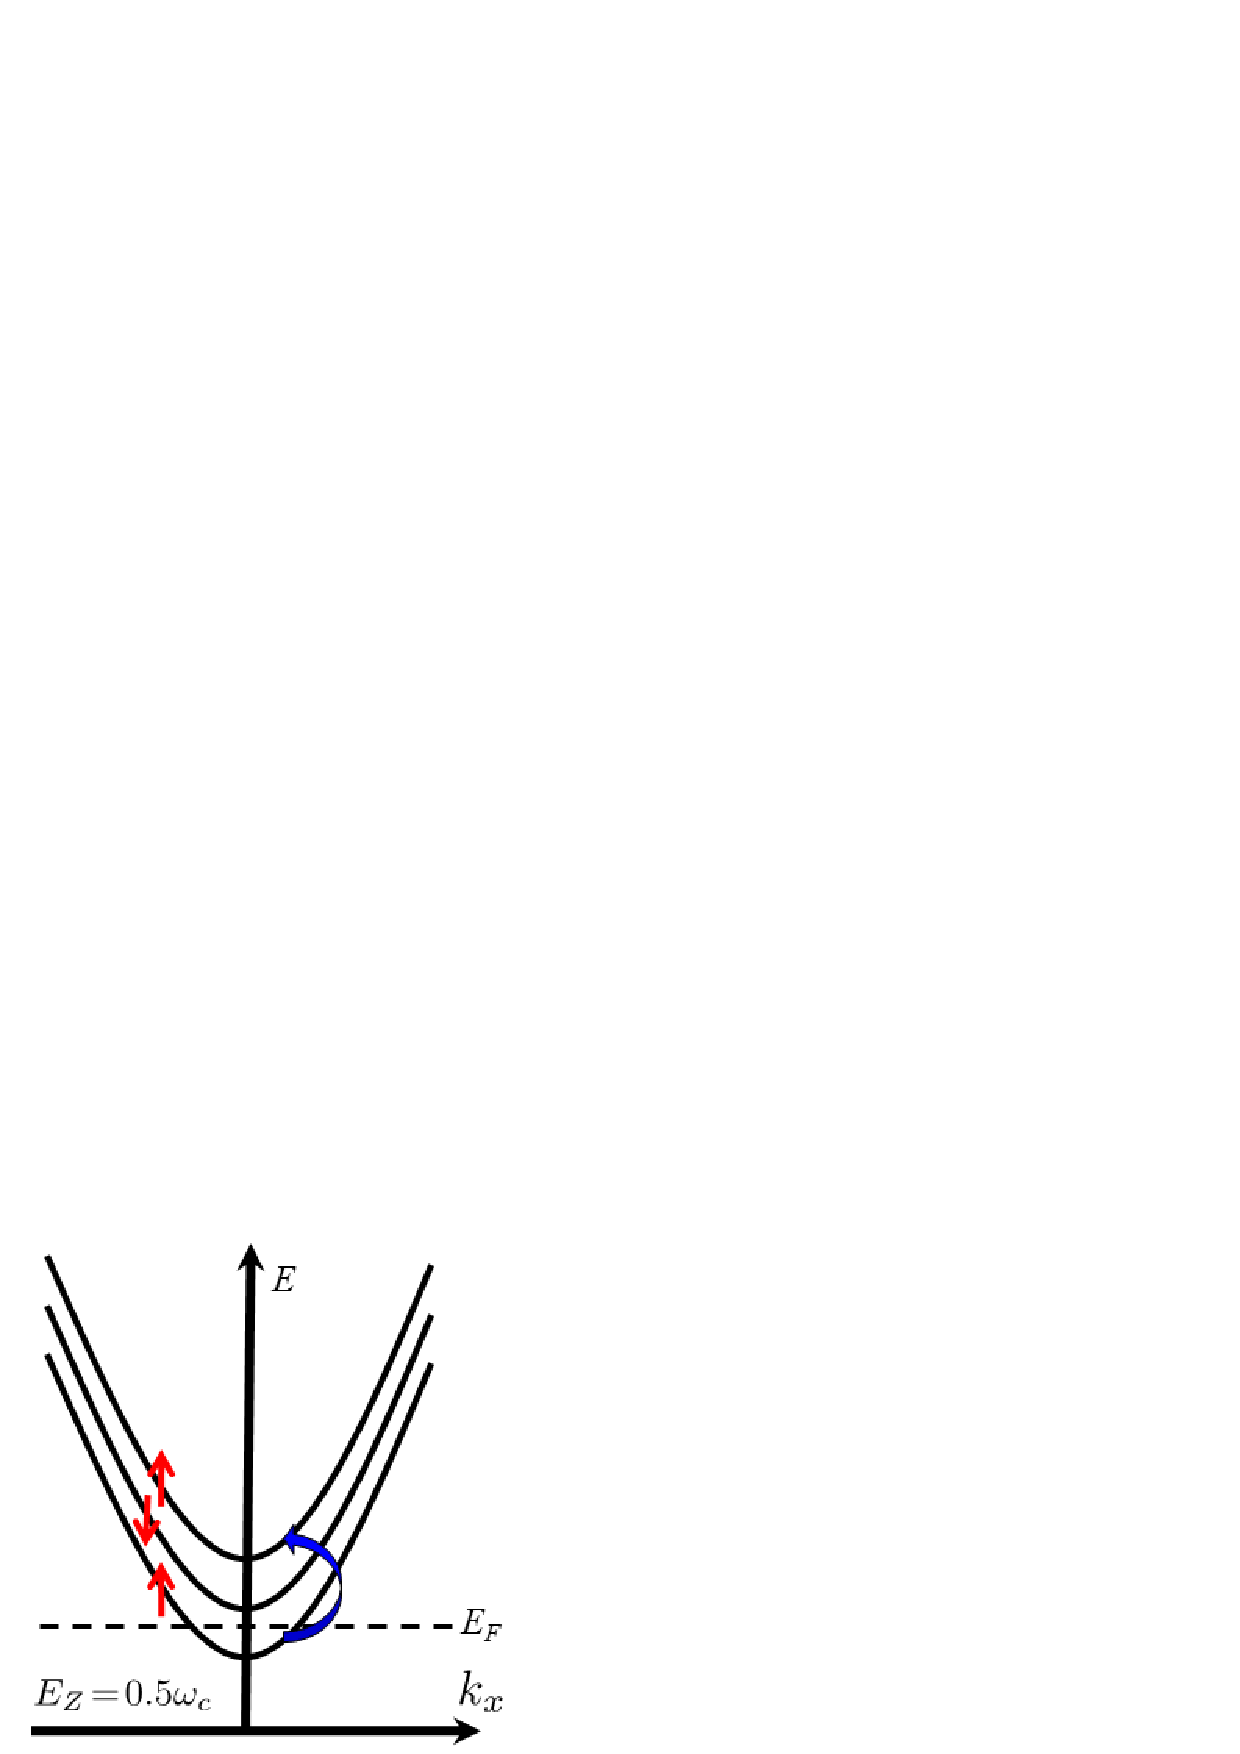
\includegraphics[width=0.7\columnwidth]{fig8.jpeg}
\caption{(color online) The three lowest energy subbands are $|0,+1\rangle$, $|0,-1\rangle$ and $|1,+1\rangle$.
The spin polarization is denoted by straight thin (red) arrows. 
Only the $|0,+1\rangle$ crosses the Fermi level, $E_F$.
The sloshing mode is the superposition of  p-h excitations from $|0,+1\rangle$ to $|1,+1\rangle$ subbands as indicated by a round thick (blue) arrow.\cite{Iqbal}}
\label{fig:par1}
\end{center}
\end{figure}



\begin{figure}[h]
\begin{center}
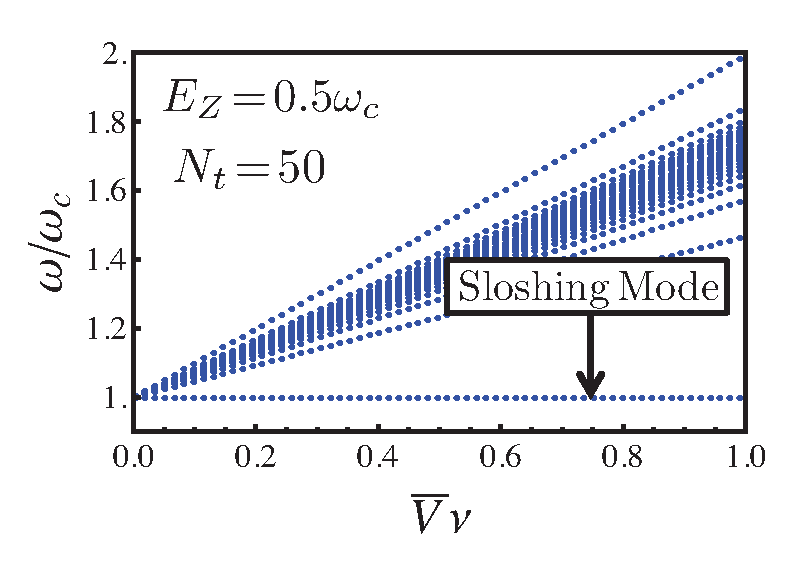
\includegraphics[width=0.6\columnwidth]{fig9.eps}
\caption{(color online) The dotted (blue) lines show the spectrum of collective modes that are the superpositions of p-h excitations between the subbands $|n+1,\pm1\rangle$ and $|n,\pm1\rangle$ as a function of the interaction parameter $\bar{V} \nu =(V_{\rho} - 3 V_s) \nu$.
The parameters used are (arb. units) $E_F = 50$,  $m=1$, $E_Z = 0.5 \omega_{\perp}$ and $\omega_{\perp} = 1$ corresponding to $N_t = 50$. 
The horizontal dotted line at $\omega/\omega_{\perp} =1$ demonstrates the Kohn theorem for sloshing mode.\cite{Iqbal}}
\label{fig:app_slosh}
\end{center}
\end{figure}




Here we demonstrate the consistency of the perturbation theory with the variants of Kohn theorem for the sloshing mode and spin precession mode.
We stress that although the perturbation theory holds for weak interaction the cancellation between the self-energy and vertex corrections holds exactly in every order of perturbation theory.
Such cancellation provides us with a test of the numerical calculations.

\section{Sloshing Mode}
Here we demonstrate the Kohn theorem for the sloshing mode in the presence of Zeeman splitting and electron-electron interaction, Eq.~\eqref{M19}.
The relevant p-h excitations are formed by the spin conserving transition between the adjacent subbands.
The electron and hole comprising such a pair reside at subbands $|n,\pm1\rangle$ and $|n+1,\pm 1\rangle$ respectively.

The most trivial is the situation with only the very lowest subband $|0,+1\rangle$ occupied, see Fig.~\ref{fig:par1}.
As only spin up species are present the short range interaction is ineffective for fermions, and the Kohn theorem is trivially satisfied.
Technically the contributions from the direct and exchange processes to both the self energy and the vertex corrections cancel.
The situation is less trivial for the large number of occupied levels.
In all cases the sloshing mode can be identified as the one not renormalized by interactions, see Fig.~\ref{fig:app_slosh}.

\begin{figure}[h]
\begin{center}
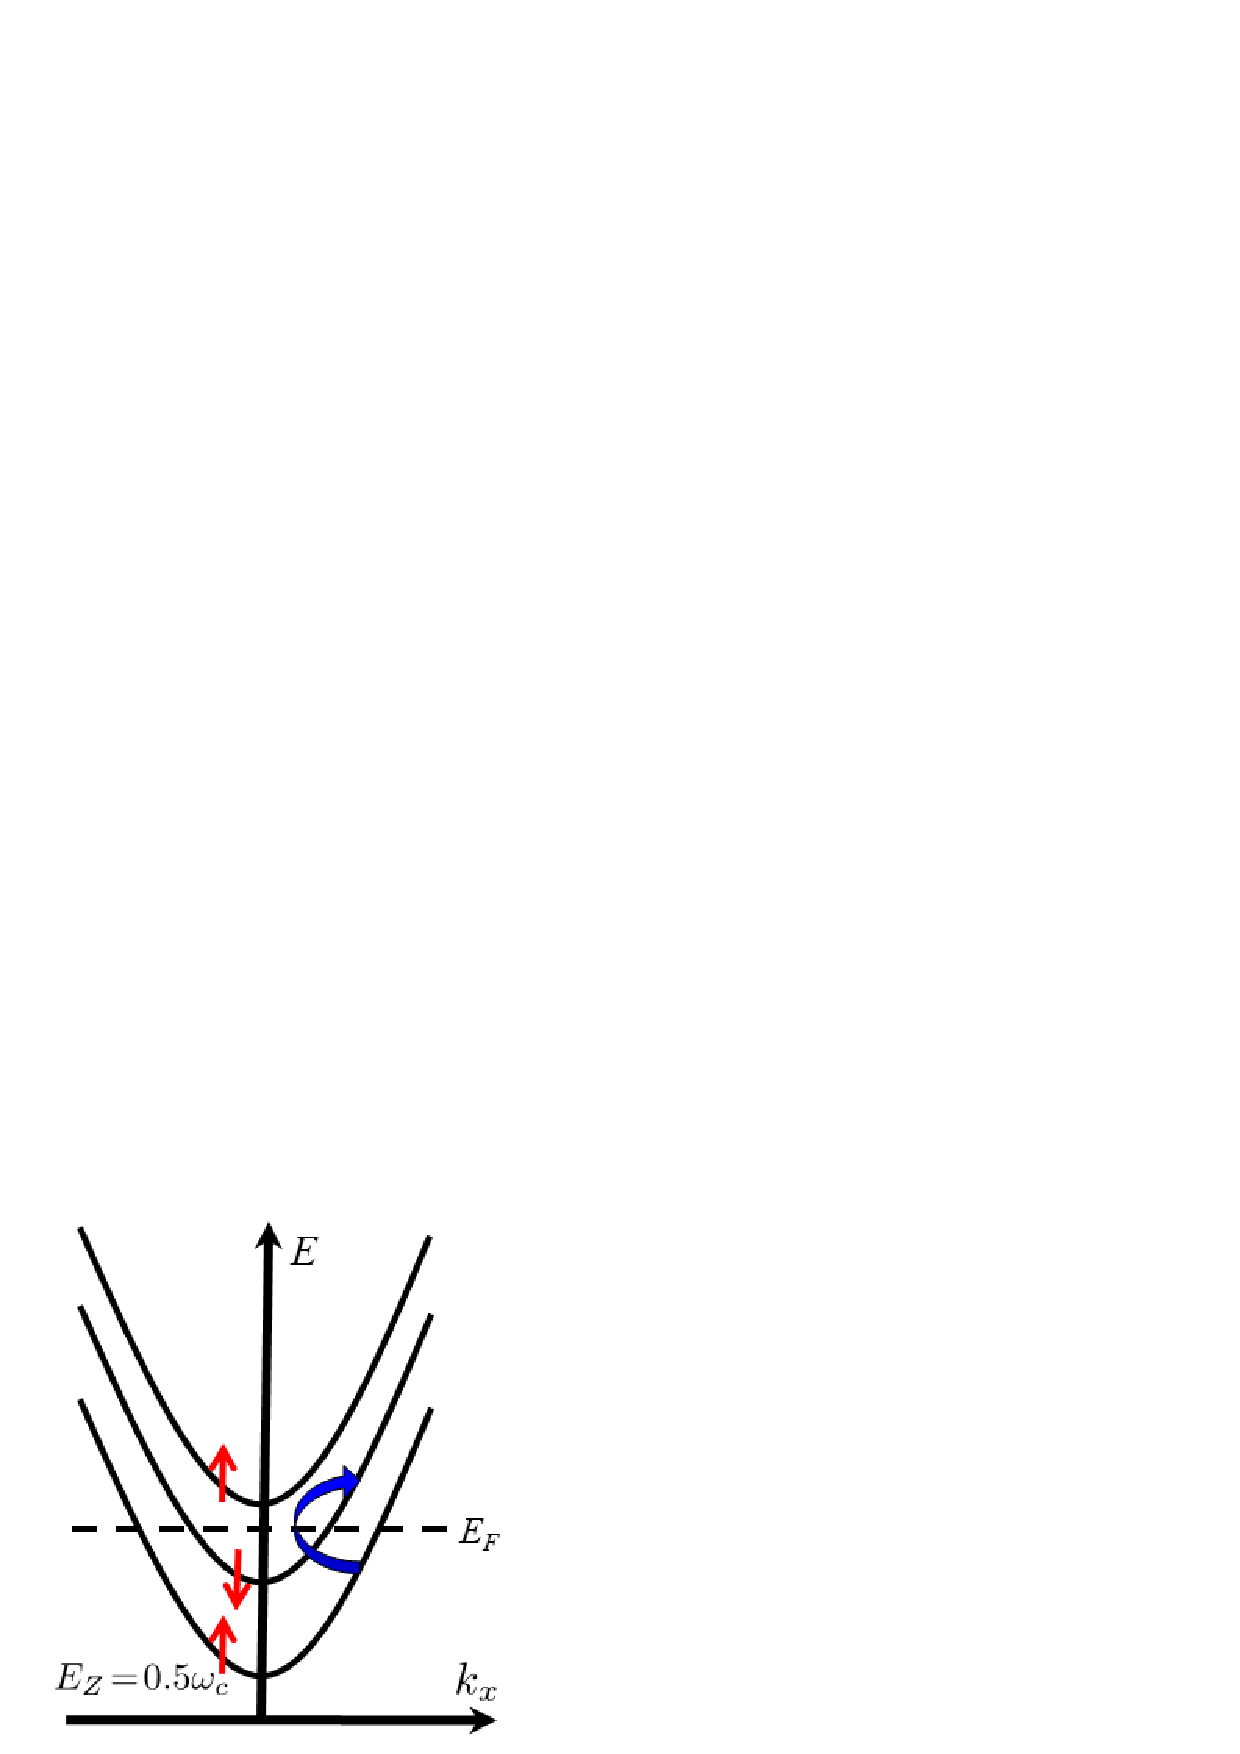
\includegraphics[width=0.4\columnwidth]{fig10.jpg}
\caption{(color online) The same three lowest energy subbands, $|0,+1\rangle$, $|0,-1\rangle$ and $|1,+1\rangle$ as in Fig.~\ref{fig:par1}.
The spin polarization is denoted by straight thin (red) arrows. 
The subbands $|0,+1\rangle$ and $|0,-1\rangle$ cross the Fermi level, $E_F$.
The spin precession mode is the superposition of  p-h excitations from $|0,+1\rangle$ to $|0,-1\rangle$ subbands as indicated by a round thick (blue) arrow.\cite{Iqbal}}
\label{fig:par2}
\end{center}
\end{figure}

\begin{figure}[t!]
\begin{center}
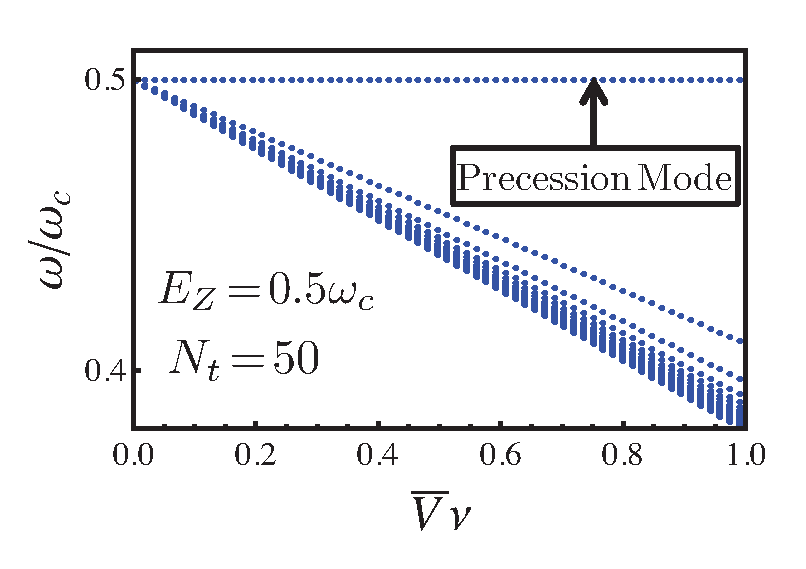
\includegraphics[width=0.6\columnwidth]{fig11.eps}
\caption{ (color online) The dotted (blue) lines show the spectrum of collective modes that are the superpositions of p-h excitations between the subbands $|n,+1\rangle$ and $|n,-1\rangle$ as a function of the interaction parameter $\bar{V} \nu =(V_{\rho} - 3 V_s) \nu$.
The parameters used are (arb. units) $E_F = 50$,  $m=1$, $E_Z = 0.5 \omega_{\perp}$ and $\omega_{\perp} = 1$ corresponding to $N_t = 50$. 
The horizontal dotted line at $\omega/ \omega_{\perp}=(\omega_{\perp} - E_Z)/\omega_{\perp} = 0.5 \omega_{\perp}$ demonstrates the Kohn theorem for spin precession mode.\cite{Iqbal}}
\label{fig:app_precession}
\end{center}
\end{figure}

\section{Spin-Precession Mode}
\label{sec:app_precession}
%
Here we make another generalization of the procedure developed in the Sec.~\ref{sec:Microscopic} to describe the effect of interactions on intra-band spin-flip transitions.
We start with the illustration of the Kohn theorem for the simplest case of two subbands occupied with Fermi momenta $k^F_{0,-1}$ and $k^F_{0,+1}$, see Fig.~\ref{fig:par2}. 
It is sufficient to focus on a single type of p-h excitations from subband $|0,+1 \rangle$ to subband $|0,-1 \rangle$.



In this case the proper generalization of the $\hat{\Gamma}$ matrix introduced in Eq.~\eqref{Gamma} has a single element,
\begin{align}\label{Gamma_app}
\Gamma(\omega) =\left[ \Pi^{-1}(\omega) + W \right]^{-1}\, ,
\end{align}
where we have for the polarization operator describing the excitations of p-h pairs shown in Fig.~\ref{fig:par2}, 
\begin{align}\label{Polarization1_app}
\Pi(\omega)= 
\frac{\pi^{-1} \left( k^F_{0,+1} - k^F_{0,-1}\right) }{
\omega  - E_Z
-
\Sigma_{0,-1} + \Sigma_{0,+1}
}
\end{align}
instead of Eq.~\eqref{Polarization1}.
The Fermi momenta and the self energies entering Eq.~\eqref{Polarization1_app} are defined by Eqs.~\eqref{kF} and \eqref{self1} respectively.
Instead of Eq.~\eqref{W} we have for the scattering vertex,
\begin{align}\label{W_app}
W =\bar{V} \ell^{-1} M^{0,0}_{0,0} \, .
\end{align}
It follow from Eq.~\eqref{Polarization1_app} that
\begin{align}\label{Polarization2_app}
\Pi^{-1}(\omega=E_Z)= 
\frac{\pi (\Sigma_{0,+1}-\Sigma_{0,-1})}{  k^F_{0,+1} - k^F_{0,-1}}\, .
\end{align}
Equation \eqref{self1} gives
\begin{align}\label{self1_app}
\Sigma_{0,\pm 1} & =
\bar{V} \ell^{-1}  \frac{k^F_{0,\mp 1}}{ \pi } M^{0,0}_{0,0}\, .
\end{align}
Combining Eqs.~\eqref{Gamma_app}, \eqref{W_app}, \eqref{Polarization2_app}, and \eqref{self1_app} we obtain
\begin{align}
\Gamma^{-1}(\omega = E_Z) = 0
\end{align}
which signifies the presence of the collective mode with unrenormalized frequency, $E_Z$ as expected.





The outlined derivation is easily generalized to arbitrary number of occupied subbands.
The condition analogous to Eq.~\eqref{det} leads to the spectrum of excitation shown in Fig.~\ref{fig:app_precession}.
The spin precession mode is identifiable as the one not renormalized by interactions.
Essentially similar approach has been used for the calculation of the spin wave dispersion in quantizing magnetic field with unequal occupation of Zeeman split Landau levels, (see Ref.~\cite{Kallin1984}).

%MK

% app1.tex (will be Appendix A)

%\label{app:proof}

%\newpage
%\section{Proof of Lemma~\ref{easylemma}}
%\label{app:proof:easy}

%\noindent \textbf{Proof}:\quad The result is clearly obvious.

%\setcounter{secnumdepth}{1}
%\setcounter{section}{0}
\chapter{Simple Examples of Collective Modes Frequencies in Presence of Interactions}
\section{Non-Local Interaction, $|n\rangle,|n+1\rangle$ Pair}
\label{Notes on unpublished calculations}
\setcounter{equation}{0}

\subsection{Calculation of Self-Energy}
We know,
\begin{equation}
G^{-1} = G_0^{-1} - \Sigma
\end{equation}
\begin{equation}
G = \frac{1}{{G_0^{-1}-\Sigma}}=\frac{G_0}{{1-G_0\Sigma}}=G_0(1+G_0\Sigma+G_0\Sigma G_0\Sigma)
\end{equation}
\begin{equation}
G=G_0 + G_0\Sigma G_0 + G_0\Sigma G_0\Sigma G_0
\end{equation}
We need to compute \(\Sigma\) to the leading order according to Fock approximation. \newline
The quantity, \[\delta
\langle\Psi\Psi^\dagger\rangle=\langle \Psi| -\int_0^\beta{d\tau\mathcal{H}_I}|\Psi^\dagger \rangle \]
\[\mathcal{H}_I=V\Psi^\dagger \Psi^\dagger \Psi \Psi \]
\[\delta\langle\Psi \Psi^\dagger \rangle = \langle \Psi| (-V) \Psi^\dagger \Psi^\dagger \Psi \Psi |\Psi^\dagger \rangle = -V \langle \Psi | \Psi^\dagger \Psi^\dagger \Psi \Psi | \Psi^\dagger \rangle = -V \langle \Psi \Psi^\dagger \rangle \langle \Psi \Psi^\dagger \rangle \langle \Psi \Psi^\dagger \rangle\]
\[\delta G = \delta \langle - \Psi \Psi^\dagger \rangle = (-)-V \langle -\Psi \Psi^\dagger \rangle \langle -\Psi \Psi^\dagger \rangle \langle -\Psi \Psi^\dagger \rangle (-1)^3 = V G_0 G_0 G_0 = \delta G\]

\begin{equation}
\Rightarrow \Sigma = -VG_0
\end{equation}
Thus, the sign is fixed. \newline \newline
In case of 2D gas,
\begin{equation}
\Sigma_{p,i\omega_n}=-\int{T\sum\limits_{\epsilon_n} V_q G_0(p+q,\epsilon_n+\omega_n)}
\end{equation}
In the (y,k) representation
\begin{equation}
G(y_1,y_2;k)=\sum\limits_m \frac{\Psi_m(y_1)\Psi_m^*(y_2)}{i\epsilon_n-E_{mk}}=\sum\limits_m \Psi_m(y_1)\Psi_m^*(y_2)G_m(\epsilon_n,k)
\end{equation}

\[E_{mk}=\omega_{\perp}(m+\frac{1}{2})+\frac{k^2}{2}; \; \; \; \xi_{mk}=E_{mk}-\mu\]

\begin{equation}
\begin{split}
\sum\limits_m(p,i\omega_n)=-\int{\frac{dq}{2\pi}T\sum\limits_{\epsilon_n}\sum\limits_{m'}}
& {\int{dy_1}\int{dy_2}} \\
& {V_q(y_1-y_2)\Psi_m(y_1)\Psi_{m'}(y_1)\Psi{m'}(y_2)\Psi_m(y2)\,G_m(\epsilon_n,k+q)e^{i\epsilon_n0^+}}
\end{split}
\end{equation}

\[T\sum\limits_{\epsilon_n}f(i\epsilon_n)=\oint_\Gamma\frac{dz}{2\pi i}f(z)n_F(z)\]

\[\frac{1}{e^{\beta z}+1};\ \ z=\frac{2\pi}{\beta}(n+\frac{1}{2})i+\delta z=z_n+\delta z\]

\[e^{\beta z}+1=e^{2\pi (n+\frac{1}{2})i+\delta z \beta}=(-1)e^{\beta\delta z}+1=-(1+\beta \delta z)+1=-\beta \delta z \]

\[\Rightarrow \frac{1}{e^{\beta z}+1}\approx \frac{1}{-\beta\delta z}=-\frac{1}{\beta}\frac{1}{\delta z}=-T\frac{1}{\delta z}\]

thus, \[T\sum\limits_{\epsilon_n}\frac{e^{i\epsilon_n0^+}}{i\epsilon_n-\xi}=-\oint_\Gamma\frac{dz}{2\pi i}n_F(z)\frac{e^{z0+}}{z-\xi}=\oint_{z=\xi}\frac{dz}{2\pi i}n_F(z)\frac{1}{z-\xi}=n_F(\xi)\]

or,
\begin{equation}
T\sum\limits_{\epsilon_n}\frac{e^{i\epsilon_n0^+}}{i\epsilon_n-\xi}=n_F(\xi)
\end{equation}

thus, \be \Sigma_m(p,i\omega_n)=-\int{\frac{dq}{2\pi} \sum\limits_{m'}\int{dy_1}\int{dy_2}V_q(y_1-y_2)\Psi_m(y_1)\Psi_{m'}(y_1)\Psi_{m'}(y_2)\Psi_m(y_2)n_F(\xi_{m',k+q})} \ee
we approximate the potential of the form
\be V_q(y_1-y_2)=V_0[cos(q_\perp(y_1-y_2))-1]\approx \frac{1}{2}V_0q_\perp^2(y_1-y_2)^2 \ee
as there is no dependence of V on momentum transferred along the guide, we can just integrate over
\[\int{\frac{dq}{2\pi}n_F(\xi_{m,k+q})}=\frac{2k_F^m}{2\pi}=\frac{k_F^m}{\pi}\]
which is the total number of electrons in the subband m.\\
Finally,
\be \Sigma_m(p,i\omega_n)=-\frac{1}{2}V_0q_\perp^2\sum\limits_{m'}\int{dy_1}\int{dy_2}(y_1-y_2)^2\frac{k_F^{m'}}{\pi}\Psi(y_1)\Psi_{m'}(y_1)\Psi_{m'}(y_2)\Psi(y_2) \ee

\subsection{Calculation of Polarization Operator}
let's first compute the following quantity:
\[T\sum\limits_m G_m(i\epsilon_n+i\omega_n,p+q)G(i\epsilon_n,p)\]
\[=\,T\sum\limits_n \frac{1}{i\epsilon_n+i\omega_n-\xi_1}\frac{1}{i\epsilon_n-\xi_2}\]
\[=\,-\oint_\Gamma \frac{dz}{2\pi i}n_F(z)\frac{1}{z+i\omega_n-\xi_1}\frac{1}{z-\xi_2}\]
\[=\,\frac{n_F(\xi_1-i\omega_n)}{\xi_1-\xi_2-i\omega_n}+\frac{n_F(\xi_2)}{\xi_2-\xi_1+i\omega_n}\]
\[=\,\frac{n_F(\xi_2)-n_F(\xi_1)}{\xi_2-\xi_1+i\omega_n}\]
now,
\[\Pi_{n-1}{n}=\,T\sum\limits_{\epsilon_n}\int{\frac{dp}{2\pi}G^n(i\epsilon_n+i\omega_n,p)G^{n-1}(i\epsilon_n,p)}\]
\[=\,\int{\frac{dp}{2\pi}\frac{n_F(\xi_p^{(n-1)})-n_F(\xi_p^n)}{\xi_p^{(n-1)}-\xi_p^n+i\omega_n}}\]
\[\xi_p^n=\;\frac{k^2}{2}+\omega_{\perp}(n+\frac{1}{2})+\Sigma_n\]

thus,
\be \Pi_{n-1}^n=\;\frac{1}{\pi}\frac{k_F^{n-1}-k_F^n}{-\omega_{\perp}-(\Sigma_n-\Sigma_{n-1})+i\omega_n} \ee

% \bd \includegraphics[scale=1]{slv11.jpg} \ed

\subsection{One Level Occupied}

\be \Sigma_0=- \piinv \C k_F^0 \ee

\be \Sigma_1= \piinv \C k_F^0 \ee

If we let $\omega \rightarrow \omega_{\perp}$,
\be \Pi_0^1 = \frac{1}{\pi} \frac{k_F^0}{\Sigma_0-\Sigma_1} = - \frac{\omega_{\perp}}{V_0q_\perp^2} \ee
Interaction, 
\be V=-\frac{1}{2}V_0q_\perp^2 ( \langle 1|y^2|1\rangle + \langle 0|y^2|0 \rangle) =-\frac{V_0q_\perp^2}{\omega_{\perp}} \ee
Thus, \be V\Pi = 1 \\ \ee


\subsection{Two Levels Occupied}
\be \Sigma_0= -\piinv \C (k_F^0-k_F^1) \ee
\be \Sigma_1 = -\piinv \C (-k_F^0+3k_F^1) \ee
\be \Sigma_2 = -\piinv \C (-2k_F^1) \ee
\be \Pi_1=\piinv \frac{k_F^0-k_F^1}{\Sigma_0-\Sigma_1}=\frac{k_F^0-k_F^1}{-\C (2k_F^0-4k_F^1)}\ee
\be\Pi_2=\piinv \frac{k_F^1-k_F^2}{\Sigma_1-\Sigma_2}=\frac{k_F^1}{-\C (-k_F^0+5k_F^1)} \ee
Thus, \be \Pi=-\frac{1}{\C} 
\left ( \begin{array}{cc}
\frac{k_F^0-k_F^1}{-\C (2k_F^0-4k_F^1)} & 0 \\
0 & \frac{k_F^1}{-\C (-k_F^0+5k_F^1)} \\
\end{array}
\right) \ee

\be V_{11}=-\frac{1}{2}V_0q_\perp^2(\langle 0|y^2|0 \rangle + \langle 1|y^2|1 \rangle ) = -\C.2\ee
\be V_{12}=-\frac{1}{2}V_0q_\perp^2(-1\langle 0|y|1\rangle \langle 1|y|2 \rangle)=\C.\sqrt{2}\ee
\be V_{22}=-\frac{1}{2}V_0q_\perp^2(\langle 1|y^2|1 \rangle + \langle 2|y^2|2 \rangle ) = -\C.4 \ee
\be V=-\C \left (\begin{array}{cc} 2 & -\sqrt{2} \\ -\sqrt{2} & 4 \\ \end{array} \right) \ee
Simple calculation yields: \be det[\mathbbm{1}-V\Pi]=0 \\ \ee

\subsection{Three Levels Occupied}
\be \Sigma_0= -\piinv \C (k_F^0 -k_F^1) \, (Same\ as\ before)\ \ee
\be \Sigma_1\ has\ an\ additional\ part:\ =\piinv\C.2k_F^2 \ee
\be \Rightarrow\Sigma_1=-\piinv\C(-k_F^0+3k_F^1-2k_F^2) \ee
\be \Sigma_2\ has\ an\ additional\ part:\ =-\piinv\C(-2k_F^1+5k_F^2) \ee
\be \Sigma_3=-\piinv\C(-3k_F^2) \ee

\be \Pi_0=\piinv\frac{k_F^0-k_F^1}{\Sigma_0-\Sigma_1}=\frac{k_F^0-k_F^1}{-\C(2k_f^0-4k_F^1+2k_F^2)} \ee
\be \Pi_1=\piinv\frac{k_F^1-k_F^2}{\Sigma_1-\Sigma_2}=\frac{k_F^1-k_F^2}{-\C(-k_F^0+5k_F^1-7k_F^2)} \ee
\be \Pi_2=\piinv\frac{k_F^2-k_F^3}{\Sigma_2-\Sigma_3}=\frac{k_F^2}{-\C(-2k_F^1+8k_F^2)} \ee
Thus, \be \\ \Pi=\left(\begin{array}{ccc}
									\frac{k_F^0-k_F^1}{-\C(2k_f^0-4k_F^1+2k_F^2)} & 0 & 0\\
									0 & \frac{k_F^1-k_F^2}{-\C(-k_F^0+5k_F^1-7k_F^2)} & 0\\
									0 & 0 & \frac{k_F^2}{-\C(-2k_F^1+8k_F^2)} \end{array} \right ) \ee
\be V_{11}=-\C.2\ (as\ before) \ee
\be V_{12}=\C.\sqrt{2}=V_{21}\ (as\ before)\ \ee
\be V_{13}=0=V_{31}\ee
\be V_{22}=-\C.4\ (as\ before) \ee
\be V_{23}=-\frac{1}{2}V_0q_\perp^2(-2\langle 2|y|3 \rangle \langle 1|y|2 \rangle)=\C.\sqrt{6}=V_{32} \ee
\be V_{33}=-\frac{1}{2}V_0q_\perp^2(\langle 3|y^2|3 \rangle + \langle 2|y^2|2 \rangle)=-\C.6 \ee
\be V=-\C \left (\begin{array}{ccc}
							2 & -\sqrt{2} & 0 \\
							-\sqrt{2} & 4 & -\sqrt{6} \\
							0 & -\sqrt{6} & 6 \end{array} \right ) \ee
After simple calculation, \be \det[\mathbbm{1}-V\Pi]=0 \ee




\section{Non-Local Interaction, $|n,\uparrow\rangle, |n,\downarrow\rangle$ Pair}

\begin{equation}
	H=\frac{p_x^2+p_z^2}{2m_e}+V_c(z)-\frac{1}{2}E_z\sigma_z
\end{equation}
\newline
where,
\begin{equation}
	E_{m,s,k}=\frac{k^2}{2m_e}+(m+\frac{1}{2})\omega_{\perp}-\frac{1}{2}E_zs
\end{equation}

\begin{equation}
G_{m,s}(p,i\omega_n)=\frac{1}{i\omega_n+i\epsilon_n-\xi_{m,s}(p)-\Sigma_{m,s}}
\end{equation}
\newline
Self energies:
\begin{equation}
	\Sigma_{m,s}(p,i\omega_n)=-\int\frac{dq}{2\pi}T\Sigma_{\epsilon_n}\Sigma_{m'}V_q(y_1-y_2)\phi_m(y_1)\phi_{m'}(y_1)\phi_{m'}(y_2)\phi_m(y_2)\frac{e^{i\epsilon_n0^+}}{i\epsilon_n-\xi_{m,s}(p)}
\end{equation}

\[T\sum\limits_{\epsilon_n}\frac{e^{i\epsilon_n0^+}}{i\epsilon_n-\xi_{m,s}(p)}=n_F(\xi_{m,s}(p))\]

\[V(y_a-y_2)=V_0(cos(q_\perp(y_a-y_2))-1\approx\frac{1}{2}V_0q_\perp^2(y_1-y_2)^2\]

\begin{equation}
	\Sigma{m,s}=-\frac{1}{2\pi}V_0 q_\perp^2\sum\limits_{m'}\int{dy_1dy_2}{(y_1-y_2)^2k_F^{m',s}\phi_m(y_1)\phi_m'(y_1)\phi_{m'}(y_2)\phi_m(y_2)}
\end{equation}


Polarization Operator:
\begin{figure}[h]
\begin{center}
	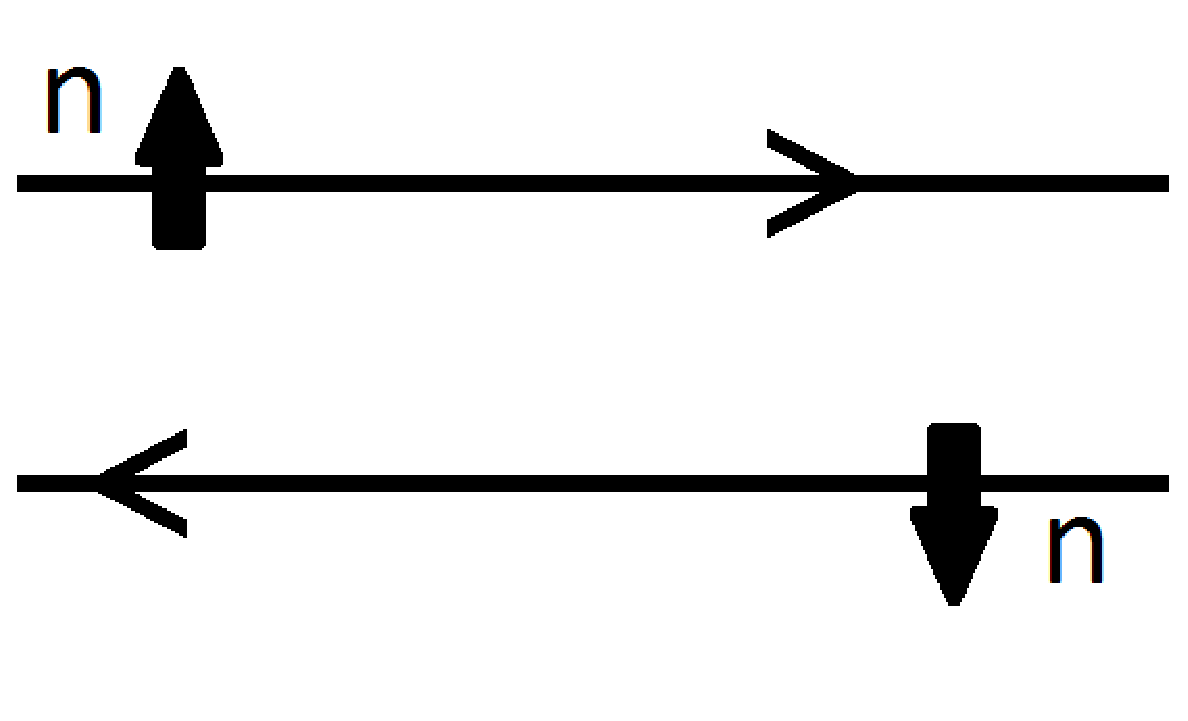
\includegraphics[width=1in]{apfig1}
\end{center}
\end{figure}
\[T\sum\limits_{\epsilon_n}G_{m,s}(i\epsilon_n+i\omega_n,p)G_{m',s'}(i\epsilon_n,p)\]

\[= T\sum\limits_{\epsilon_n} \frac{1}{i\epsilon_n+i\omega_n-\xi_{m,s}(p)-\Sigma_{m,s}} \frac{1}{i\epsilon_n-\xi{m',s'}(p)-\Sigma_{m',s'}}\]

\[=-\oint_\Gamma \frac{dz}{2\pi i} n_F(z) \frac{1}{z+i\omega_n-\xi_{m,s}(p)-\Sigma_{m,s}} \frac{1}{z-\xi_{m',s'}(p)-\Sigma_{m',s'}}\]

\[=\frac{n_F(\xi_{m',s'})-n_F(\xi_{m,s})}{\xi_{m',s'}-\xi_{m,s}+\Sigma_{m',s'}-\Sigma_{m,s}}\]

\[\Pi_{n,\downarrow}^{n,\uparrow}=T\sum\limits_{\epsilon_n} \int \frac{dp}{2\pi} G_{n,\uparrow}(i\epsilon_n+i\omega_n,p)G_{n,\downarrow}(i\epsilon_n,p)\]
or,
\begin{equation}
	\Pi_n=\frac{1}{\pi} \frac{k_F^{n,\downarrow}-k_F^{n,\uparrow}}{i\omega_n-E_z+\Sigma_{n,\downarrow}-\Sigma_{n,\uparrow}}
\end{equation}

Vertex correction:

\[\]

\begin{figure}[h]
	\centering
	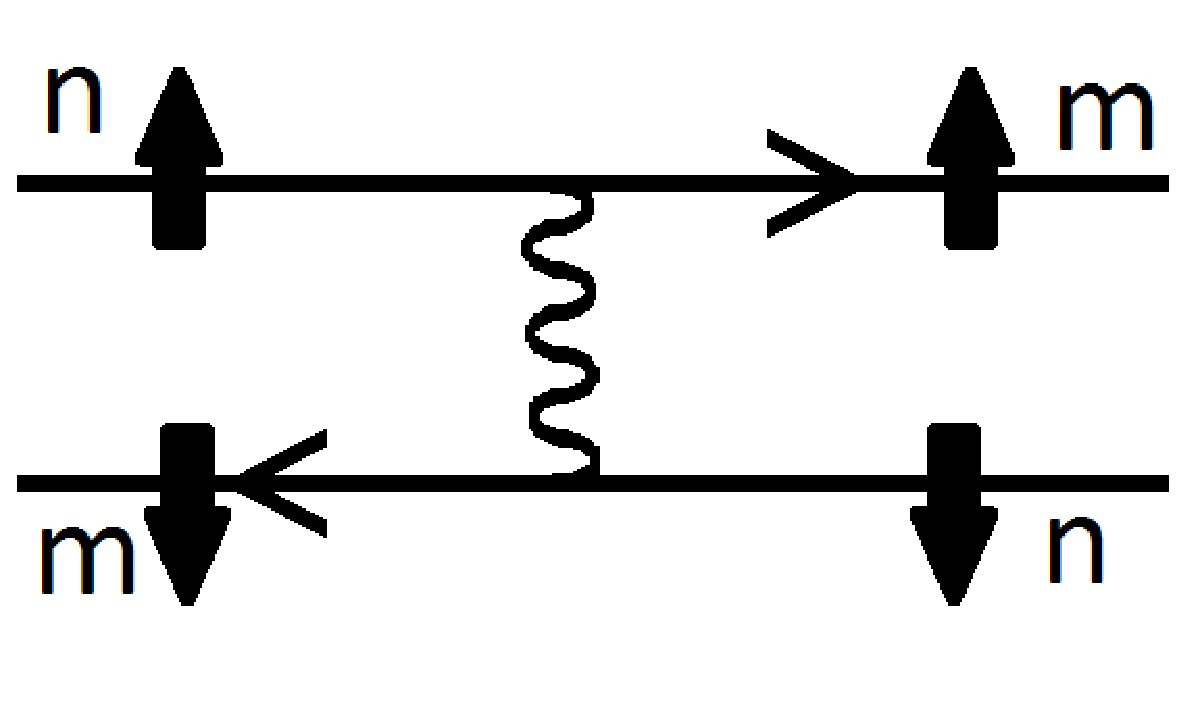
\includegraphics[width=1in]{apfig2}
\end{figure}

\begin{equation}
	V=\frac{1}{2} V_0 q_\perp^2 \int \phi_n(y_1) \phi_m(y_1) (y_1-y_2)^2 \phi_m(y_2) \phi_n(y_2) dy_1 dy_2
\end{equation}

\subsection{One Level Occupied}

\[\Sigma_{0,\uparrow}=-\frac{1}{2\pi} V_0 q_\perp^2 k_F^{0,\uparrow}.2\langle 0|y^2|0\rangle=-\frac{1}{2\pi} \frac{V_0 q_\perp^2}{\omega_{\perp}} k_F^{0,\uparrow}\]

\[\Sigma_{0,\downarrow}=-\frac{1}{2\pi} V_0 q_\perp^2 k_F^{0,\downarrow}.2\langle0|y^2|0\rangle = -\frac{1}{2\pi} \frac{V_0 q_\perp^2}{\omega_{\perp}} k_F^{0,\downarrow}\]


\[\Pi|_{\omega\rightarrow E_z}=\frac{\frac{1}{\pi}(k_F^{0,\downarrow}-k_F^{0,\uparrow})}{\Sigma_{0,\downarrow}-\Sigma_{0,\uparrow}}=\frac{\frac{1}{\pi}(k_F^{0,\downarrow}-k_F^{0,\uparrow})}{-\frac{1}{2\pi} \frac{V_0 q_\perp^2}{\omega_{\perp}}(k_F^{0,\downarrow}-k_F^{0,\uparrow})}=-\frac{2\omega_{\perp}}{V_0 q_\perp^2}\]

\[V=\frac{1}{2} V_0 q_\perp^2. 2\langle 0|y^2|0\rangle = \frac{V_0 q\perp^2}{2\omega_{\perp}} \]

\[\mathbb{I}+V\Pi=1-1=0\]

\subsection{Two Levels Occupied}

\[\Sigma_{0,\uparrow}=-\frac{1}{2\pi} V_0 q_\perp^2 \{k_F^{0,\uparrow}.2\langle 0|y^2|0\rangle + k_F^{1,\uparrow}.(-2)|\langle 0|y|1\rangle|^2\}=-\frac{1}{2\pi} \frac{V_0 q_\perp^2}{\omega_{\perp}}(k_F^{0,\uparrow}-k_F^{1,\uparrow})\]

Similarly,
\[\Sigma_{0,\downarrow}=-\frac{1}{2\pi} \frac{V_0 q_\perp^2}{\omega_{\perp}} (k_F^{0,\downarrow}-k_F^{1,\downarrow})\]

\[\Sigma_{1,\uparrow}=-\frac{1}{2\pi} V_0 q_\perp^2 \{k_F^{1,\uparrow}.2\langle 1|y^2|1\rangle + k_F^{0,\uparrow}.(-2) |\langle 0|y|1\rangle|^2 \} = -\frac{1}{2\pi} \frac{V_0 q_\perp^2}{\omega_{\perp}} (3k_F^{1,\uparrow}-k_F^{0,\uparrow})\]

Similarly, 
\[\Sigma_{1,\downarrow}=-\frac{1}{2\pi} \frac{V_0 q_\perp^2}{\omega_{\perp}} (3k_F^{1,\downarrow}-k_F^{0,\downarrow})\]

\[\Pi_1|_{\omega\rightarrow E_z}=-\frac{2\omega_{\perp}}{V_0 q_\perp^2} \frac{k_F^{0,\downarrow}-k_F^{0,\uparrow}}{k_F^{0,\downarrow}-k_F^{0,\uparrow}-k_F^{1,\downarrow}+k_F^{1,\uparrow}}\]

\[\Pi_2|_{\omega\rightarrow E_z}=-\frac{2\omega_{\perp}}{V_0 q_\perp^2} \frac{k_F^{1,\downarrow}-k_F^{1,\uparrow}}{3k_F^{1,\downarrow}-3k_F^{1,\uparrow}-k_F^{0,\downarrow}+k_F^{0,\uparrow}}\]

\[\Pi=-\frac{2\omega_{\perp}}{V_0 q_\perp^2} 
\left(\begin{matrix}
	\frac{k_F^{0,\downarrow}-k_F^{0,\uparrow}}{k_F^{0,\downarrow}-k_F^{0,\uparrow}-k_F^{1,\downarrow}+k_F^{1,\uparrow}} & 0 \\
	0 & \frac{k_F^{1,\downarrow}-k_F^{1,\uparrow}}{3k_F^{1,\downarrow}-3k_F^{1,\uparrow}-k_F^{0,\downarrow}+k_F^{0,\uparrow}}
\end{matrix}\right)\]

\[V_{11}=\frac{V_0 q_\perp^2}{2\omega_{\perp}}; V_{12}=\frac{1}{2} V_0 q_\perp^2 (-2) |\langle 0|y|1\rangle|^2=-\frac{V_0 q_\perp^2}{2\omega_{\perp}}=V_{21} \]

\[V_{22}=\frac{1}{2} V_0 q_\perp^2.2.\langle 1|y^2|1\rangle=3.\frac{V_0 q_\perp^2}{2\omega_{\perp}}\]

\[V=\frac{V_0 q_\perp^2}{2\omega_{\perp}} \left(
	\begin{matrix}
		1 & -1 \\
		-1 & 3
	\end{matrix} \right) \]
	
After calculation,
\[ det(\mathbb{I}+V\Pi)=0 \]

\subsection{Three Levels Occupied}

\[\Sigma_{0,\uparrow}=-\frac{1}{2\pi} \frac{V_0 q_\perp^2}{\omega_{\perp}} (k_F^{0,\uparrow}-k_F^{1,\uparrow})\]

\[\Sigma_{0,\downarrow}=-\frac{1}{2\pi} \frac{V_0 q_\perp^2}{\omega_{\perp}} (k_F^{0,\downarrow}-k_F^{1,\downarrow})\]

\begin{align*}
\Sigma_{1,\uparrow} &=-\frac{1}{2\pi} V_0 q_\perp^2 \{k_F^{1,\uparrow}.2\langle 1|y^2|1\rangle + k_F^{0,\uparrow}.(-2) |\langle 0|y|1\rangle|^2 + k_F^{2,\uparrow}.(-2)|\langle 1|y|2\rangle|^2\} \\
 &= -\frac{1}{2\pi} \frac{V_0 q_\perp^2}{\omega_{\perp}} (-k_F^{0,\uparrow}+3k_F^{1,\uparrow}-2k_F^{2,\uparrow})
\end{align*}

Similarly, 
\[\Sigma_{1,\downarrow}=-\frac{1}{2\pi} \frac{V_0 q_\perp^2}{\omega_{\perp}} (-k_F^{0,\downarrow}+3k_F^{1,\downarrow}-2k_F^{2,\downarrow})\]

\[\Sigma_{2,\uparrow}=-\frac{1}{2\pi} V_0 q_\perp^2 \{k_F^{1,\uparrow}.(-2)|\langle 1|y|2\rangle|^2 + k_F^{2,\uparrow}.2\langle 2|y^2|2\rangle\} = -\frac{1}{2\pi} \frac{V_0 q_\perp^2}{\omega_{\perp}} (-2k_F^{1,\uparrow}+5k_F^{2,\uparrow})\]

Similarly,
\[\Sigma_{2,\downarrow}= -\frac{1}{2\pi} \frac{V_0 q_\perp^2}{\omega_{\perp}} (-2k_F^{1,\downarrow}+5k_F^{2,\downarrow})\]

\[\Pi=\left(
	\begin{matrix}
		\Pi_1 & 0 & 0\\
		0 & \Pi_2 & 0\\
		0 & 0 & \Pi_3 \end{matrix} \right) \]
where,
\[\Pi_1=-\frac{2\omega_{\perp}}{V_0 q_\perp^2} \frac{k_F^{0,\downarrow}-k_F^{0,\uparrow}}{k_F^{0,\downarrow}-k_F^{1,\downarrow}-k_F^{0,\uparrow}+k_F^{1,\uparrow}}\]

\[\Pi_2=-\frac{2\omega_{\perp}}{V_0 q_\perp^2} \frac{k_F^{1,\downarrow}-k_F^{1,\uparrow}}{-k_F^{0,\downarrow}+3k_F^{1,\downarrow}-sk_F^{2,\downarrow}+k_F^{0,\uparrow}-3k_F^{1,\uparrow}+2k_F^{2,\uparrow}}\]

\[\Pi_3=-\frac{2\omega_{\perp}}{V_0 q_\perp^2} \frac{k_F^{2,\downarrow}-k_F^{2,\uparrow}}{-2k_F^{1,\downarrow}+5k_F^{2,\downarrow}+2k_F^{1,\uparrow}-5k_F^{2,\uparrow}}\]

And,

\[V_{11}=\frac{V_0 q_\perp^2}{2\omega_{\perp}}\]
\[V_{12}=V_{21}=-\frac{V_0 q_\perp^2}{2\omega_{\perp}}\]
\[V_{22}=3.\left(\frac{V_0 q_\perp^2}{2\omega_{\perp}}\right)\]
\[V_{23}=V_{32}=\frac{1}{2} V_0 q_\perp^2.(-2) |\langle 1|y|2\rangle|^2=-2\left(\frac{V_0 q_\perp^2}{2\omega_{\perp}}\right)\]
\[V_{13}=V_{31}=0\]
\[V_{33}=\frac{1}{2} V_0 q_\perp^2.2\langle 2|y^2|2\rangle = 5.\left(\frac{V_0 q_\perp^2}{2\omega_{\perp}}\right)\]

\[V=\frac{V_0 q_\perp^2}{2\omega_{\perp}} \left(\begin{matrix}
		1 & -1 & 0\\
		-1 & 3 & -2\\
		0 & -2 & 5 \end{matrix}\right)\]
		
After calculation, \[det(\mathbb{I}+V\Pi)=0\]

\section{Non-Local Interaction, $|n+1,\uparrow\rangle ,|n,\downarrow\rangle$ Pair}

\subsection{One Level Occupied}

\[\Sigma_{0,\downarrow}=-\frac{1}{2\pi} V_0 q_\perp^2. 2\langle 0|y^2|0 \rangle k_F^{0,\downarrow} = -\frac{1}{2\pi} \frac{V_0 q_\perp^2}{\omega_{\perp}}k_F^{0,\downarrow}\]

\[\Sigma_{1,\uparrow}=-\frac{1}{2\pi} \frac{V_0 q_\perp^2}{\omega_{\perp}} \{k_F^{1,\uparrow}.2\langle 1|y^2|1\rangle + k_F^{0,\uparrow}.(-2)|\langle 0|y|1\rangle|^2\} = -\frac{1}{2\pi} \frac{V_0 q_\perp^2}{\omega_{\perp}} (3k_F^{1,\uparrow}-k_F^{0,\uparrow})\]

\begin{figure}[h]
	\centering
	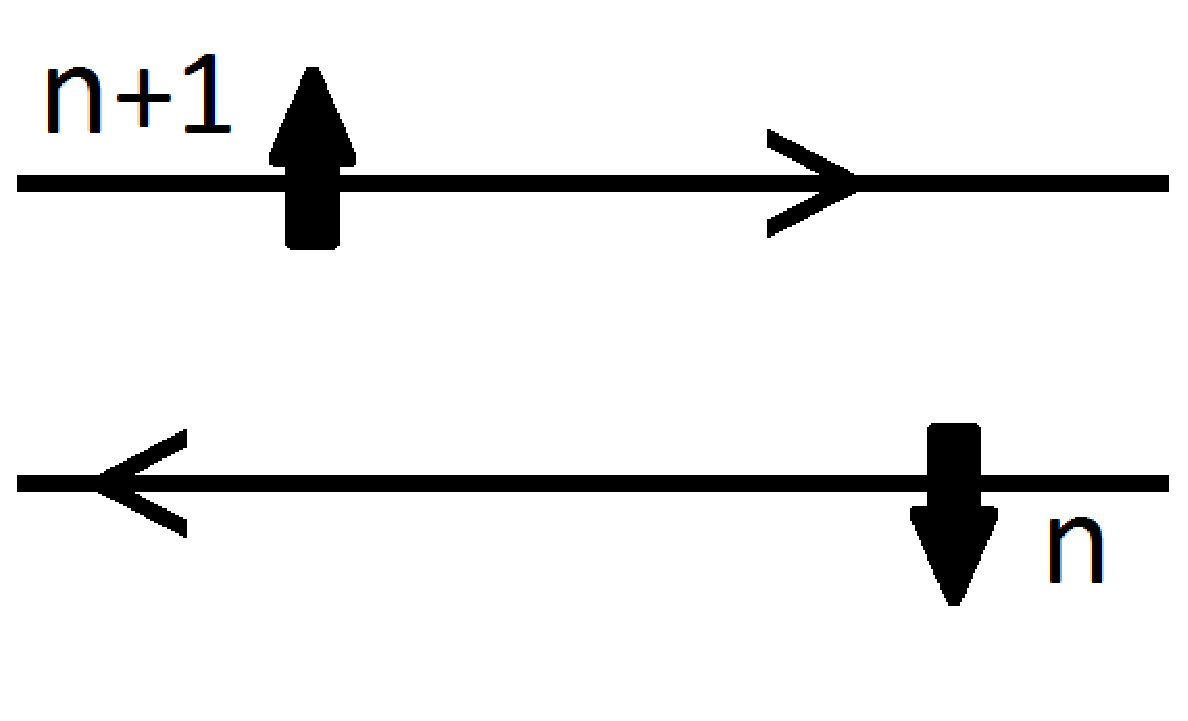
\includegraphics[width=1in]{apfig3}
\end{figure}

\[\Pi=\frac{k_F^{0,\downarrow}-k_F^{1,\uparrow}}{i\omega_n-(\omega_{\perp}-E_z)-\frac{1}{2\pi} \frac{V_0 q_\perp^2}{\omega_{\perp}} (k_F^{0,\downarrow}+k_F^{0,\uparrow}-3k_F^{1,\uparrow})}\]

\begin{figure}[h]
	\centering
	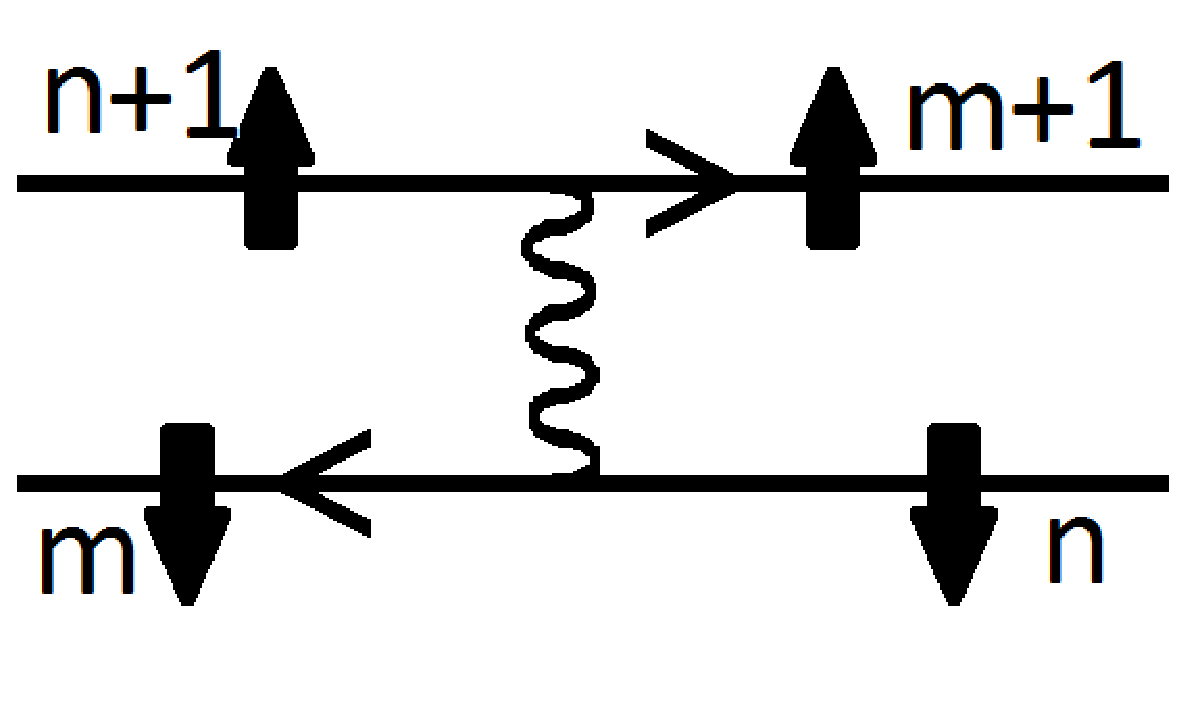
\includegraphics[width=1in]{apfig4}
\end{figure}

\[V=\frac{1}{2} V_0 q_\perp^2 \left( \langle 0|y^2|0\rangle + \langle 1|y^2|1\rangle \right) = \frac{1}{2} \frac{V_0 q_\perp^2}{\omega_{\perp}} (2)\]

\[V.\Pi|_{\omega\rightarrow (\omega_{\perp}-E_z)}=\frac{(k_F^{0,\downarrow}-k_F^{1,\uparrow}) . \frac{V_0 q_\perp^2}{\omega_{\perp}}}{-\frac{1}{2\pi} \frac{V_0 q_\perp^2}{\omega_{\perp}} (k_F^{o,\downarrow}+k_F^{0,\uparrow}-3k_F^{1,\uparrow})}\neq -1\]

\[det(\mathbb{I}+V\Pi)|_{\omega\rightarrow (\omega_{\perp}-E_z)}\neq0\]

\section{Local Interaction, $|n+1,\uparrow\rangle,|n,\downarrow\rangle$ Pair}

\[V\equiv V_0 \delta(y_1-y_2)\]

\[\Sigma_{n,\downarrow}=(V_\rho-3V_s)\sum\limits_{m=0}^N\frac{k_F^{m,\uparrow}}{\pi}\int\phi_n^2(y)\phi_m^2(y)dy\]

\[\Sigma_{n+1,\uparrow}=(V_\rho-3V_s)\sum\limits_{m=0}^{N+1}\frac{k_F^{m,\downarrow}}{\pi}\int\phi_{n+1}^2(y)\phi_m^2(y)dy\]

\[\Pi_n=\frac{\frac{1}{\pi}(k_F^{n,\downarrow}-k_F^{n+1,\uparrow})}{i\omega_n-(\omega_{\perp}-E_z)+\Sigma_{n,\downarrow}-\Sigma_{n+1,\uparrow}}\]

\[V=(V_\rho-3V_s)\int\phi_{n+1}\phi_{m+1}\phi_n\phi_m dy\]

%%%%%%%%%%%%%%%%%%%%%%%%%%%%%%%%%%%%%%%%%%%%%%%%%%%%%%%%%%%%%%%%%%%%%%%%%%
% Spin-Orbit%%%%%%%%%%%%%%%%%%%%%%%%%%%%%%%%%%%%%%%%%%%%%%%%%%%%%%%%%%%%%%
%%%%%%%%%%%%%%%%%%%%%%%%%%%%%%%%%%%%%%%%%%%%%%%%%%%%%%%%%%%%%%%%%%%%%%%%%%

\section{Local Interaction with SO coupling}

The Hamiltonian:

\begin{equation}
	H= \frac{p_x^2+p_y^2}{2m_e} +V_c(y)- \frac{1}{2} E_z \sigma_z + \alpha_- p_y \sigma_x
\end{equation}

The eigenstates and eigenvectors are:

\begin{equation}
	\begin{split}
		&|\psi_{n,+}\rangle = \alpha_n |\phi_{n+1}^+\rangle + \beta_n |\phi_n^-\rangle \\
	&|\psi_{n,-}\rangle = \beta_n^* |\phi_{n+1}^+\rangle - \alpha_n^* |\phi_n^-\rangle
	\end{split}
\end{equation}

where,
\[\alpha_n=i cos\left(\frac{\theta_n}{2}\right),\ \beta_n=-sin\left(\frac{\theta_n}{2}\right),\ \theta_n =cos^{-1}\left[\frac{E_z-\omega_{\perp}}{\sqrt{(E_z-\omega_{\perp})^2+\left[\delta_n^{SO}\right]^2}}\right] \]
%%%%%%%%%%%%%%%%%%%%%%%%%%%%%%%%%%%%%%%%%%%%%%%%%%%%%%%%%%%%%%%%%%%%%%%%%%%%%%%%%%%%%
%%%%%%%%%%%%%%%%%%%%%%%%%%%%%%%%%%%%%%%%%%%%%%%%%%%%%%%%%%%%%%%%%%%%%%%%%%%%%%%%%%%%%
%%%%%%%%%%%%%%%%%%%%%%%%%%%%%%%%%%%%%%%%%%%%%%%%%%%%%%%%%%%%%%%%%%%%%%%%%%%%%%%%%%%%%

\section{The Equation of the``Theory" Curve}

We have, 

\be F_0=\frac{1}{2} (V_\rho-3V_s) N(0) \equiv \frac{1}{2} \overline{V} \frac{m}{\pi} \ee

\be G_0=-\frac{1}{2} (V_\rho-3V_s) N(0) \equiv -\frac{1}{2} \overline{V} \frac{m}{\pi} \ee

Thus, $F_0=-G_0 \\$

Then we have,

\[ \omega_{th}=\pm \left[ {E_z + E_z \frac{G_1-G_0}{2(1+G_0)} - \sqrt{E_z^2 \frac{(G_1-G_0)^2}{4(1+G_0)^2}+\omega_{\perp}^2 \frac{G_1+1}{F_1+1} \frac{G_0+1}{F_0+1}}} \right] \]
\be \Rightarrow \omega_{th}= \pm \left[ {E_z + E_z \frac{\overline{V}\frac{m}{\pi}}{4\left(1-\frac{1}{2}\overline{V}\frac{m}{\pi}\right)}-\sqrt{E_z^2 \frac{\left( \overline{V} \frac{m}{\pi} \right)^2}{16\left(1-\frac{1}{2}\overline{V}\frac{m}{\pi}\right)^2}+\omega_{\perp}^2\left( \frac{1-\frac{1}{2}\overline{V}\frac{m}{\pi}}{1+\frac{1}{2}\overline{V}\frac{m}{\pi}}\right)} } \right]\ee

\section{Eigenvalue Scheme for Computation (for $|n+1,\uparrow\rangle , |n,\downarrow\rangle$ Pair)}

We are interested in the zeroes of the matrix $\left[ \Pi^{-1}+V \right]$, which is:

\begin{align*}
& \left[ \Pi^{-1}+V \right]_{nn'} \\ 
= &\frac{\omega-(\omega_{\perp}-E_z)+\frac{\overline{V}}{\pi} \sum\limits_m \left( \frac{k_F^{m,\uparrow}}{\pi}\int\phi_n^2(y)\phi_m^2(y)dy - \frac{k_F^{m,\downarrow}}{\pi}\int\phi_{n+1}^2(y)\phi_m^2(y)dy \right)}{\frac{1}{\pi} \left( k_F^{n,\downarrow}-k_F^{n+1,\uparrow} \right)} \delta_{nn'} \\
&+ \overline{V} \int\phi_{n+1}\phi_{n'+1}\phi_n\phi_{n'} dy \\
 = &\left( \omega-(\omega_{\perp}-E_z)+\frac{\overline{V}}{\pi} \sum\limits_m \left( \frac{k_F^{m,\uparrow}}{\pi}\int\phi_n^2(y)\phi_m^2(y)dy - \frac{k_F^{m,\downarrow}}{\pi}\int\phi_{n+1}^2(y)\phi_m^2(y)dy \right) \right)\delta_{nn'} \\
 &+ \frac{1}{\pi} \left( k_F^{n,\downarrow}-k_F^{n+1,\uparrow} \right) \overline{V} \int\phi_{n+1}\phi_{n'+1}\phi_n\phi_{n'} dy 
\end{align*}

We define, smatrix $\Rightarrow \frac{1}{\pi} \sum\limits_m \left( \frac{k_F^{m,\uparrow}}{\pi}\int\phi_n^2(y)\phi_m^2(y)dy - \frac{k_F^{m,\downarrow}}{\pi}\int\phi_{n+1}^2(y)\phi_m^2(y)dy \right)\delta_{nn'}$

kmatrix $\Rightarrow \frac{1}{\pi} \left(k_F^{n,\downarrow}-k_F^{n+1,\uparrow} \right).\delta_{nn'}$

vmatrix $\Rightarrow \int\phi_{n+1}\phi_{n'+1}\phi_n\phi_{n'} dy $

$M\equiv \mathrm{-smatrix-kmatrix.vmatrix} $

With these definitions, we can write for zeroes of $\left[ \Pi^{-1}+V\right]$ : 

\[ \mathrm{det} \left[ \frac{1}{\overline{V}} \left( \omega-(\omega_{\perp}-E_z) \right).\mathbbm{1}-M \right] =0  \]

As this is an eigenvalue equation with eigenvalues $\lambda = \frac{1}{\overline{V}} \left( \omega-(\omega_{\perp}-E_z) \right)$, it has solutions:

\be \omega_n = \overline{V}.\left[ \mathrm{Eigenvalues}[M] \right]_n + (\omega_{\perp}-E_z) \ee
%%%%%%%%%%%%%%%%%%%%%%%%%%%%%%%%%%%%%%%%%%
\section{The Kohn Modes}

\subsection{$|n,\uparrow\rangle, |n,\downarrow\rangle$ Pair}

\[\Sigma_{n,\uparrow}=-V_0 \sum\limits_{m=0}^N \{(\beta+\alpha) \frac{k_F^{m,\uparrow}}{\pi} \int\phi_n^2\phi_m^2 dy + 2\alpha \frac{k_F^{m,\downarrow}}{\pi} \int \phi_n^2 \phi_m^2 dy\}\]

\[\Sigma_{n,\downarrow}=-V_0 \sum\limits_{m=0}^N \{2\alpha \frac{k_F^{m,\uparrow}}{\pi} \int\phi_n^2\phi_m^2dy (\beta+\alpha) \frac{k_F^{m,\downarrow}}{\pi} \int\phi_n^2\phi_m^2dy\}\]

\[\Pi_n=\frac{\frac{1}{\pi}(k_F^{n,\downarrow}-k_F^{n,\uparrow})}{\omega-E_z + \Sigma_{n,\downarrow}-\Sigma_{n,\uparrow}}\]

\[V=V_0 (\beta-\alpha) \int\phi_n^2\phi_m^2dy\]

\subsection{$|n\rangle, |n+1\rangle$ Pair}

\[\Sigma_{n,\uparrow}=-\frac{V_0}{\pi} \sum\limits_{m=0}^N \{(\beta+\alpha) k_F^{m,\uparrow} + 2\alpha k_F^{m,\downarrow}\} \int\phi_n^2\phi_m^2dy\]

\[\Sigma_{n+1,\uparrow}=-\frac{V_0}{\pi} \sum\limits_{m=0}^N \{(\beta+\alpha) k_F^{m,\uparrow} + 2\alpha k_F^{m,\downarrow}\} \int\phi_{n+1}^2\phi_m^2dy\]


\[\Sigma_{n,\downarrow}=-\frac{V_0}{\pi} \sum\limits_{m=0}^N \{(\beta+\alpha) k_F^{m,\downarrow} + 2\alpha k_F^{m,\uparrow}\} \int\phi_n^2\phi_m^2dy\]

\[\Sigma_{n+1,\downarrow}=-\frac{V_0}{\pi} \sum\limits_{m=0}^N \{(\beta+\alpha) k_F^{m,\downarrow} + 2\alpha k_F^{m,\uparrow}\} \int\phi_{n+1}^2\phi_m^2dy\]

\[\Pi_{n,\uparrow}^{n+1,\uparrow}=\frac{\frac{1}{\pi}(k_F^{n,\uparrow}-k_F^{n+1,\uparrow})}{\omega-\omega_{\perp}+\Sigma_{n,\uparrow}-\Sigma_{n+1,\uparrow}}\]

\[\Pi_{n,\downarrow}^{n+1,\downarrow}=\frac{\frac{1}{\pi}(k_F^{n,\downarrow}-k_F^{n+1,\downarrow})}{\omega-\omega_{\perp}+\Sigma_{n,\downarrow}-\Sigma_{n+1,\downarrow}}\]

\[V_{nm} (\mathrm{1^{st}\ and\ 4^{th}\ block}): V_0 (\beta+\alpha) \int\phi_{n+1}\phi_{m+1}\phi_n\phi_mdy\]

\[V_{nm} (\mathrm{2^{nd}\ and\ 3^{rd}\ block}): V_0 (2\alpha) \int\phi_{n+1}\phi_{m+1}\phi_n\phi_mdy\]




%paper 2
\chapter{Hydrodynamic Relations}
\section{Normal Modes}
\label{App2}
\setcounter{equation}{0}

Here we derive the Eq. \eqref{normal-modes-eq} of the main text. In the parametrization \eqref{leading}, the left hand side of Eq.~\eqref{NS-eq} takes the form, 
\begin{align}\label{LHS}
\rho(\partial_t v+v\partial_zv) \approx \rho_0 \ddot{\phi}\, .
\end{align}
To linearize the right hand side of Eq.~\eqref{NS-eq} we note that the pressure is fixed by the density via the equation of state such that 
\begin{align}
P(z,t) = P[\rho(z,t)] \approx P[\rho_0(z)] - v_s^2[\rho_0(z)] (\rho_0 \phi)'\, ,
\end{align}
where the velocity $v_s$ is defined in Eq.~\eqref{v_s}.
At equilibrium, Eq.~\eqref{NS-eq} yields 
\begin{align}\label{cond}
v_s^2 \rho_0' = -\rho_0 U'
\end{align}
We have therefore,
\begin{align}
-P'-\rho U' \approx 
[ v_s^2 (\rho_0 \phi)']' +
(\rho_0 \phi)' U'
 \end{align}
Writing $(\rho_0 \phi)' U' =[ \rho_0 \phi U']' - \rho_0 \phi U''$ and using \eqref{cond} we obtain,
\begin{align}
-P'-\rho U' \approx 
[ v_s^2 \rho_0 \phi ']' 
- (\rho_0 \phi) U''
 \end{align}
Writing 
\begin{align*}
[ v_s^2 \rho_0 \phi ']'  =\rho_0 [ v_s^2 \phi ']' +  \rho_0' [ v_s^2 \phi ']
\end{align*}
and using \eqref{cond} again we obtain
\begin{align}\label{first}
-P'-\rho U' \approx 
\rho_0 [ v_s^2 \phi ']' -  
\rho_0 \phi ' U'
- \rho_0 \phi U''
 \end{align}
The third, viscosity term on the right hand side of Eq.~\eqref{NS-eq} reads
\begin{align}\label{third}
\partial_z(\eta\partial_z v) = [\eta \dot{\phi}']'
\end{align}
Substituting Eqs.~\eqref{LHS}, \eqref{first} and \eqref{third} in Eq.~\eqref{NS-eq} we obtain
\begin{align}
\ddot{\phi} = 
[ v_s^2 \phi ']' -  
 \phi ' U'
- \phi U'' + \rho_0^{-1} [\eta \dot{\phi}']'
\end{align}
For the solutions of the form $\phi(z,t) = e^{i \omega t} \chi'(z)$ we obtain the equation,
\begin{align}\label{interim}
 - \omega^2 \chi' = 
[ v_s^2 \chi'']' -  
\chi'' U'
- \chi' U'' +  (- i \omega)\rho_0^{-1} [\eta \chi'']'
\end{align}
Integration of Eq.~\eqref{interim} over $z$ yields Eq.~\eqref{normal-modes-eq}.

\section{Speed of Sound in a Free Degenerate 2D Ideal Fermi Gas}

At $T=0$ the free energy,
\be
F = E = V  \frac{  1}{ 4 \pi m}  \int_0^{p_F} d p p^3 = V  \frac{  1}{ 16 \pi m}  p_F^4
\ee
The density
\be\label{n}
n = \frac{p_F^2}{ 4 \pi}
\ee
so that 
\be
P = \frac{ \partial E }{ \partial V} = \pi n^2/m
\ee
\be
v_s^2 = 2 \pi n /  m^2 = \frac{p_F^2}{2  m^2 } = v_F^2/2 
\ee
In the parabolic confinement,
\be\label{hydro75}
v_s^2(z) = \frac{1}{2} v_F^2(z) = \frac{1 }{ m } E_F(z) = 
\frac{1}{m} (E_F - \frac{ k z^2 }{2} ) 
=
\frac{k}{ 2 m} (a^2 - z^2) = \frac{ \omega_{\perp}^2 }{2} (a^2 -z^2)
\ee


%\include{app3}
%\begin{thebibliography}{99}
%\expandafter\ifx\csname natexlab\endcsname\relax\def\natexlab#1{#1}\fi
%\expandafter\ifx\csname bibnamefont\endcsname\relax
%  \def\bibnamefont#1{#1}\fi
%\expandafter\ifx\csname bibfnamefont\endcsname\relax
%  \def\bibfnamefont#1{#1}\fi
%\expandafter\ifx\csname citenamefont\endcsname\relax
%  \def\citenamefont#1{#1}\fi
%\expandafter\ifx\csname url\endcsname\relax
%  \def\url#1{\texttt{#1}}\fi
%\expandafter\ifx\csname urlprefix\endcsname\relax\def\urlprefix{URL }\fi
%\providecommand{\bibinfo}[2]{#2}
%\providecommand{\eprint}[2][]{\url{#2}}

%%%%%%chapter~2
\bibitem{Review-1}
V.~V.~Deshpande, M.~Bockrath, L.~I.~Glazman, A.~Yacoby, Nature \textbf{464}, 209 (2010). 

\bibitem{Review-2}
M.~A.~Cazalilla, R.~Citro, T.~Giamarchi, E.~Orignac, and M.~Rigol, 
Rev. Mod. Phys. \textbf{83}, 1405 (2011).

\bibitem{Review-3}
A.~Imambekov, T.~L.~Schmidt, and L.~I.~Glazman,
Rev. Mod. Phys. \textbf{84}, 1253 (2012).

\bibitem{LL}
L.~D.~Landau and E.~M.~Lifshitz, \textit{Fluid Mechanics} (Pergamon Press, Oxford, 1987).

\bibitem{Haldane} 
F.~D.~M.~Haldane, J. Phys. C: Solid State Phys., \textbf{14}, 2585 (1981).

\bibitem{Stone} 
M.~Stone, \textit{Bosonization}, (World Scientific Publishing Co., 1994).

\bibitem{Gogolin}
A.~O.~Gogolin, A.~A.~Nersesyan, and A.~M.~Tsvelik, \textit{Bosonization and strongly correlated
systems}, (Cambridge University Press, 1998).

\bibitem{Giamarchi}
T. Giamarchi, \textit{Quantum Physics in One Dimension}, (Claredon Press, Oxford, 2003).

\bibitem{Mattis}
D.~C.~Mattis, \textit{The Many-Body Problem: An Encyclopedia of Exactly Solved Models in One Dimension}, (World Scientific Publishing, 1992).

\bibitem{Sutherland} 
B.~Sutherland, \textit{Beautiful models: 70 years of exactly solved quantum many-body problems}, (World Sci. Pub., 2004).

\bibitem{Kinast}
J.~Kinast, S.~L.~Hemmer, M.~E.~Gehm, A.~Turlapov, and J.~E.~Thomas, 
Phys. Rev. Lett. \textbf{92}, 150402 (2004).

\bibitem{Bartenstein}
M.~Bartenstein, A.~Altmeyer, S.~Riedl, S.~Jochim, C.~Chin, J.~Hecker Denschlag, and R.~Grimm, 
Phys. Rev. Lett. \textbf{92}, 203201 (2004).

\bibitem{Altmeyer}
A.~Altmeyer, S.~Riedl, C.~Kohstall, M.~J.~Wright, R.~Geursen, M.~Bartenstein, C.~Chin, J.~Hecker Denschlag, and R.~Grimm, Phys. Rev. Lett. \textbf{98}, 040401 (2007).

\bibitem{Wright}
M.~J.~Wright, S.~Riedl, A.~Altmeyer, C.~Kohstall, E.~R.~Sanchez Guajardo, J.~Hecker Denschlag, and R.~Grimm, Phys. Rev. Lett. \textbf{99}, 150403 (2007).

\bibitem{Khodas}
M.~Khodas, M.~Pustilnik, A.~Kamenev, and L.~I.~Glazman, 
Phys. Rev. B \textbf{76}, 155402 (2007).

\bibitem{Barak}
G.~Barak, H.~Steinberg, L.~N.~Pfeiffer, K.~W.~West, L.~Glazman,
F.~von Oppen, and A.~Yacoby, Nat. Phys. \textbf{6}, 489 (2010).

\bibitem{Karzig}
T.~Karzig, L.~I.~Glazman, and F.~von Oppen, Phys. Rev. Lett. \textbf{105}, 226407 (2010).

\bibitem{Micklitz}
T.~Micklitz and A.~Levchenko, Phys. Rev. Lett. \textbf{106}, 196402 (2011).

\bibitem{Levchenko}
A.~Levchenko, Phys. Rev. Lett. \textbf{113}, 196401 (2014).

\bibitem{Iqbal} 
A.~Iqbal and M.~Khodas, Phys. Rev. B \textbf{90}, 155439, (2014).

\bibitem{Drexler} 
H.~Drexler, W.~Hansen, J.~P.~Kotthaus, M.~Holland, and S.~P.~Beaumont, 
Phys. Rev. B \textbf{46}, 12849(R) (1992).

\bibitem{Wendler} 
L.~Wendler and R.~Haupt, Phys. Rev. B \textbf{52}, 9031 (1995).

\bibitem{Schneider} 
S.~Schneider and G.~J.~Milburn, Phys. Rev. A \textbf{65}, 042107 (2002).

\bibitem{Riedl} 
S.~Riedl, E.~R.~Sanchez Guajardo, C.~Kohstall, A.~Altmeyer, M.~J.~Wright, J.~Hecker Denschlag, R.~Grimm, G.~M.~Bruun, and H.~Smith, Phys. Rev. A \textbf{78}, 053609 (2008).

\bibitem{Morigi_PRE}
G.~Morigi and S.~Fishman, Phys. Rev. E \textbf{70}, 066141 (2004). 
%Dynamics of an ion chain in a harmonic potential

\bibitem{Abrikosov}
A.~A.~Abrikosov and I.~M.~Khalatnikov, Rep. Prog. Phys. \textbf{22}, 329 (1959).

\bibitem{Iqbal2}
A. Iqbal, A. Levchenko, and M. Khodas, unpublished.

\bibitem{Citro}
R.~Citro, S.~De Palo, E.~Orignac, P.~Pedri, and M.-L.~Chiofalo, New J. Phys. \textbf{10}, 045011 (2008).

\bibitem{Stringari}
C.~Menotti and S.~Stringari, Phys. Rev. A \textbf{66}, 043610 (2002).

\bibitem{Petrov1}
D.~Petrov, D.~Gangardt, and G.~Shlyapnikov, J. Physique IV \textbf{116}, 5 (2004). 

\bibitem{Petrov2}
D.~S.~Petrov, G.~V.~Shlyapnikov, and J.~T.~M.~Walraven, 
Phys. Rev. Lett. \textbf{85}, 3745 (2000).

\bibitem{AL}
A.~Levchenko, T.~Micklitz, J.~Rech, and K.~A.~Matveev, Phys. Rev. B \textbf{82}, 115413 (2010).

\bibitem{Matveev}
W.~DeGottardi and K.~A.~Matveev, arXiv:1412.0693.

\bibitem{Andreev}
A.~V.~Andreev, S.~A.~Kivelson, and B.~Spivak, Phys. Rev. Lett. \textbf{106}, 256804 (2011).

%%%%%%%%chapter~1
\bibitem{Griffin1997}
A.~Griffin, Wen-Chin~Wu, and S.~Stringari, Phys. Rev. Lett. \textbf{78(10)}, 1838 (1997).

\bibitem{Wolf2001}
S.~A.~Wolf,D.~D.~Awschalom, R.~A.~Buhrman, J.~M. Daughton, S.~von~Molnar, M.~L.~Roukes, A.~Y.~Chtchelkanova, and D.~M.~Treger, Science \textbf{294}, 1488 (2001).

\bibitem{Awschalom2002}
D.~Awschalom, D.~Loss, and N.~Samarth, \emph{Semiconductor Spintronics and Quantum Computation
  (Nanoscience and Technology)} (Berlin: Springer, 2002).

\bibitem{Hall2006}
K.~Hall and M.~E.~Flatt\'e, Appl. Phys. Lett. \textbf{88}, 162503 (2006).
	
\bibitem{Awschalom2007}
 D.~D.~Awschalom and M.~E. Flatte, Nat Phys \textbf{3}, 153 (2007).

\bibitem{Bournel1998}
 A.~Bournel, P.~Dollfus, P.~Bruno, and P.~Hesto, Eur. Phys. J. AP \textbf{4}, 1 (1998).

\bibitem{Malshukov2000}
 A.~G.~Mal'shukov and K.~A.~Chao, Phys. Rev. B \textbf{61}, R2413 (2000).

\bibitem{Kiselev2000}
 A.~A.~Kiselev and K.~W.~Kim, Phys. Rev. B \textbf{61}, 13115 (2000).

\bibitem{Pareek2002}
 T.~P.~Pareek and P.~Bruno, Phys. Rev. B \textbf{65}, 241305 (2002).

\bibitem{Schwab2006}
 P.~Schwab, M.~Dzierzawa, C.~Gorini, and R.~Raimondi, Phys. Rev. B \textbf{74}, 155316 (2006).

\bibitem{Holleitner2006}
 A.~W.~Holleitner, V.~Sih, R.~C.~Myers, A.~C.~Gossard, and D.~D.~Awschalom, Phys. Rev. Lett. \textbf{97}, 036805 (2006).

\bibitem{Chang2009}
 C.-H.~Chang, J.~Tsai, H.-F.~Lo, and A.~G.~Mal'shukov, Phys. Rev. B \textbf{79}, 125310 (2009).

\bibitem{Froltsov2001}
 V.~A.~Froltsov, Phys. Rev. B \textbf{64}, 045311 (2001).

\bibitem{Pershin2005}
 Y.~V.~Pershin, Phys. Rev. B \textbf{71}, 155317 (2005).

\bibitem{Meijer2004}
 F.~E.~Meijer, A.~F.~Morpurgo, T.~M.Klapwijk, T.~Koga, and J.~Nitta, Phys. Rev. B \textbf{70}, 201307 (2004).

\bibitem{Frolov2009}
 S.~M.~Frolov, S.~L\"uscher, W.~Yu, Y.~Ren, J.~A.~Folk, and W.~Wegscheider, Nature \textbf{458}, 868 (2009).

\bibitem{Luscher2010}
 S.~L\"uscher, S.~M.~Frolov, and J.~A.~Folk, Phys. Rev. B \textbf{82}, 115304 (2010).

\bibitem{Hachiya2014}
 M.~O.~Hachiya, G.~Usaj, and J.~C.~Egues, Phys. Rev. B \textbf{89}, 125310 (2014).

\bibitem{Berman2014}
 D.~H.~Berman, M.~Khodas, and M.~E.~Flatt\'e, Phys. Rev. X \textbf{4}, 011048 (2014).

\bibitem{Kohn1961}
 W.~Kohn, Phys. Rev. \textbf{123}, 1242 (1961).

\bibitem{Dobson1994}
 J.~F.~Dobson, Phys. Rev. Lett. \textbf{73}, 2244 (1994).

\bibitem{Brey1989}
 L.~Brey, N.~F.~Johnson, and B.~I. Halperin, Phys. Rev. B \textbf{40}, 10647 (1989).

\bibitem{Wixforth1994}
A.~Wixforth, M.~Kaloudis, C.~Rocke, K.~Ensslin, M.~Sundaram, J.~H.~English, and A.~C.~Gossard, Semiconductor Science and Technology \textbf{9}, 215 (1994).

\bibitem{Minguzzi2001}
 A.~Minguzzi and M.~Tosi, Physica B: Condensed Matter \textbf{300}, 27 (2001), ISSN 0921-4526, jubilee issue Volume 300.

\bibitem{Chiacchiera2009}
 S.~Chiacchiera, T.~Lepers, D.~Davesne, and M.~Urban, Phys. Rev. A \textbf{79}, 033613 (2009).

\bibitem{Yafet1963}
 Y.~Yafet, \emph{Solid State Physics}, vol.  14, edited by F. Seitz and D. Turnbull, p.92 (Academic, New York, 1963).

\bibitem{Shekhter2005}
 A.~Shekhter, M.~Khodas, and A.~M.~Finkel'stein, Phys. Rev. B \textbf{71}, 165329 (2005).

\bibitem{Chen1999}
 G.-H.~Chen and M.~E.~Raikh, Phys. Rev. B \textbf{60}, 4826 (1999).

\bibitem{Ashrafi2012}
 A.~Ashrafi and D.~L.~Maslov, Phys. Rev. Lett. \textbf{109}, 227201 (2012).

\bibitem{Ashrafi2013}
 A.~Ashrafi, E.~I.~Rashba, and D.~L. Maslov, Phys. Rev. B \textbf{88}, 075115 (2013).

\bibitem{Pines1966}
 D.~Pines and P.~Nozi\'eres, \emph{The Theory of Quantum Liquids} (W. A. Benjamin, Inc., USA,  1966).

\bibitem{Pantel2012}
 P.-A.~Pantel, D.~Davesne, S.~Chiacchiera, and M.~Urban, Phys. Rev. A \textbf{86}, 023635 (2012).

\bibitem{Pitaevskii1980}
 L.~D.~Landau and E.~M.~Lifshitz, \emph{Course of Theoretical Physics}, vol. 9, E. M. Lifshitz and L. P. Pitaevskii, \textit{Statistical Physics}, Part 2 (Pergamon, Oxford, 1980).

\bibitem{Li1989}
 Q.~Li and S.~Das~Sarma, Phys. Rev. B \textbf{40}, 5860 (1989).

\bibitem{Haupt1991}
 R.~Haupt, L.~Wendler, and R.~Pechstedt, Phys. Rev. B \textbf{44}, 13635 (1991).

\bibitem{Ullrich2002}
 C.~A.~Ullrich and M.~E.~Flatt\'e, Phys. Rev. B \textbf{66}, 205305 (2002).

\bibitem{Ullrich2003}
 C.~A.~Ullrich and M.~E.~Flatt\'e, Phys. Rev. B \textbf{68}, 235310 (2003).

\bibitem{Chien2010}
 C.-C.~Chien and K.~Levin, Phys. Rev. A \textbf{82}, 013603 (2010).

\bibitem{Frolov2009a}
 S.~M.~Frolov, A.~Venkatesan, W.~Yu, J.~A.~Folk, and W.~Wegscheider, Phys. Rev. Lett. \textbf{102}, 116802 (2009).

\bibitem{Kallin1984}
 C.~Kallin and B.~I.~Halperin, Phys. Rev. B \textbf{30}, 5655 (1984).

\bibitem{Pethic}
C.~J.~Pethic and H.~Smith, \textit{Bose-Einstein Condensation in Dilute Gases}, $2^{nd}$ edition (Cambridge University Press, Cambridge, 2008).

\bibitem{Grosso}
G.~Grosso and G.~P.~Parravicini, \textit{Solid State Physics} (Academic Press, California, 2003).

\bibitem{Bychkov1984}
Yu.~A.~Bychkov and E.~I.~Rashba, Pis'ma Zh. Eksp. Teor. Fiz. \textbf{39}, 66 (1984) [Sov. Phys. JETP \textbf{39}, 78 (1984)].

\bibitem{Bose1924}
S.~N.~Bose, Z. Phys. \textbf{26}, 178 (1924).

\bibitem{Einstein1924}
A.~Einstein, Sitzungsberichte der Preussischen Akademie der Wissenschaften, Physikalisch-mathematische Klasse p. 261 (1924).

\bibitem{Einstein1925}
A.~Einstein, Sitzungsberichte der Preussischen Akademie der Wissenschaften, Physikalisch-mathematische Klasse p. 3 (1925).

\end{thebibliography}


%bibliography
\clearpage

\printbibliography[title=REFERENCES]
%\addcontentsline{toc}{category}{Bibliography}

%\printbibliography[heading=bibintoc,title={References}]
%\printbibliography[heading=bibnumbered,title={References}]
%\addcontentsline{toc}{item}{Bibliography}
%\addtocontents{toc}{\protect\vspace{\li}}
		\addtocontents{toc}{\hspace{-32pt} }
		\addcontentsline{toc}{head}{REFERENCES}
%        \addtocontents{toc}{\protect\vspace{\li}} 

\end{document}